\documentclass[
10pt, % The default document font size, options: 10pt, 11pt, 12pt
%oneside, % Two side (alternating margins) for binding by default, uncomment to switch to one side
english, % ngerman for German
onehalfspacing, % Single line spacing, alternatives: singlespacing, onehalfspacing or doublespacing
%draft, % Uncomment to enable draft mode (no pictures, no links, overfull hboxes indicated)
nolistspacing, % If the document is onehalfspacing or doublespacing, uncomment this to set spacing in lists to single
%liststotoc, % Uncomment to add the list of figures/tables/etc to the table of contents
toctotoc, % Uncomment to add the main table of contents to the table of contents
parskip, % Uncomment to add space between paragraphs
%nohyperref, % Uncomment to not load the hyperref package
headsepline, % Uncomment to get a line under the header
%chapterinoneline, % Uncomment to place the chapter title next to the number on one line
%consistentlayout, % Uncomment to change the layout of the declaration, abstract and acknowledgements pages to match the default layout
]{MastersDoctoralThesis} % The class file specifying the document structure

\usepackage[utf8]{inputenc} % Required for inputting international characters
\usepackage[T1]{fontenc} % Output font encoding for international characters

\usepackage{mathpazo} % Use the Palatino font by default

\usepackage{multirow}

\usepackage{amsmath}    % avoid \dddot clash
\usepackage{mathtools}  % avoid unicode-math clash
\usepackage{amsthm} % avoid openbox clash
\usepackage{amssymb}

\usepackage{array} % use array package for table

\usepackage[backend=biber,style=numeric-comp,natbib=true,sorting=none,maxnames=8]{biblatex} % Use the bibtex backend with the authoryear citation style (which resembles APA)
\renewbibmacro{in:}{}
\DeclareFieldFormat{pages}{#1}
\addbibresource{biblio_fixed.bib} % The filename of the bibliography

\usepackage[autostyle=true]{csquotes} % Required to generate language-dependent quotes in the bibliography

\usepackage{lineno}
\linenumbers

%----------------------------------------------------------------------------------------
%	MARGIN SETTINGS
%----------------------------------------------------------------------------------------

\geometry{
  paper=a4paper, % Change to letterpaper for US letter
  inner=30mm, %2.5cm, % Inner margin
  outer=20mm, %3.8cm, % Outer margin
  bindingoffset=.5cm, % Binding offset
  top=30mm, %1.5cm, % Top margin
  bottom=20mm, %1.5cm, % Bottom margin
  %showframe, % Uncomment to show how the type block is set on The page
}

\usepackage{lmodern}


% === Table of content settings ===

%\usepackage{tocloft}
%
%\cftsetindents{section}{0em}{2em}
%\cftsetindents{subsection}{2em}{3em}
%
%\renewcommand\cfttoctitlefont{\hfill\Large\bfseries}
%\renewcommand\cftaftertoctitle{\hfill\mbox{}}
%\renewcommand{\contentsname}{Table of contents}

%\setcounter{tocdepth}{3}
\setcounter{tocdepth}{2}

% === Styling ===

%\renewcommand{\familydefault}{\sfdefault} % Sans-serif
\usepackage{epigraph}
\setlength\epigraphwidth{8cm}
\renewcommand{\epigraphsize}{\itshape\footnotesize}
\setlength\epigraphrule{0pt}
%\epigraphfontsize{\small\itshape}

\usepackage{subfiles}


\title{Mesure de précision des paramètres solaires de mélange de neutrinos avec le système des sPMTs de JUNO et test de l'unitarité de la matrice PMNS}
\author{Léonard Imbert}
\date{TODO}


\begin{document}


\input{commands.tex}
\definecolor{myBlue}{RGB}{51,102,255}
\definecolor{myRed}{RGB}{204,0,51}
\definecolor{myOrange}{RGB}{255,102,0}
\definecolor{myMagenta}{RGB}{255,0,204}
\definecolor{myGreen}{RGB}{53,128,30}
\definecolor{Orange2}{RGB}{255,166,77}
\definecolor{beige}{RGB}{255, 230, 204}
\definecolor{myYellow}{RGB}{255,195,11}
\definecolor{myLightBlue}{RGB}{153, 214, 255}
\definecolor{myLightGreen}{RGB}{102, 255, 153}
\definecolor{myLightRed}{RGB}{255, 77, 77}
\definecolor{DeepSkyBlue}{rgb}{0.0, 0.75, 1.0}
\definecolor{DarkTurquoise}{rgb}{0.0, 0.81, 0.82}
\definecolor{LightGoldenrod1}{rgb}{0.98,0.98,0.82}

\colorlet{BlueColorBox}{DeepSkyBlue!20!DarkTurquoise}
%\maketitle
% La page de garde est en français
% The front cover is in French
\selectlanguage{french}

% Inclure les infos de chaque établissement
% Include each institution data

%%% Switch case in latex
%%% https://tex.stackexchange.com/a/343306
\makeatletter
\newcommand\addcase[3]{\expandafter\def\csname\string#1@case@#2\endcsname{#3}}
\newcommand\makeswitch[2][]{%
  \newcommand#2[1]{%
    \ifcsname\string#2@case@##1\endcsname\csname\string#2@case@##1\endcsname\else#1\fi%
  }%
}
\makeatother

%%%% Il faut adapter la taille des logos dans certains cas (e.g., EGAAL, 2 etablissements)
\newcommand\hauteurlogos[3]{
    \hauteurlogoecole{#1}
    \hauteurlogoetablissementA{#2}
    \hauteurlogoetablissementB{#3}
}

%%%%%%%%%%%%%%%%%%%%%%%%%%%%%%%%%%%%%%%%%%%%%%%%%%%
%%%%%%%%%%%%%%%% ECOLES DOCTORALES %%%%%%%%%%%%%%%%

%%%% #1: dossier des images, #2: numero ED, #3: couleur ED, #4-#5: nom complet sur plusieurs lignes
\newcommand\addecoledoctorale[5]{\direcole{#1}
                                 \numeroecole{#2}
                                 \definecolor{color-ecole}{RGB}{#3}
                                 \nomecoleA{#4}
                                 \nomecoleB{#5}}

\makeswitch[default]\ecoledoctorale{}

\addcase\ecoledoctorale{3M}{\addecoledoctorale
    {3M}
    {596}
    {193,192,183}
    {Mati\`{e}re, Mol\'{e}cules, Mat\'{e}riaux}
    {}
}
\addcase\ecoledoctorale{ALL}{\addecoledoctorale
    {ALL}
    {595}
    {240,209,134}
    {Arts, Lettres, Langues}
    {}
}
\addcase\ecoledoctorale{BS}{\addecoledoctorale
    {BS}
    {605}
    {163,219,208}
    {Biologie, Sant\'{e}}
    {}
}
\addcase\ecoledoctorale{DSP}{\addecoledoctorale
    {DSP}
    {599}
    {188,208,220}
    {Droit et Science politique}
    {}
}
\addcase\ecoledoctorale{EDGE}{\addecoledoctorale
    {EDGE}
    {597}
    {216,178,210}
    {Sciences \'{E}conomiques et sciences De Gestion}
    {}
}
\addcase\ecoledoctorale{EGAAL}{\addecoledoctorale
    {EGAAL}
    {600}
    {146,213,182}
    {\'{E}cologie, G\'{e}osciences, Agronomie et Alimentation}
    {}
    \hauteurlogos{2cm}{2cm}{2cm}
}
\addcase\ecoledoctorale{ELICC}{\addecoledoctorale
    {ELICC}
    {603}
    {249,201,188}
    {\'{E}ducation, Langages, Interactions, Cognition, Clinique}
    {}
    \hauteurlogos{2cm}{2cm}{2cm}
}
\addcase\ecoledoctorale{MathSTIC}{\addecoledoctorale
    {MathSTIC}
    {601}
    {236,115,127}
    {Math\'{e}matiques et Sciences et Technologies}
    {de l'Information et de la Communication}
}
\addcase\ecoledoctorale{SML}{\addecoledoctorale
    {SML}
    {598}
    {162,225,230}
    {Sciences de la Mer et du Littoral}
    {}
}
\addcase\ecoledoctorale{SPI}{\addecoledoctorale
    {SPI}
    {602}
    {159,182,217}
    {Sciences pour l'Ing\'{e}nieur}
    {}
}
\addcase\ecoledoctorale{STT}{\addecoledoctorale
    {STT}
    {604}
    {172,184,192}
    {Soci\'{e}t\'{e}s, temps, territoires}
    {}
}



%%%%%%%%%%%%%%%%%%%%%%%%%%%%%%%%%%%%%%%%%%%%%%%%
%%%%%%%%%%%%%%%% ETABLISSEMENTS %%%%%%%%%%%%%%%%

%%%% #1 nom du logo, #2-#4: nom complet sur plusieurs lignes
\newcommand\addetablissement[4]{\logoetablissementB{#1}
                                \nometablissementC{#2}
                                \nometablissementD{#3}
                                \nometablissementE{#4}}

\makeswitch[default]\etablissement{}

\addcase\etablissement{CS}{\addetablissement
    {CS}
    {}
    {}
    {CENTRALESUP\'{E}LEC}
}
\addcase\etablissement{ECN}{\addetablissement
    {ECN}
    {}
    {}
    {L'\'{E}COLE CENTRALE DE NANTES}
}
\addcase\etablissement{EHESP}{\addetablissement
    {EHESP}
    {}
    {L'\'{E}COLE DES HAUTES \'{E}TUDES}
    {EN SANT\'{E} PUBLIQUE DE RENNES}
}
\addcase\etablissement{ENIB}{\addetablissement
    {ENIB}
    {}
    {L'\'{E}COLE NATIONALE}
    {D'ING\'{E}NIEURS DE BREST}
}
\addcase\etablissement{ENS}{\addetablissement
    {ENS}
    {}
    {L'\'{E}COLE NORMALE}
    {SUP\'{E}RIEURE RENNES}
}
\addcase\etablissement{ENSA}{\addetablissement
    {ENSA}
    {}
    {L'\'{E}COLE NORMALE SUP\'{E}RIEURE}
    {D'ARCHITECTURE DE NANTES}
}
\addcase\etablissement{ENSAB}{\addetablissement
    {ENSAB}
    {}
    {L'\'{E}COLE NORMALE SUP\'{E}RIEURE}
    {D'ARCHITECTURE DE BRETAGNE}
}
\addcase\etablissement{ENSAI}{\addetablissement
    {ENSAI}
    {}
    {L'\'{E}COLE NATIONALE DE LA STATISTIQUE}
    {ET DE L'ANALYSE DE L'INFORMATION}
}
\addcase\etablissement{ENSCR}{\addetablissement
    {ENSCR}
    {}
    {L'\'{E}COLE NATIONALE SUP\'{E}RIEURE}
    {DE CHIMIE RENNES}
}
\addcase\etablissement{ENSTA}{\addetablissement
    {ENSTA}
    {}
    {L'\'{E}COLE NATIONALE SUP\'{E}RIEURE}
    {DE TECHNIQUES AVANC\'{E}ES BRETAGNE}
}
\addcase\etablissement{IMTA}{\addetablissement
    {IMTA}
    {}
    {l'\'{E}cole Nationale Sup\'{e}rieure Mines-T\'{e}l\'{e}com Atlantique}
    {Bretagne Pays de la Loire - IMT Atlantique}
    %{L'\'{E}COLE NATIONALE SUP\'{E}RIEURE MINES-T\'{E}L\'{E}COM ATLANTIQUE}
    %{BRETAGNE PAYS-DE-LA-LOIRE - IMT ATLANTIQUE}
}
\addcase\etablissement{INSA}{\addetablissement
    {INSA}
    {}
    {L'INSTITUT NATIONAL DES}
    {SCIENCES APPLIQU\'{E}ES RENNES}
}
\addcase\etablissement{InstitutAgro}{\addetablissement
    {InstitutAgro}
    {L'INSTITUT NATIONAL D'ENSEIGNEMENT SUP\'{E}RIEUR}
    {POUR L'AGRICULTURE, L'ALIMENTATION ET}
    {L'ENVIRONNEMENT - ECOLE INTERNE AGROCAMPUS OUEST}
}
\addcase\etablissement{LMU}{\addetablissement
    {LMU}
    {}
    {}
    {LE MANS UNIVERSIT\'{E}}
}
\addcase\etablissement{Oniris}{\addetablissement
    {Oniris}
    {}
    {}
    {ONIRIS}
}
\addcase\etablissement{UA}{\addetablissement
    {UA-couleur}
    {}
    {}
    {L'UNIVERSIT\'{E} D'ANGERS}
}
\addcase\etablissement{UB}{\addetablissement
    {UB}
    {}
    {}
    {L'UNIVERSIT\'{E} DE BREST}
}
\addcase\etablissement{UBO}{\addetablissement
    {UBO}
    {}
    {}
    {L'UNIVERSIT\'{E} DE BRETAGNE OCCIDENTALE}
}
\addcase\etablissement{UBS}{\addetablissement
    {UBS}
    {}
    {}
    {L'UNIVERSIT\'{E} DE BRETAGNE SUD}
}
\addcase\etablissement{UN}{\addetablissement
    {UN-noir}
    {}
    {}
    {Nantes Universit\'{e}}
    %{L'UNIVERSIT\'{E} DE NANTES}
}
\addcase\etablissement{UR1}{\addetablissement
    {UR1-noir}
    {}
    {}
    {L'UNIVERSIT\'{E} DE RENNES 1}
}
\addcase\etablissement{UR2}{\addetablissement
    {UR2}
    {}
    {}
    {L'UNIVERSIT\'{E} DE RENNES 2}
}


%%%% #1-#2: nom des deux logos, #3-#7: nom complet de la double affiliation sur plusieurs lignes
\newcommand\addpairetablissements[7]{
    \logoetablissementA{#1}
    \logoetablissementB{#2}
    \nometablissementA{#3}
    \nometablissementB{#4}
    \nometablissementC{#5}
    \nometablissementD{#6}
    \nometablissementE{#7}
}

% ALL, STT: UR2-ENSAB
\addcase\etablissement{UR2-ENSAB}{\addpairetablissements
    {ENSAB}
    {UR2}
    {}
    {L'\'{E}COLE NORMALE SUP\'{E}RIEURE}
    {D'ARCHITECTURE DE BRETAGNE}
    {D\'{E}LIVR\'{E}E CONJOINTEMENT AVEC}
    {L'UNIVERSIT\'{E} DE RENNES 2}
    \hauteurlogos{2cm}{1.2cm}{2cm}
}
% BS, DSP, MathSTIC: UR1-UR2
\addcase\etablissement{UR1-UR2}{\addpairetablissements
    {UR2}
    {UR1-noir}
    {}
    {}
    {L'UNIVERSIT\'{E} DE RENNES 2}
    {D\'{E}LIVR\'{E}E CONJOINTEMENT AVEC}
    {L'UNIVERSIT\'{E} DE RENNES 1}
    \hauteurlogos{2cm}{2cm}{2cm}
}
% DSP, EDGE: UR1-EHESP
\addcase\etablissement{UR1-EHESP}{\addpairetablissements
    {EHESP}
    {UR1-noir}
    {}
    {L'UNIVERSIT\'{E} DE RENNES 1}
    {D\'{E}LIVR\'{E}E CONJOINTEMENT AVEC}
    {L'\'{E}COLE DES HAUTES \'{E}TUDES}
    {EN SANT\'{E} PUBLIQUE DE RENNES}
    \hauteurlogos{2cm}{2cm}{2cm}
}
% EGAAL: UA-LMU
\addcase\etablissement{UA-LMU}{\addpairetablissements
    {LMU}
    {UA-couleur}
    {}
    {}
    {LE MANS UNIVERSIT\'{E}}
    {D\'{E}LIVR\'{E}E CONJOINTEMENT AVEC}
    {L'UNIVERSIT\'{E} D'ANGERS}
    \hauteurlogos{2cm}{1cm}{2cm}
}
% MathSTIC: UR1-InstitutAgro
\addcase\etablissement{UR1-InstitutAgro}{\addpairetablissements
    {InstitutAgro}
    {UR1-noir}
    {L'INSTITUT NATIONAL D'ENSEIGNEMENT SUP\'{E}RIEUR}
    {POUR L'AGRICULTURE, L'ALIMENTATION ET}
    {L'ENVIRONNEMENT - ECOLE INTERNE AGROCAMPUS OUEST}
    {D\'{E}LIVR\'{E}E CONJOINTEMENT AVEC}
    {L'UNIVERSIT\'{E} DE RENNES 1}
    \hauteurlogos{1.8cm}{1.3cm}{1.5cm}
}
% SML: UBO-IMTA
\addcase\etablissement{UBO-IMTA}{\addpairetablissements
    {IMTA}
    {UBO}
    {L'\'{E}COLE NATIONALE SUP\'{E}RIEURE}
    {MINES-T\'{E}L\'{E}COM ATLANTIQUE BRETAGNE}
    {PAYS-DE-LA-LOIRE - IMT ATLANTIQUE}
    {D\'{E}LIVR\'{E}E CONJOINTEMENT AVEC}
    {L'UNIVERSIT\'{E} DE BRETAGNE OCCIDENTALE}
    \hauteurlogos{2cm}{1.8cm}{1.8cm}
}
% SPI: ECN-ENSA
\addcase\etablissement{ECN-ENSA}{\addpairetablissements
    {ENSA}
    {ECN}
    {}
    {L'\'{E}COLE NORMALE SUP\'{E}RIEURE}
    {D'ARCHITECTURE DE NANTES}
    {D\'{E}LIVR\'{E}E CONJOINTEMENT AVEC}
    {L'\'{E}COLE CENTRALE DE NANTES}
    \hauteurlogos{2cm}{1.8cm}{1.8cm}
}
% SPI: UBO-ENIB
\addcase\etablissement{UBO-ENIB}{\addpairetablissements
    {ENIB}
    {UBO}
    {}
    {L'\'{E}COLE NATIONALE}
    {D'ING\'{E}NIEURS DE BREST}
    {D\'{E}LIVR\'{E}E CONJOINTEMENT AVEC}
    {L'UNIVERSIT\'{E} DE BRETAGNE OCCIDENTALE}
    \hauteurlogos{2cm}{1.8cm}{1.6cm}
}
% SPI: UN-Oniris
\addcase\etablissement{UN-Oniris}{\addpairetablissements
    {Oniris}
    {UN-noir}
    {}
    {}
    {ONIRIS}
    {D\'{E}LIVR\'{E}E CONJOINTEMENT AVEC}
    {L'UNIVERSIT\'{E} DE NANTES}
    \hauteurlogos{2cm}{2cm}{2cm}
}
% STT: ENSA-UN
\addcase\etablissement{ENSA-UN}{\addpairetablissements
    {ENSA}
    {UN-noir}
    {}
    {L'\'{E}COLE NORMALE SUP\'{E}RIEURE}
    {D'ARCHITECTURE DE NANTES}
    {D\'{E}LIVR\'{E}E CONJOINTEMENT AVEC}
    {L'UNIVERSIT\'{E} DE NANTES}
    \hauteurlogos{2cm}{2cm}{2cm}
}


% Inclure infos de l'école doctorale
% Include doctoral school data
% (3M ALL BS DSP EDGE EGAAL ELICC MathSTIC SML SPI STT)
\ecoledoctorale{3M}

% Inclure infos de l'établissement
% Include institution data
\etablissement{UN}

%Inscrivez ici votre sp\'{e}cialit\'{e} (voir liste des sp\'{e}cialit\'{e}s sur le site de votre \'{e}cole doctorale)
%Indicate the domain (see list of domains in your ecole doctorale)
\spec{Physique des particules}

%Attention : le pr\'{e}nom doit être en minuscules (Jean) et le NOM en majuscules (BRITTEF) 
%Attention : the first name in small letters and the name in Capital letters 
\author{L\'{e}onard Imbert}

% Donner le titre complet de la th\`{e}se, \'{e}ventuellement le sous titre, si n\'{e}cessaire sur plusieurs lignes 
%Give the complete title of the thesis, if necessary on several lines
\title{Deep learning methods and Dual Calorimetric analysis for high precision neutrino oscillation measurements at JUNO}
%\lesoustitre{« Sous-titre de la th\`{e}se »}

%Indiquer la date et le lieu de soutenance de la th\`{e}se 
%indicates the date and the place of the defense 
\date{2 Decembre 2024}
\lieu{Nantes}

%Indiquer le nom du (ou des) laboratoire (s) dans le(s)quel(s) le travail de th\`{e}se a \'{e}t\'{e} effectu\'{e}, indiquer aussi si souhait\'{e} le nom de la (les) facult\'{e}(s) (UFR, \'{e}cole(s), Institut(s), Centre(s)...), son (leurs) adresse(s)... 
%Indicates the name (or names) of research laboratories where the work has been done as well as (if desired) the names of faculties (UFR, Schools, institution...
\uniterecherche{Laboratoire SUBATECH, UMR 6457}

%Indiquer le Numero de th\`{e}se, si cela est opportun, ou laisser vide pour faire disparaitre cet ligne de la couverture
%Indicate the number of the thesis if there is one. otherwise leave empty so the line disappeurs on the cover
%\numthese{« si pertinent »} % \numthese{}

%Indiquer le Pr\'{e}nom en minuscules et le Nom en majuscules, le titre de la personne et l’\'{e}tablissement dans lequel il effectue sa recherche  
%Indicates the first name on small letters and the Names on capital letters, the person's title and the institution where he/she belongs to.
%Exemples :  Examples :
%%%- Professeur, Universit\'{e} d’Angers 
%%%- Chercheur, CNRS, \'{e}cole Centrale de Nantes 
%%%-  Professeur d’universit\'{e} – Praticien Hospitalier, Universit\'{e} Paris V  
%%%-  Maitre de conf\'{e}rences, Oniris 
%%%- Charg\'{e} de recherche, INSERM, HDR, Universit\'{e} de Tours  
 %S’il n’y a pas de co-direction, faire disparaitre cet item de la couverture  
 %In there is no co-director, remove the item from the cover
\definecolor{color-jury}{RGB}{89, 89, 89}
\jury{
{\normalTwelve \textbf{Rapporteurs avant soutenance :}}\\ \newline
\footnotesizeTwelve
\textcolor{color-jury}{
\begin{tabular}{@{}lll}
\hspace{2.54cm} & Christine Marquet & Directrice de recherche au CNRS, LP2I Bordeaux \\
                & David Rousseau & Directeur de recherche au CNRS, IJCLab \\
\end{tabular}}

\vspace{\baselineskip}
{\normalTwelve \textbf{Composition du Jury :}}\\
\newline
\footnotesizeTwelve
\textcolor{color-jury}{
\begin{tabular}{@{}lll}
Pr\'{e}sident :        & Barbara Erazmus & Directrice de recherche au CNRS, Subatech \\
Examinateurs :         & Juan Pedro Ochoa-Ricoux & Full Professor, Universty of California, Irvine \\
                       & Yasmine Amhis & Directrice de recherche au CNRS, IJCLab \\
                       & Christine Marquet & Directrice de recherche au CNRS, LP2I Bordeaux \\
                       & David Rousseau & Directeur de recherche au CNRS, IJCLab \\
Dir. de th\`{e}se :    & Fr\'{e}d\'{e}ric Yermia & Professeur des universités, Nantes Université \\
Co-dir. de th\`{e}se : & Benoit Viaud & Charg\'{e} de recherche au CNRS, Subatech \\
\end{tabular}}
}
%\vspace{\baselineskip}
%{\normalTwelve \textbf{Invit\'{e}(s) :}}\\ \newline
%\footnotesizeTwelve
%\textcolor{color-jury}{
%\begin{tabular}{@{}lll}
%\hspace{2.54cm} & Victor Lebrin & Docteur, CNRS/SUBATECH \\
%\end{tabular}}
%}


\maketitle


% ============ COMMON VALUES ========

\newcommand*{\bnue}{\ensuremath{\bar{\nu}_{e}}}


\frontmatter % Use roman page numbering style (i, ii, iii, iv...) for the pre-content pages

\pagestyle{plain} % Default to the plain heading style until the thesis style is called for the body content

\selectlanguage{english}

\mainmatter

% ============== THESIS ========

\tableofcontents

\pagestyle{thesis}
\singlespacing

\subfile{chapters/remerciements}

\chapter*{Introduction}
\addcontentsline{toc}{chapter}{Introduction}


\chapter{Neutrino physics}
\epigraph{The neutrino, or $\nu$ for the close friends, a fascinating and invisible particle. Some will say that dark matter also have those property but at least we are pretty confident that neutrinos exists.}

\section{Standard model}

\marginpar{Decrire le model standard -> Regarder theses LHC / Olga Kochebina}

\subsection{Limits of the standard model}
\marginpar{Limite du model standard - Interessant/justifier etudier les neutrinos -> violation de CP ? Pb des masses ?}

\section{Historic of the neutrino}

\subsection*{First theories}

\subsection*{Discovery}

\subsection*{Milestones and anomalies}

\section{Oscillation}

\subsection{Phenomologies}

\section{Open questions}


\subfile{chapters/juno}
%\chapter{The JUNO experiment}

\epigraph{``Ave Juno, rosae rosam, et spiritus rex''. It means nothing but I found it in tone.}

The first idea of a medium baseline (~60 km) experiment, was explored in 2008 where it was demonstrated that the Neutrino Mass Ordering (NMO) could be determined by a medium baseline experiment if $\sin^2(2\theta_{13}) > 0.005$ without requirements on accurate information of the reactor antineutrino spectra and the value of $\Delta m_{32}^2$. \cite{zhan_determination_2008}. From this idea is born the Jiangmen Underground Neutrino Observatory (JUNO) experiment.

JUNO is a neutrino detection experiment under construction located in China. Its main objectives are the determination of the mass ordering at the 3-4$\sigma$ level in 6 years of data taking and the measurement at the per-mil precision of the oscillation parameters $\Delta m_{21}^2$, $\sin^2 2\theta_{12}$, $\Delta m_{32}^2$ and, with less precision, $\sin^2\theta_{13}$\cite{an_neutrino_2016}.

\begin{figure}[ht]
  \centering
  \begin{subfigure}[b]{0.48\textwidth}
    \centering
    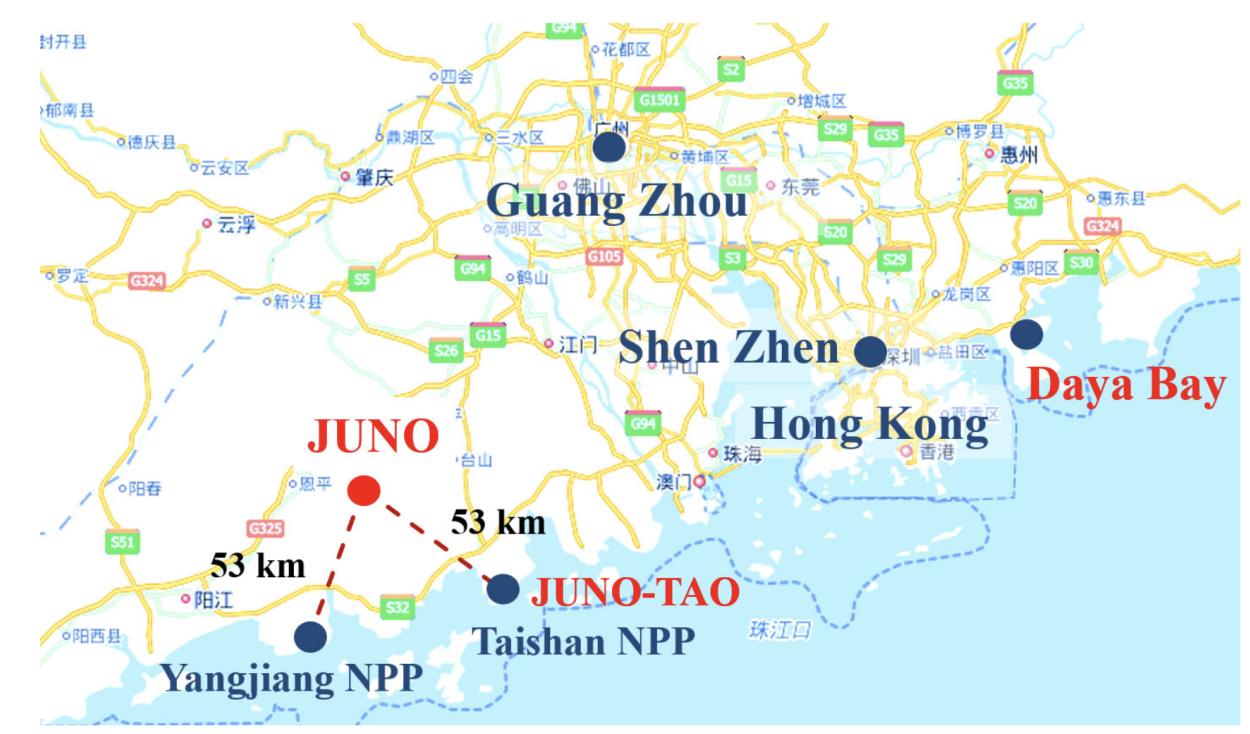
\includegraphics[width=\textwidth]{images/juno/juno_location.png}
  \end{subfigure}
  \hfill
  \begin{subfigure}[b]{0.48\textwidth}
    \centering
    \includegraphics[width=\textwidth]{images/juno/juno_outside.jpg}
  \end{subfigure}
  \caption{\textbf{On the left:} Location of the JUNO experiment and its reactor sources in southern china. \textbf{On the right:} external view of the experimental site}
\end{figure}

For this JUNO will measure the electronic anti-neutrinos ($\bar{\nu}_e$) flux coming from the nuclear reactors of Taishan, Yangjiang, for a total power of 26.6 GW$_{th}$, and the Daya Bay power plant to a lesser extent. Details about the power plants and there expected flux of $\bar{\nu}_e$ can be found in the table \ref{tab:power_plants}.
The distance of 53 km has been specifically chosen to maximize the disappearance probability of the $\bar{\nu}_e$.

\section{Neutrinos physics in JUNO}

\subsection{$\bar{\nu}_e$ flux coming from nuclear power plants}

To get such high measurements precision, it is necessary to have a very good understanding of the source characteristics. For its main studies, JUNO will measure the energy of neutrinos coming from core of nuclear power plants of Taishan and Yangjiang, located at 53 km of the detector to maximise the disappearance probability of the $\bar{\nu}_e$.

\begin{table}[ht]
  \centering
  \begin{tabular}{l c c c c}
    \hline
    Reactor & Power (GW$_{th}$) & Baseline (km) & IBD Rate (day$^{-1}$) & Relative Flux (\%) \\
    \hline
    Taishan    & 9.2  & 52.71 & 15.1 & 32.1 \\
    $~$ Core 1 & 4.6  & 52.77 & 7.5  & 16.0 \\
    $~$ Core 2 & 4.6  & 52.64 & 7.6  & 16.1 \\
    Yangjiang  & 17.4 & 52.46 & 29.0 & 61.5 \\
    $~$ Core 1 & 2.9  & 52.74 & 4.8  & 10.1 \\
    $~$ Core 2 & 2.9  & 52.82 & 4.7  & 10.1 \\
    $~$ Core 3 & 2.9  & 52.41 & 4.8  & 10.3 \\
    $~$ Core 4 & 2.9  & 52.49 & 4.8  & 10.2 \\
    $~$ Core 5 & 2.9  & 52.11 & 4.9  & 10.4 \\
    $~$ Core 6 & 2.9  & 52.19 & 4.9  & 10.4 \\
    Daya Bay   & 17.4 & 215   & 3.0  & 6.4  \\
    \hline
  \end{tabular}
  \caption{Characteristics of the nuclear power plants observed by JUNO. The IBD rate are estimated from the baselines, the reactors full thermal power, selection efficiency and the current knowledge of the oscillation parameters}
  \label{tab:power_plants}
\end{table}

The $\bar{\nu}_e$ coming from reactors are emitted from $\beta$-decay of unstable fission fragments. The Taishan and Yangjiang reactors are pressurised water reactor (PWR), the same type as Daya Bay. In those type of reactor more the 99.7 \% and $\bar{\nu}_e$ are produced by the fissions of four fuel isotopes $^{235}$U, $^{238}$U, $^{239}$Pu and $^{241}$Pu. The neutrino flux per fission of each isotope is determined by the inversion of the measured $\beta$ spectra of fission product \cite{hahn_antineutrino_1989, mueller_improved_2011, von_feilitzsch_experimental_1982, schreckenbach_determination_1985, huber_determination_2011} or by calculation using the nuclear databases \cite{vogel_reactor_1981, dwyer_spectral_2015}. The neutrino flux coming from a reactor at a time $t$ can be predicted using
\begin{equation}
  \phi(E_\nu, t)_r = \frac{W_{th}(t)}{\sum_i f_i(t) e_i} \sum_i f_i(t) S_i(E_\nu)
\end{equation}
where $W_{th}(t)$ is the thermal power of the reactor, $f_i(t)$ is the fraction fission of the $i$th isotope, $e_i$ its thermal energy released in each fission and $S_i(e_\nu)$ the neutrino flux per fission for this isotope. Using this method, the flux uncertainty is expected to be of an order of 2-3 \% \cite{juno_collaboration_sub-percent_2022}.

In addition to those prediction, a satellite experiment named TAO\cite{steiger_tao_2022} will be setup the reactor core Taishan 1 to measure with an energy resolution of 2\% at 1 MeV the neutrino flux coming from the core to identify unknown fine structure and give more insight on the $\bar{\nu}_e$ flux coming from this reactor.

\subsection{Reactor neutrino oscillation for NMO and precise measurements}

Previous works \cite{zhan_determination_2008,  zhan_experimental_2009} shows that oscillation parameters and the NMO can be observed by looking at the $\bnue$ disappearance spectrum coming from medium baseline nuclear reactor. This disappearance probability can be expressed as \cite{an_neutrino_2016} :
\begin{equation*}
  P(\bnue \rightarrow \bnue) = 1 - \sin^2 2\theta_{12} c^4_{13} \sin^2 \frac{\Delta m^2_{21}L}{4E} - \sin^2 2\theta_{13} \bigg[ c_{12}^2 \sin^2 \frac{\Delta m_{31}^2 L}{4E} + s^2_{12} \sin^2 \frac{\Delta m_{32}^2 L}{4E} \bigg]
\end{equation*}
Where $s_{ij} = \sin \theta_{ij}$, $c_{ij} = \cos \theta_{ij}$, $E$ is the $\bnue$ energy and $L$ is the baseline.
We can see the sensitivity to the NMO in the dependency to $\Delta m_{32}^2$ and $\Delta m^2_{31}$ causing a phase shift of the spectrum as we can see in the figure \ref{fig:juno-spectrum-oscillation}.
By carefully fitting this spectrum, one can extract the NMO and the oscillation parameters. The fit is reviewed in more details in the section \ref{sec:Fit}

\begin{figure}
  \centering
  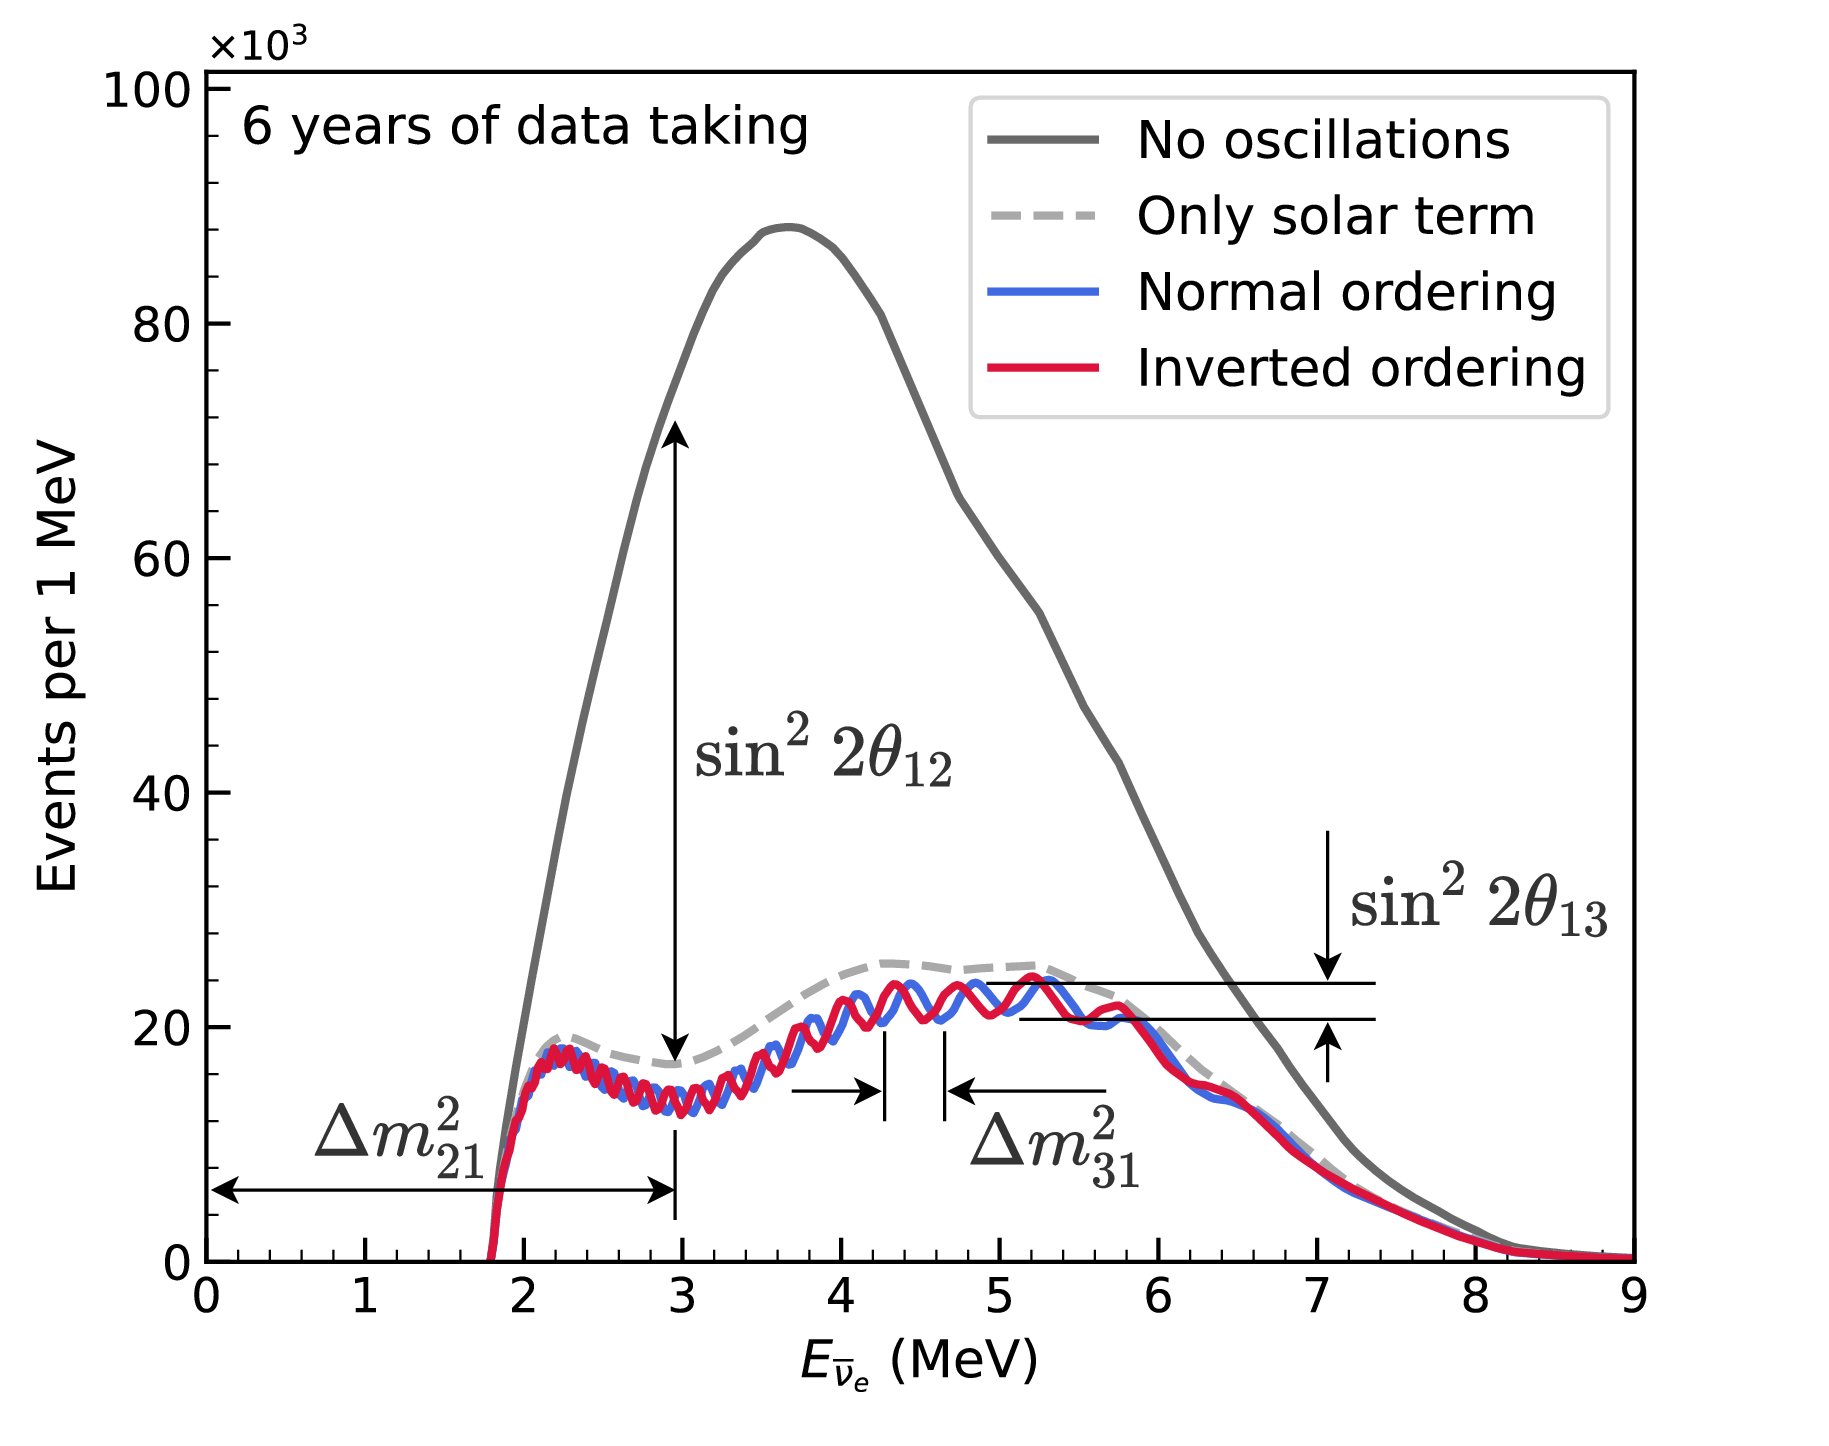
\includegraphics[height=8cm]{images/juno/Spectrum-OscillationsOnly_dm2_31.png}
  \caption{Expected number of neutrinos event per MeV in JUNO after 6 years of data taking. The black curve shows the flux if there was no oscillation. The light gray curve shows the oscillation if only the solar terms are taken in account ($\theta_{12}$, $\Delta m_{21}^2$). The blue and red curve shows the spectrum in the case of, respectively, NO and IO. The dependency of the oscillation to the different parameters are schematized by the double sided arrows. We can see the NMO sensitivity by looking at the fine phase shift between the red and the blue curve.}
  \label{fig:juno-spectrum-oscillation}
\end{figure}

To reach the desired sensitivity, JUNO must meet multiple requirements but most notably:
\begin{enumerate}
  \item An energy resolution of $3\%/\sqrt{E\mathrm{(MeV)}}$ to be able to distinguish the fine structure of the fast oscillation.
  \item An energy precision of 1\% in order to not err on the location of the oscillation pattern.
  \item A baseline of 53 $\pm$ 0.5 km to maximise the $\bar{\nu}_e$ oscillation probability.
  \item At least $\approx$ 100,000 events to limit the spectrum distortion dur to statistical uncertainties.
\end{enumerate}

\subsubsection{Identification of the mass ordering}

To identify the mass ordering, we fit the neutrino energy spectrum under the two hypothesis of NO and IO. Those two fit give us two $\chi^2$, respectively $\chi^2_{NO}$ and $\chi^2_{IO}$. By computing the difference $\Delta \chi ^2 = \chi^2_{NO} - \chi^2_{IO}$ we can determine the most probable mass ordering: NO if $\Delta \chi^2 > 0$ and IO if $\Delta \chi^2 < 0$. Current studies shows that the expected sensitivity the mass ordering would be of $3.4 \sigma$ after 6 years of data taking in nominal setup\cite{an_neutrino_2016}. More detailed explanations about the fitting procedure can be found in the section \ref{sec:Fit}.

\subsubsection{Precise measurement of the oscillations parameters}

The oscillations parameters $\theta_{12}$, $\theta_{13}$, $\Delta m^2_{21}$, $\Delta m^2_{31}$ are free parameters in the fit of the oscillation spectrum. The precision on those parameters have been estimated and are shown in figure \ref{fig:juno-param-precision}. Wee see that for $\theta_{12}$, $\Delta m^2_{21}$, $\Delta m^2_{31}$, precision at 6 years is better than the reference precision by an order of magnitude \cite{juno_collaboration_sub-percent_2022}

\begin{figure}[hb]
  \centering
  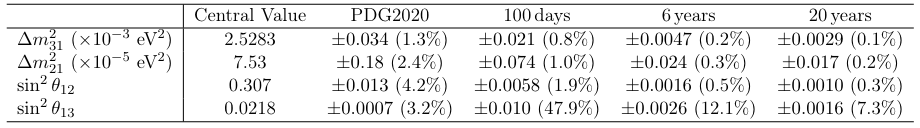
\includegraphics[width=\linewidth]{images/juno/oscillation_params_precision.png}
  \caption{A summary of precision levels fir the oscillation parameters. The reference value (PDG 2020 \cite{particle_data_group_review_2020}) is compared with 100 days, 6 years and 20 years of JUNO data taking.}
  \label{fig:juno-param-precision}
\end{figure}

\subsection{Other physics}

While the design of JUNO is tailored to measure $\bar{\nu}_e$ coming from nuclear reactor, JUNO will be able to detect neutrinos coming from other sources thus allowing for a wide range of physics studies as detailed in the table \ref{tab:signal} and in the following sub-section.

\begin{table}[ht]
\begin{center}
  \begin{tabular}{|c|c|c|c|}
    \hline Research & Expected signal & Energy region & Major backgrounds \\
    \hline Reactor antineutrino & 60 IBDs/day & 0–12 MeV  & Radioactivity, cosmic muon \\
    Supernova burst & 5000 IBDs at 10 kpc & 0–80 MeV & Negligible \\
                    & 2300 elastic scattering  & &  \\
    DSNB (w/o PSD) & 2–4 IBDs/year & 10–40 MeV & Atmospheric $\nu$ \\
    Solar neutrino & hundreds per year for $^8$B & 0–16 MeV & Radioactivity \\
    Atmospheric neutrino & hundreds per year & 0.1–100 GeV  & Negligible \\
    Geoneutrino &  $\approx 400$ per year & 0–3 MeV & Reactor $\nu$ \\
    \hline
  \end{tabular}
  \caption{Detectable neutrino signal in JUNO and the expected signal rates and major background sources}
  \label{tab:signal}
\end{center}
\end{table}


\subsubsection{Geoneutrinos}

Geoneutrinos designate the antineutrinos coming from the decay of long-lived radioactive elements inside the Earth. The 1.8 MeV threshold necessary for the IBD makes it possible to measure geoneutrinos from $^238$U and $^232$Th decay chains. The studies of geoneutrinos can help refine the Earth crust models but is also necessary to characterise their signal, as they are a background to the mass ordering and oscillations parameters studies.

\subsubsection{Atmospheric neutrinos}

Atmospheric neutrinos are neutrinos originating from the decay of $\pi$ and $K$ particles that are produced in extensive air showers initiated by the interactions of cosmic rays with the Earth atmosphere. Earth is mostly transparent to neutrinos below the PeV energy, thus JUNO will be able to see neutrinos coming from all directions. Their baseline range is large (15km $\sim$ 13000km), they can have energy between 0.1 GeV and 10 TeV and will contain all neutrino and antineutrinos flavour. Their studies is complementary to the reactor antineutrinos and can bring constraint on the MO \cite{an_neutrino_2016}.

\subsubsection{Beyond standard model neutrinos interactions}

JUNO will also be able to probe for beyond standard model neutrinos interactions. After that the main physics topics have been accomplished, JUNO could be upgraded to probe for neutrinoless beta decay ($0\nu\beta\beta$). The detection of such event would give critical informations about the nature of neutrinos, is it a majorana or a dirac particle. JUNO will also be able to probe for neutrinos that would come for the decay or annihilation of Dark Matter inside the sun and neutrinos from putative primordial black hole.
Through the unitary test of the mixing matrix, JUNO will be able to search for light sterile neutrinos.
Thanks to JUNO sensitivity, multiple other exotic can be performed on neutrino related beyond standard model interactions.

\subsubsection{Supernovae burst neutrinos}

Neutrinos are crucial component during all stages of stellar collapse and explosion. Detection of neutrinos coming for core collapse supernovae will provide us important informations on the mechanisms at play in those events.
Thanks to its 20 kt LS, JUNO has excellent capabilities to detect all flavour of the $\mathcal{O}$(10 MeV) postshock neutrinos, and using neutrinos of the $\mathcal{O}$(1 MeV) will give informations about the pre-supernovae neutrinos. All those informations will allow to disentangle between the multiple hydro-dynamic models that are currently used to describe the different stage of the core-collapse.

\subsubsection{Diffuse supernovae neutrinos background}

Core-collapse supernovae in our galaxy are rare events, but they frequently occur throughout the visible Universe sending burst of neutrinos in direction of the Earth. All those events contributes to a low background flux of low-energy neutrinos called the Diffuse Supernovae Neutrino Background (DSNB). Its flux and spectrum contains informations about the red-shift dependent supernovae rate, the average SN neutrino energy and the fraction of black-hole formation in core-collapse supernovae. Depending of the DSNB model, we can expect 2-4 IBD events per year in the energy range above the reactor $\bar{\nu}_e$ signal, which is competitive with the current Super-Kamiokande+Gadolinium phase.

\subsubsection{Background in the neutrinos reactor spectrum}

Considering the close reactor neutrinos flux as the main signal, the signals that are considered as background are:
\begin{itemize}
  \item The geoneutrinos producing background in the 0.511 $\sim$ 2.7 MeV region.
  \item The neutrinos coming from the other nuclear reactors around Earth.
\end{itemize}
In addition to all those physics signal, non-neutrinos signal that would mimic an IBD will also be present. It is composed of:
\begin{itemize}
  \item The signal coming from radioactive decay ($\alpha, ~ \gamma, ~ \beta$) from natural radioactive isotopes in the material of the detector.
  \item Cosmogenic event such as fast neutrons and activated isotopes induced by muons passing through the detector, most notably the spallation on $^12$C.
\end{itemize}
All those events represent a non-negligeable part of the spectrum as shown in figure \ref{fig:spectrum_with_background}.

\begin{figure}[ht]
  \centering
  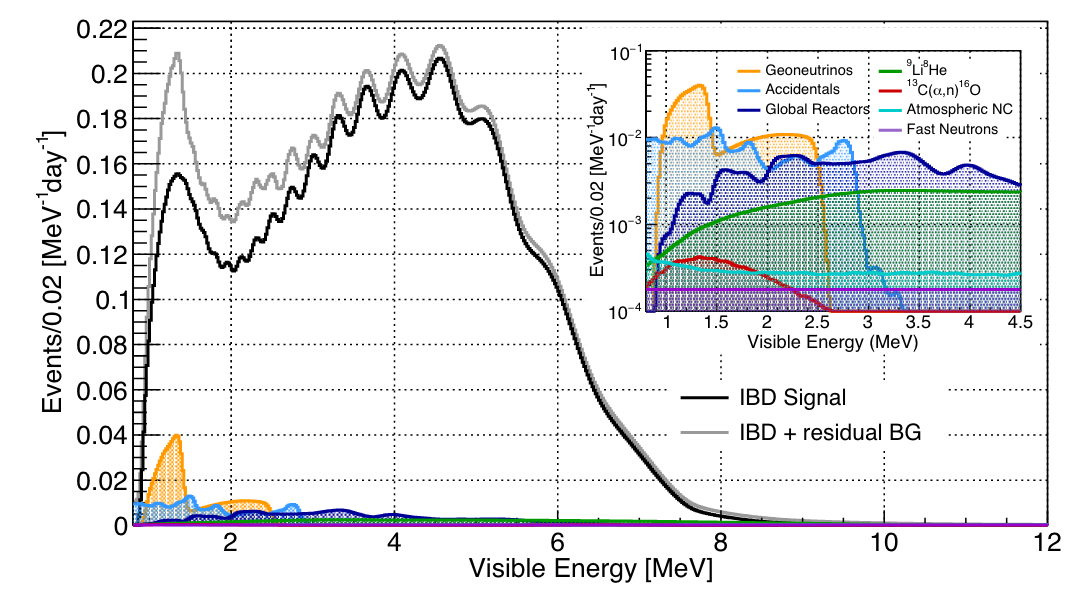
\includegraphics[height=6cm]{images/juno/spectrum_with_background.png}
  \caption{Expected visible energy spectrum measured with the LPMT system with (grey) and without (black) backgrounds. The background amount for about 7\% of the IBD candidate and are mostly localized below 3 MeV \cite{juno_collaboration_sub-percent_2022}}
  \label{fig:spectrum_with_background}
\end{figure}


\section{The JUNO detector}

\todo{1. Expliquer "grossierement" le detecteur, 2. Mettre ici toutes informations qui ne rentrerait pas dans les section suivantes (aka overburden, etc...)}

\subsection{Principle of detection}

JUNO will be able to detect neutrinos and measure their energy mainly via the Inverse Beta Decay (IBD) interaction
\begin{equation*}
  \bar{\nu}_e + p \rightarrow n + e^+
\end{equation*}
Simple kinematics calculation shows that the $\bar{\nu}_e$ must have an energy of $ (m_n + m_e - m_p ) \approx 1.806 ~ \mathrm{MeV}$ \cite{strumia_precise_2003} where $m_\lambda$ is the mass of the $\lambda$ particle.
This threshold make the experiment blind to very low energy neutrinos. The residual energy $E_{\nu} - 1.806 ~ \mathrm{MeV}$ is be distributed as kinetic energy between the positron and the neutron.
The energy of the emitted positron $E_e$ is given by \cite{strumia_precise_2003}
\begin{equation}
  E_e = \frac{(E_\nu - \delta)(1+\epsilon_\nu) + \epsilon_\nu \cos \theta \sqrt{(E_\nu - \delta)^2 + \kappa m_e^2}}{\kappa}
\end{equation}
where $\kappa = (1 + \epsilon_\nu)^2 - \epsilon_\nu^2 \cos^2 \theta \approx 1$, $\epsilon_\nu = \frac{E_\nu}{m_p} \ll 1$ and $\delta = \frac{m_n^2 - m_p^2 - m_e^2}{2m_p} \ll 1$.
We can see from this equation that the positron energy is strongly correlated to the neutrino energy.

Once the positron and the neutron will propagate in the detection medium, the liquid scintillator (LS), loosing their kinetic energy by exciting with the LS. Once stopped, the positron will annihilate with an electron from the medium producing two 511 KeV gamma. Those gamma will themselves interact with the LS, exciting it before being absorbed by photoelectrical effect. The neutron will be captured by an hydrogen, emitting a 2.2 MeV gamma in the process. This gamma will also deposit its energy before being absorbed by the LS.

\begin{figure}[ht]
  \centering
  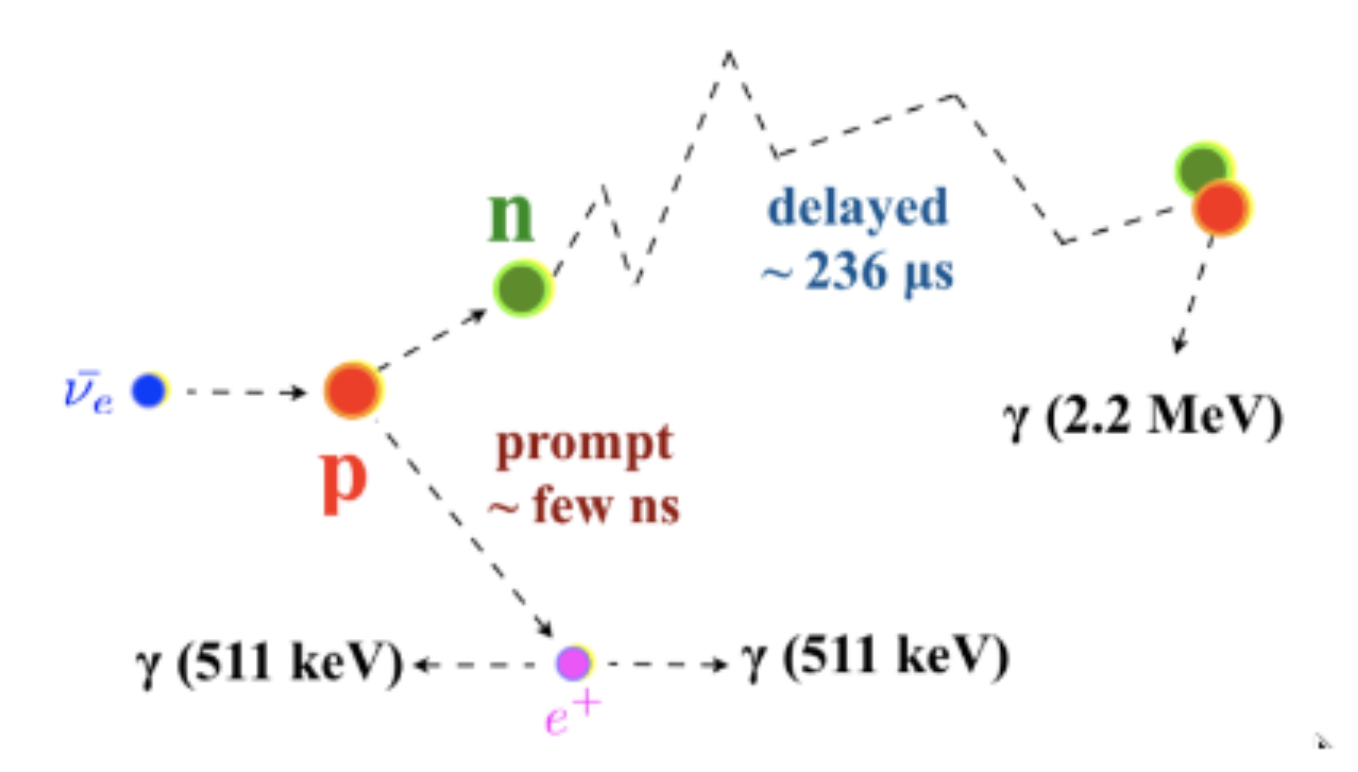
\includegraphics[width=8cm]{images/juno/IDB-JUNO.png}
  \caption{Schematics of an IBD interaction in the central detector of JUNO}
  \label{fig:IBD}
\end{figure}

More details about the LS can be found in section \ref{sec:CD}.

The scintillation photons will then be captured by the photo-multipliers (PMTs) surrounding the experiment. The analogue signal, then digitized by the electronic is the signal of our experiment. The signal produced by the positron is subsequently called the prompt signal, and the signal coming from the neutron the delayed signal. This naming convention come from the fact that the positron will deposit its energy rather quickly (few ns) where the neutron will take a bit more time ($\sim$ 236 $\mu$s).

\subsection{Central Detector (CD)}
\label{sec:CD}

\subsubsection{Acrylic containment sphere}

\subsubsection{Liquid scintillator}

\subsubsection{Large photo-multipliers (LPMTs)}

\subsubsection{Small photo-multipliers (SPMTs)}

\subsubsection{Data Acquisition System (DAQ)}

\subsubsection{Simulation}

\subsubsection{Software}

\todo{Expliquer comment le software fonctionne}


\subsection{Veto detector}

\subsubsection{Cherenkov in water pool}

\subsubsection{Top tracker}

\section{Calibration strategy}

\subsection{Energy scale calibration}

\subsection{Calibration system}

\subsection{Calibration program}

\section{Event selection and background rejection}

\todo{Explication de comment reconnaitre un IDB (OEC)}

\subsection{Fiducial volume}

\subsection{Muon tagging}

\section{State of the art of the IBD reconstruction}

\subsection{Interaction vertex reconstruction}

\subsection{Energy reconstruction}

\subsection{Particle identification}

\subsection{Machine learning for reconstruction}

\subsubsection{Vertex reconstruction}

\subsubsection{Energy reconstruction}

\section{JUNO sensitivity to NMO and precise measurements}

\subsection{Fitting procedure}
\label{sec:Fit}


\subfile{chapters/machine_learning}

\subfile{chapters/jcnn}

\subfile{chapters/jgnn}

\documentclass[../main.tex]{subfiles}
\graphicspath{{\subfix{..}}}

\begin{document}
\chapter{Reliability of machine learning methods}
\label{sec:janne}

\epigraph{``Psychohistory was the quintessence of sociology; it was the science of human behavior reduced to mathematical equations. The individual human being is unpredictable, but the reactions of human mobs, Seldon found, could be treated statistically''}{Isaac Asimov, Second Foundation}

\minitoc
%
% \textit{In this chapter I discuss the reliability of reconstruction algorithms, especially ML, in JUNO.}
%
% \textit{It is crucial for JUNO not only to reconstruct very precisely the energy of antineutrinos, but also to understand the quality of this reconstruction, and the differences in this between real data and the models assumed by the fits employed to perform the oscillation analysis.}
%
% \textit{We believe the first step in reliability studies is the comparison of the numerous reconstruction algorithms available in JUNO. In this goal, I present the implementation of a BDT for energy reconstruction that was developed by another scientist team in JUNO common software. I compare its resolution and behavior to OMILREC and use the combination method to probe for potential missing information in either of the algorithm}
%
% \textit{We also explore  the usage of an Adversarial Neural Network to produce perturbation in the event measurement (in recorded charge and time of PMT) that would distort the resulting energy spectrum while being invisible to the calibration.}
% \textit{I first discuss the method of this procedure, the Architecture that implement the method, the problematics and the implementation we present in this thesis. I finally present the training and the result obtained}
% \textit{We conclude this chapter by explaining that this first ANN prototype does not manage to generate perturbations that affect IBD events more than control sample events.  However, this exploration taught us several things, among which : it is very difficult to design an ANN able to introduce perturbations at the individual PMT level; some physics-informed guidance will be necessary to obtain an operational tool in the future.}
%
% \rule{\textwidth}{0.4pt}
As explained in previous chapters, JUNO is a precision experiment where a very precise understanding of the reconstruction effects is crucial. JUNO is a high-precision experiment, and any discrepancies in the understanding of reconstruction effects can significantly impact the neutrino mass ordering (NMO) determination. Particular attention must be paid to potential biases arising from energy scale miscalibration, charge non-linearity, and differences between real and simulated detector responses, which could skew the oscillation results.

While the liquid scintillator technology is well known, this is the first time it is deployed to such scale, and for such precision. This novelty bring makes this task difficult: a lot of effects should ideally be understood better that in previous experiments.
We already know that a bad knowledge of the energy scale can have consequences as serious as excluding the wrong NMO. It must be known at the 1\% level to reach the desired sensitivity. The present chapter is motivated by a specific question: even very small differences between reconstruction effects in real data and in the models used in oscillation fits could alter this sensitivity or bias the results. Reconstruction algorithms developed in JUNO, in particular those based on ML, try to use the information present in the detector as exhaustively as possible. This might apply even more to future algorithms. There is here a risk that some used information is not similar is real data and in the detector's model, leading to the problem mentioned above. We worked on two ways to address this concern.

We think the simpler way to study this reliability issue is to compare algorithm with each other. Differences between various reconstructed spectra of the same sample provide an envelope to evaluate the scale of a potential problem. Comparisons on the event per event basis allows showing that 2 algorithms do not use the same information, and is a first step to characterize this difference.
We already showed a large variety of reconstruction algorithms, OMILREC for LPMT reconstruction in Section \ref{sec:juno:reco}, numerous machine learning algorithms in Section \ref{sec:juno:ml} and our own work in Chapters \ref{sec:jcnn} and \ref{sec:jgnn}. Those algorithms were compared to each other based on their performance as in \cite{qian_vertex_2021} but we are the first that looked into the correlation between the reconstruction. The combinations of algorithms shown in Section \ref{sec:jcnn:combination} show that some information elude the algorithms. To efficiently compare algorithms between each other, they need to be publicly available to the collaboration to studies their differences, event by event.
Nothing of that kind was possible in JUNO up to now. I imported in JUNO's official software some tools necessary to ML algorithms, and I implemented a first algorithm:  a for energy reconstruction, named BDTE which was developed by Gavrikov et al.\ \cite{gavrikov_energy_2022}, another JUNO's research team. We paved the way for this movement to continue, so that all ML algorithms be available to any JUNO analyst. The details of this implementation and its combination with OMILREC are presented in Section \ref{sec:janne:BDTE}.

The other way we have explored to study reliability is to challenge reconstruction algorithms with physically plausible perturbations in the PMT charge and time information. More specifically: these perturbations embody differences between the real detector and its model,  and we want to identify perturbation patterns which  would be too subtle to be detected via data/MC comparisons in calibration data or in control samples from physics data, but which would still be able to alter the oscillation analysis result.  We could try to design such perturbations ``by hand'', based on our knowledge of JUNO. However, with as much as 17600 LPMT, finding subtle perturbations that affecting undefined combinations of PMT would be an endless process.

We propose leveraging machine learning by developing an Adversarial Neural Network (ANN) to introduce perturbations reflecting discrepancies between the real detector and its model. However, one challenge with ANN-based approaches is ensuring that the generated perturbations remain physically plausible and are not overly sensitive to random noise or edge effects in the detector.

In Section \ref{sec:janne:method}, I describe the method behind the algorithm. In Section \ref{sec:janne:arch} I detail the architecture of our algorithm.
The training and the results of our method are presented in Section \ref{sec:janne:arch:training}. Finally, in Section \ref{sec:janne:conclusion}, I conclude and discuss the prospects and possible improvements to bring to this work.


\section{First implementation of ML methods in JUNO's software}
\label{sec:janne:BDTE}

To study the reliability of reconstruction algorithms it's necessary to be able to compare their reconstruction performance event by event. To ease the process, it is important that they are publicly available. JUNO's common software, discussed in Section \ref{sec:juno:software}, is based on the SNiPER framework \cite{lin_application_2017} which allows the packaging of the different steps of JUNO's analysis, from Monte Carlo (MC) data generation to event reconstruction, including the propagation and interactions of the particles in the LS, the emission and propagation of the scintillation light, the simulation of the PMTs' waveform reconstruction, electronic effects and the trigger system.

This framework is modular, with each module being a C++ class bound in Python. The execution of successive algorithms is orchestrated via Python scripts.


We could have implemented the algorithms presented in Chapters \ref{sec:jcnn} and \ref{sec:jgnn}, but since these are themselves not trivial, we chose to start with a simpler ML algorithm that presents similar energy reconstruction performances as OMILREC: a Boosted Decision Tree (BDT) for energy reconstruction developed by Gavrikov Arsenii et al.\ \cite{gavrikov_energy_2022}.
This BDT, named BDTE, is based on an aggregated features approach where instead of providing an ML algorithm with low level information, namely the full list of $(Q,t)$ in LPMTs, a set of higher-level variables is designed based on physicist's common knowledge and then fed to the BDT. The list of the aggregated features used by the BDT is presented in Table \ref{tab:janne:bdte:features}. These higher-order variables are extracted from the charge $Q$ and hit time $t$ distribution. It also depends on two straightforward interaction vertex estimators.


The first one is the charge barycenter
\begin{equation}
  \label{eq:janne:bdte:cc}
  \vec{r}_{cc} = \frac{\sum_i \vec{r}_{PMT,i} Q_i}{\sum_i Q_i}
\end{equation}
where $i$ index the fired PMT, $\vec{r}_{PMT, i}$ is the position vector of the $i$-th PMT and $Q_i$ is the charge it collected.

The second estimator is the hit time barycenter
\begin{equation}
  \label{eq:janne:bdt:cht}
  \vec{r}_{ht} = \frac{1}{\sum_i \frac{1}{t_i + c}} \sum_i \frac{\vec{r}_{PMT, i}}{t_i + c}
\end{equation}
where $t_i$ is the time of collection of the $i$-th PMT and $c = 50$ ns a constant to prevent divergence when $t_i$ is 0.

\begin{table}[ht]
  \centering
  \begin{tabular}{|l | l|}
    \hline
    Feature & Description \\
    \hline
    AccumCharge             & Sum of the charge collected by every LPMT \\
    $R_{ht}               $ & Radius reconstructed by the hit time barycenter  \\
    $z_{cc}               $ & $z$ component of the vertex reconstructed by the charge barycenter \\
    $\sigma \text{PE}     $ & Standard deviation of the distribution of collected PE per PMTs \\
    $N_{PMT}              $ & Number of fired PMTs \\
    $\text{ht}_{Kurtosis} $ & Kurtosis of the hit time distribution \\
    $\text{ht}_{25\%-20\%}$ & Difference between the 25\% and 20\% percentiles of the hit time distribution \\
    $R_{cc}               $ & Radius reconstructed by the center of charge barycenter \\
    $\text{ht}_{5\%-2\%}  $ & Difference between the 5\% and 2\% percentiles of the hit time distribution \\
    $\langle \text{PE} \rangle$ & Mean number of PE collected per PMTs \\
    ${\cal J}_{ht}        $ & Jacobian of the hit time distrbution \\
    $\phi_{cc}            $ & $\phi$ component in spherical coordinate of the charge barycenter \\
    $\text{ht}_{35\%-30\%}$ & Difference between the 25\% and 20\% percentiles of the hit time distribution \\
    $\text{ht}_{20\%-15\%}$ & Difference between the 20\% and 15\% percentiles of the hit time distribution \\
    $\text{PE}_{35\%}     $ & Value of the 35\% percentile of the charge distribution \\
    $\text{ht}_{30\%-25\%}$ & Difference between the 30\% and 25\% percentiles of the hit time distribution \\
    \hline
  \end{tabular}
  \caption{Summary of the aggregated features used by the BDT to reconstruct the IBD energy. The charge barycenter and hit time barycenter vertex estimators are detailed in Eq. \ref{eq:janne:bdte:cc} and \ref{eq:janne:bdt:cht} respectively.}
  \label{tab:janne:bdte:features}
\end{table}

The performance of this BDT, as published by Gavrikov Arsenii et al., is reported in Figure \ref{fig:janne:bdte:orignal_perf}. This BDT is developed in Python using the XGBoost \cite{chen_xgboost_2016} library and originally consisted of a collection of Python scripts for the training and the evaluation.

As stated before, JUNO software is composed of C++ modules orchestrated through Python scripts. The technical challenge was to extract the data from the internal representation of the event in JUNO software, the Event Data Model (EDM), into a comprehensible format for Python. This task, which was previously done via data pre-processing by Python scripts, had to be internalized within the software. The computation of the aggregated features was migrated from the Python scripts into C++ modules. The final step was to fetch the reconstruction results of the algorithm into the C++ framework to save the results in the EDM. Some Python libraries were missing, notably XGBoost. A request to the collaboration was issued for the packaging of these libraries with the common software. As a workaround, the documentation of the algorithm contains the procedure to locally install the missing libraries.

We validated the consistency of the aggregated features between the original Python implementation and the JUNO software by comparing 1,000 events with the help of Arsenii. For the majority of the features, the relative difference between his and ours was either 0 or of the order of $10^{-15}$, except features: $R_{cc}$, $R_{ht}$, and $z_{cc}$. For these three features, the relative difference is about $10^{-6}$, which, while small, is still surprisingly high for numerical computation. The distributions of the relative differences for these features are presented in Figure \ref{fig:janne:feat_diff}.

We investigated the source of these discrepancies. The difference in computation environments -- Python using Numpy \cite{harris_array_2020} and C++ using the standard library in our case -- is most likely the cause. Since the discrepancies arise from the computation of the barycenter in Eq. \ref{eq:janne:bdte:cc} and \ref{eq:janne:bdt:cht}, they may result from differences in compiler optimization during the weighted sum calculation. We consider that these differences are still small enough that the performance of the BDT is unaffected.


\begin{figure}[ht]
  \centering
  \begin{subfigure}[t]{0.32\linewidth}
    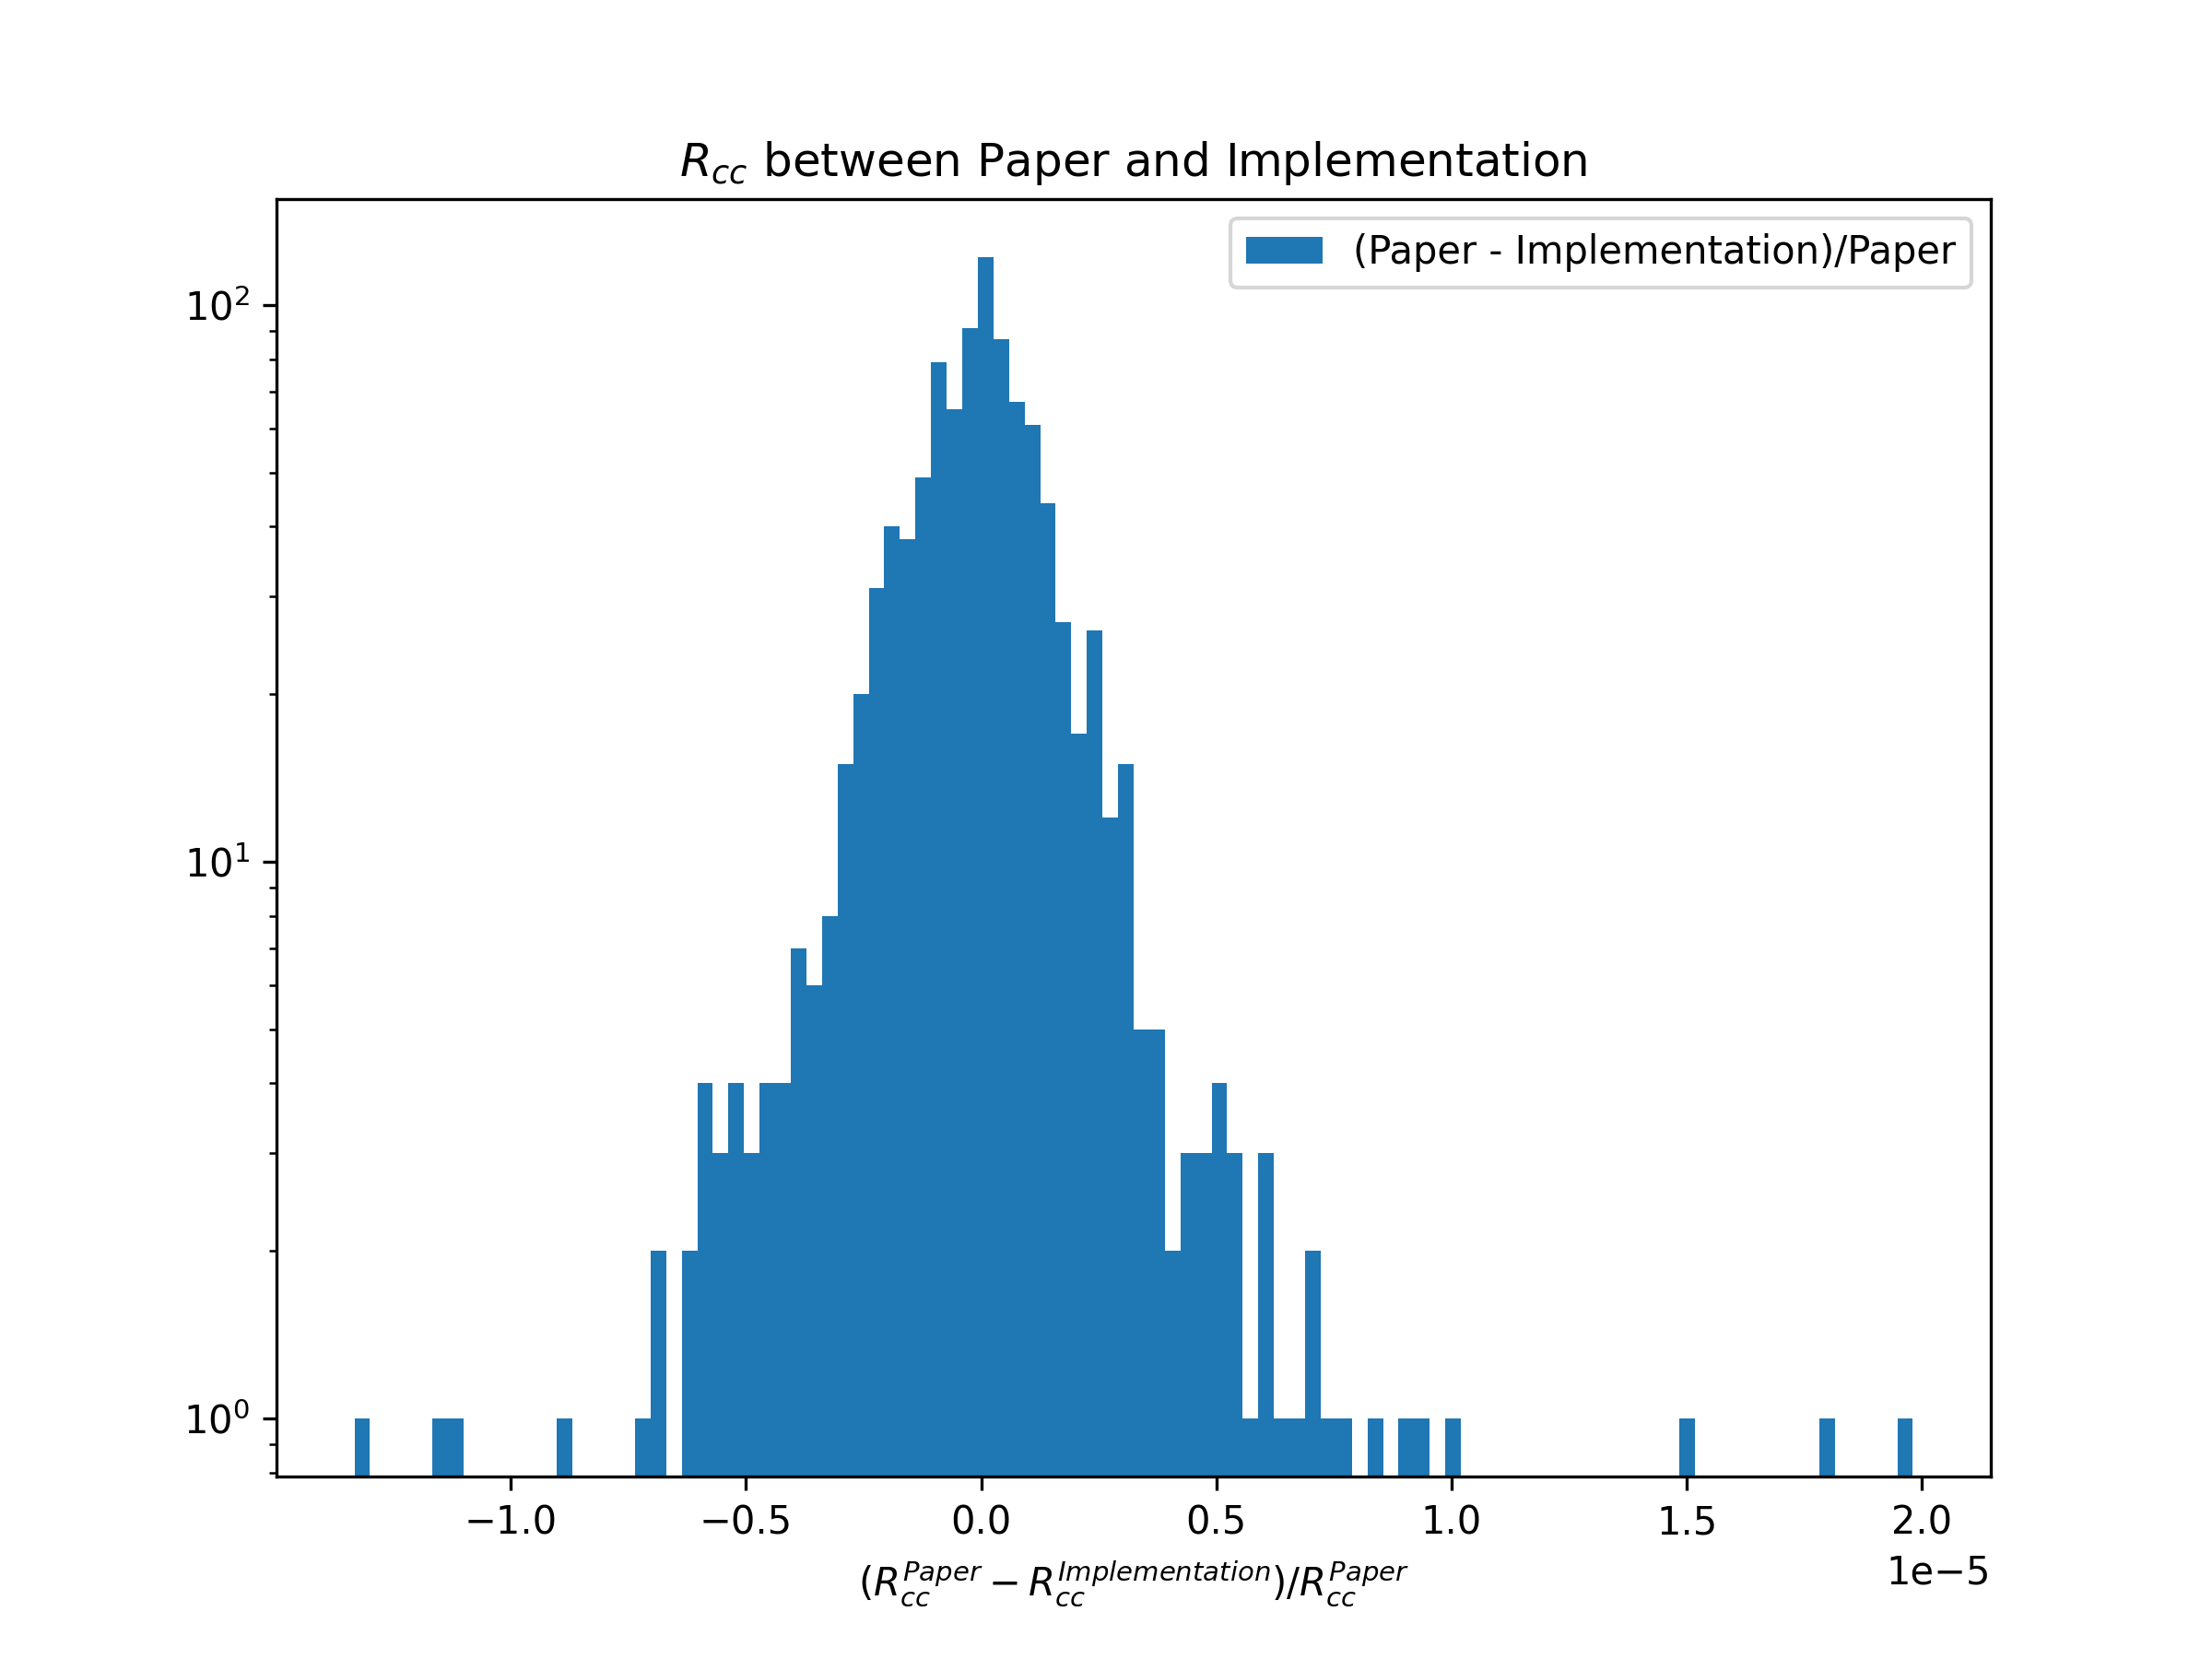
\includegraphics[width=\linewidth]{images/janne/bdte/R_cc_diff.png}
  \end{subfigure}
  \hfill
  \begin{subfigure}[t]{0.32\linewidth}
    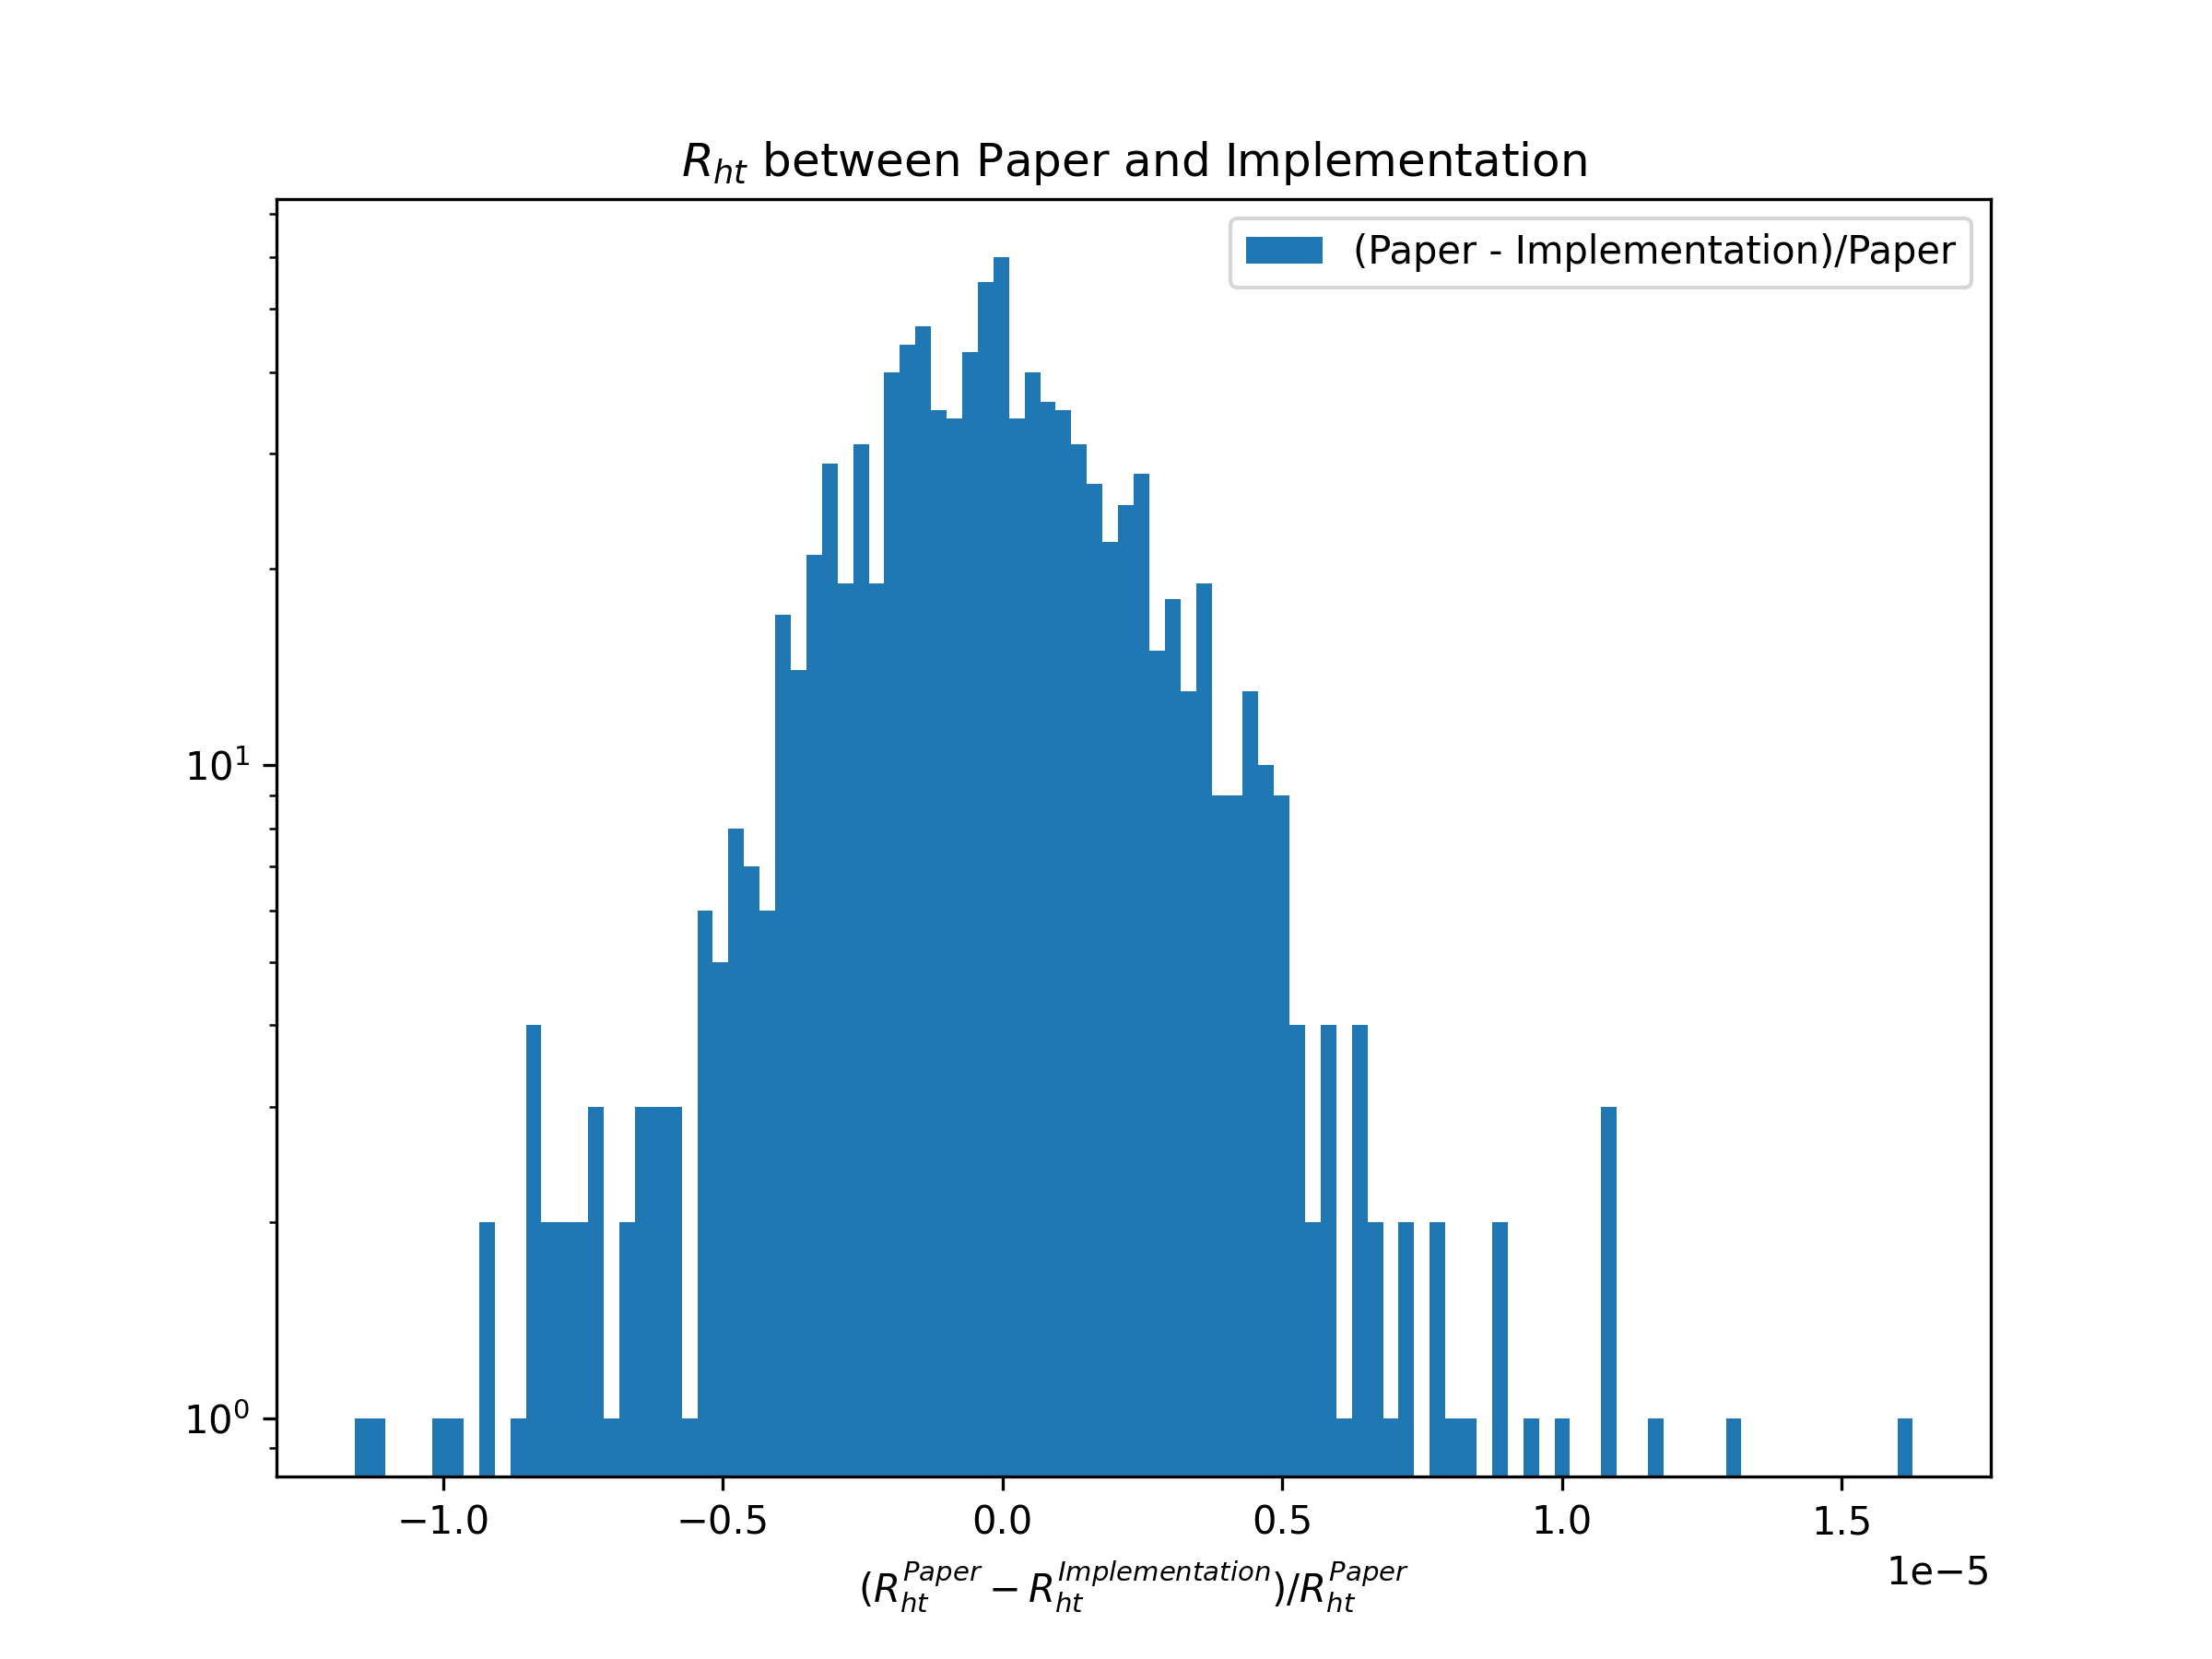
\includegraphics[width=\linewidth]{images/janne/bdte/R_cht_diff.png}
  \end{subfigure}
  \hfill
  \begin{subfigure}[t]{0.32\linewidth}
    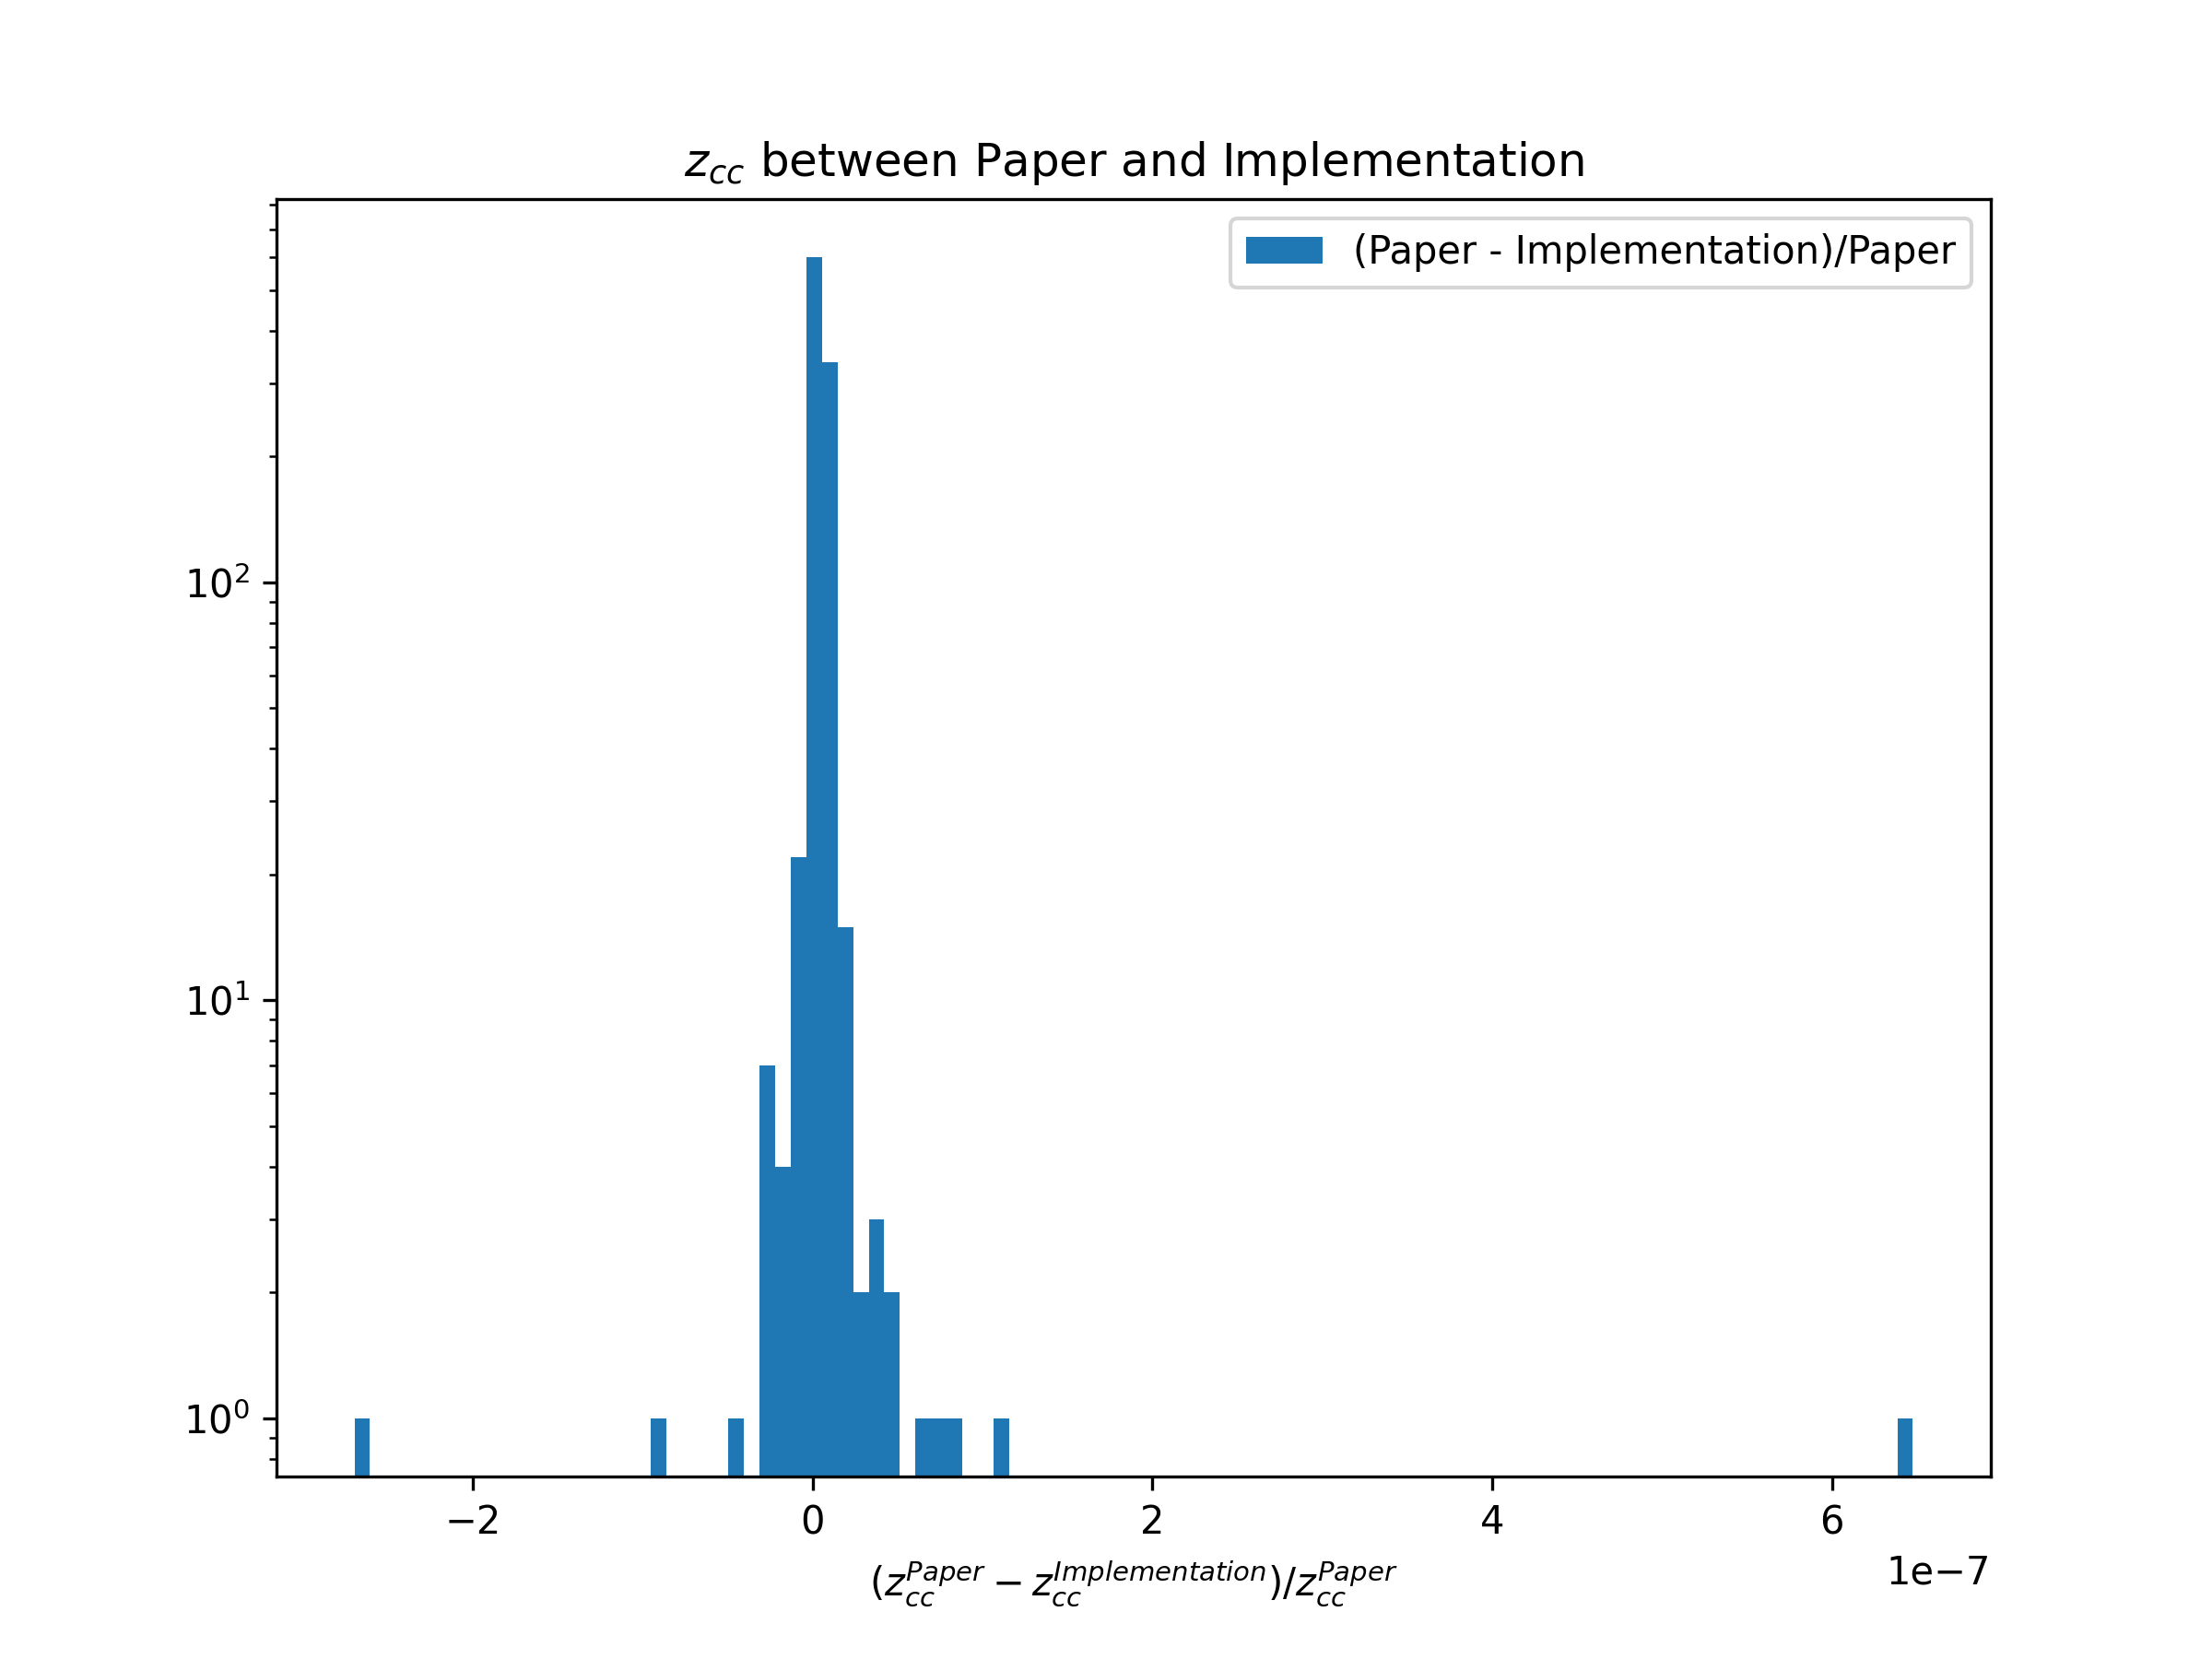
\includegraphics[width=\linewidth]{images/janne/bdte/z_cc_diff.png}
  \end{subfigure}
  \caption{Relative difference between the features computed by Gavrikov et al.\ (superscripted Paper) and our implementation (superscripted Implementation).}
  \label{fig:janne:feat_diff}
\end{figure}

The performance of our implementation of BDTE compared to the results presented in \cite{gavrikov_energy_2022} are presented in Figure \ref{fig:janne:bdte:implementation_perf}.
\begin{itemize}
  \item At 1 MeV, the relative resolution is reported by the publication is just below 3\%/MeV. Our implementation show a relative resolution of 2.8\%. The relative bias is reported at -0.1\%, same as for our implementation.
  \item At 4 MeV, the reported relative resolution is 1.5\%, our implementation show 1.45\%. The relative bias is about 0.05\% in both results.
  \item At 10 MeV, our implementation reconstruct the energy with a resolution of 1\% whereas the publication report a resolution a bit greater than 1\%. They report a positive relative bias of 0.05\% while we see a negative 0.1\%. This difference might come from the fact that Arsenii provided us an updated version of the BDT since the publication of \cite{gavrikov_energy_2022}.
\end{itemize}
The performance are considered compatibles.

\begin{figure}[ht]
  \centering
  \begin{subfigure}[t]{0.58\linewidth}
    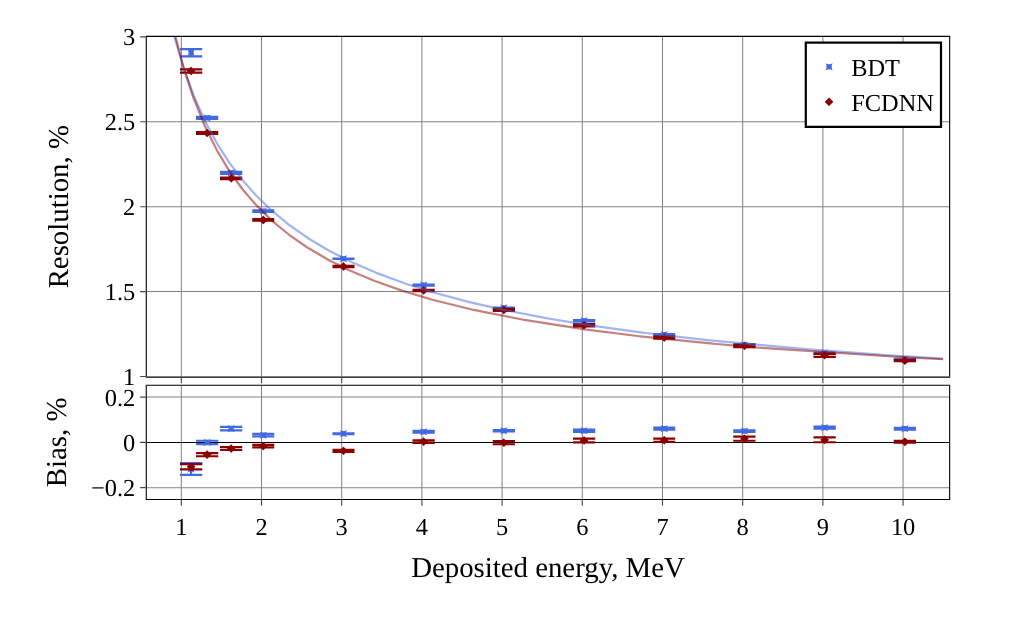
\includegraphics[width=\linewidth]{images/janne/bdte/bdte_perf.png}
    \caption{}
    \label{fig:janne:bdte:orignal_perf}
  \end{subfigure}
  \hfill
  \begin{subfigure}[t]{0.38\linewidth}
    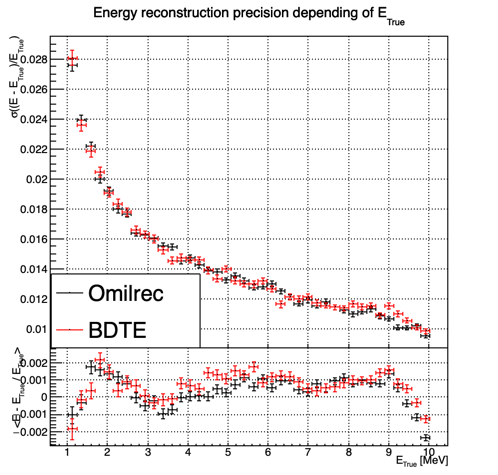
\includegraphics[width=\linewidth]{images/janne/bdte/e_rec_vs_e_true.png}
    \caption{}
    \label{fig:janne:bdte:implementation_perf}
  \end{subfigure}
  \caption{Resolution of BDTE \textbf{On the left: } as reported by Gavrikov Arsenii et. al in \cite{gavrikov_energy_2022}, \textbf{On the right: } once implemented in JUNO common software. On the right plot is also reported the reconstruction performance of the OMILREC algorithm. The OMILREC algorithm $E_{vis}$ has been corrected to $E_{dep}$ following the procedure detailed in Section \ref{sec:jgnn:results}.}
  \label{fig:janne:bdte:perf}
\end{figure}

The reconstruction using BDTE was implemented in JUNO's common software but Gavrikov et al.\ also detail the training and hyper-optimization. JUNO Monte Carlo is likely to evolve during the construction phase and will be further adjusted using calibration. The implementation of those procedures, the training and optimization, will be required as BDTE re-training and re-optimization will be required with each JUNO software update.

Figure \ref{fig:janne:bdte:implementation_perf} shows that the resolution of BDTE is very close to OMILREC. We measured the correlation between their reconstructions, focusing on the residuals with respect to the common true deposited energy:
\begin{equation}
  \label{eq:janne:bdte:corr}
\mathrm{Corr}(E_{BDTE} - E_{dep}, E_{OMILREC} - E_{dep})
\end{equation}

If the correlation is small enough, it indicates that these two reconstruction algorithms do not use the same information. As a corollary, it indicates that these algorithms can in principle be improved. The correlation between errors for different energy and event radius in the detector is presented in Figure \ref{fig:janne:bdte:corr}. We see that for the vast majority of the $(R^3, E)$ phase space, the correlation is > 0.995, down to $\sim$ 0.98 in the $R \approx 9$ m and $R > 17$ m regions. Such high correlations indicate that these algorithms are very close to using the same information. No difference can be found here, that could be used to improve them. Maybe the situation will be different when other ML algorithms are implemented in JUNO's software and the same exercise carried out. The fact that  BDTE and OMILREC are so correlated, and their performance so similar, is interesting: it suggests that using the full $(Q, t)$ list as inputs does not allow major improvements. This is in line with some conclusions we expressed in previous chapters: to improve  JUNO's reconstruction by starting from low level variables might require to use rawer variables than $(Q,t)$, like the full waveforms.

\begin{figure}
  \centering
  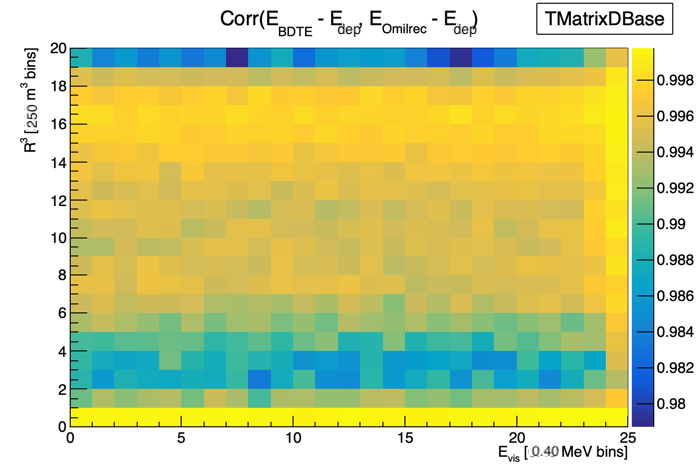
\includegraphics[height=7cm]{images/janne/bdte/corr_bdte_omilrec.png}
  \caption{Correlation between the errors in energy reconstruction between BDTE and OMILREC (Eq. \ref{eq:janne:bdte:corr}). The correlation is computed in $R^3$ bins of 216 m$^3$ between 0 and 5000 m$^3$, 0 and 17 m in y axis, and in 0.40 MeV bins between 1.022 and 10.022 MeV of deposited energy.}
  \label{fig:janne:bdte:corr}
\end{figure}



\section{Adversarial method}
\label{sec:janne:method}
%\begin{itemize}
%  \item JUNO needs very good understanding of reconstruction
%  \item Estimator combination shows that there can be improvement due to simplfication and that NN/reco methods can have hard time grasping all the detector effect.
%  \item If there is potential failure point, we need to search for them
%  \item La mesure de la NMO est tres sensible (see $alpha_{qnl}$ joint fit chapter)
%\end{itemize}

As introduced at the beginning of the chapter, JUNO needs a very good understanding of the biases and effects affecting its reconstruction, and small discrepancies between the real detector and its model could be an issue, in particular when ML algorithms are used. Calibration data will be used to study reconstruction effects and to tune the simulation so that the detector model matches as well as possible the real one. JUNO relies on multiple sources that can be deployed at various positions in the detector. The calibration strategy is already discussed in Section \ref{sec:juno:calib} and shows calibration sources of gammas, neutrons, and positrons (Table \ref{tab:juno:calib_source}), with the catch that the positrons will annihilate inside the encapsulation and only the two 511 keV gammas will deposit energy in the LS.

None of the calibration sources considered are positron events. While electrons and positron events should be pretty similar in their interaction with the electronic cloud of the LS atoms,
electron events are missing the two annihilation gammas. The topology of the event is therefore not the same: electron events display a single interaction site, up to a few cm longs, where a few MeV is deposited; positron events display a similar main site, accompanied by several others low energy (< 300 keV) sites, typically spread over more than 20 cm, due to the Compton interactions of the annihilation gammas. Other differences appear due to the fraction of the positrons that will  form a positronium: it causes a delay of a few nanoseconds between  energy deposition and the positronium annihilation, to be compared to the PMT  transit time spread between 3 and 6 ns, depending on the PMT type \cite{rodphai_20-inch_2021, liao_study_2017, li_characterization_2018}. Therefore, subtle effects might be present in positron events that the analysis of electron events samples cannot capture. Moreover, not all positions can be reached by calibration sources (effects affecting events close to the border of the detector can't be studied perfectly then), and calibration run are punctual in time, and therefore can't witness finely of time evolutions in the detector.

The two last issues presented above do not alter a natural source of calibration such as $^{12}B$ events. The $^{12}B$ is a cosmogenically produced isotope through the passage of muons inside the LS. The $^{12}B$ decays via $\beta^-$ emissions with a Q value of 13.5 MeV, with more than 98\% of the decay resulting in ground state $^{12}C$. This results into the e- energy spectrum shown on Fig. \ref{fig:juno:nl:boron}. The energy regime involved here is similar to that of reactor IBDs. The $^{12}B$ events will be cleanly identified by looking for delayed high-energy $\beta$ events after an energetic muon. The $^{12}B$ events will be uniformly distributed in the detector: moreover, $^{12}B$ events are produced continuously, and therefore can be used to follow finally time variations in the detector behavior. As with calibration sources, energy spectra obtained with measured and simulated $^{12}B$ events can be compared to control the accuracy of the detector model. This \textit{physics control sample} still presents the disadvantage to be an electron source.

The limitations of the calibration and control samples mentioned above could hide subtle data/MC discrepancies that might be able to bias the results of the oscillation analysis. We fear this problem in particular when ML algorithms are used, due to their ability to use exhaustively the information present in the detector.
But, while we have an idea of where the issues could come from, the manual production of event perturbations that go unseen when using these samples would be very time-consuming. That's why we propose to use the power of ML for an automated generation of adequate perturbation scenarios. We choose to develop an Adversarial Neural Network (ANN) to produce those perturbations if they exist. A schematic of the concept is presented in Figure \ref{fig:janne:method:schema}. We try here to extend to a large scale detector the concept introduced in \cite{nachman_ai_2019}.

\begin{figure}[ht]
  \centering
  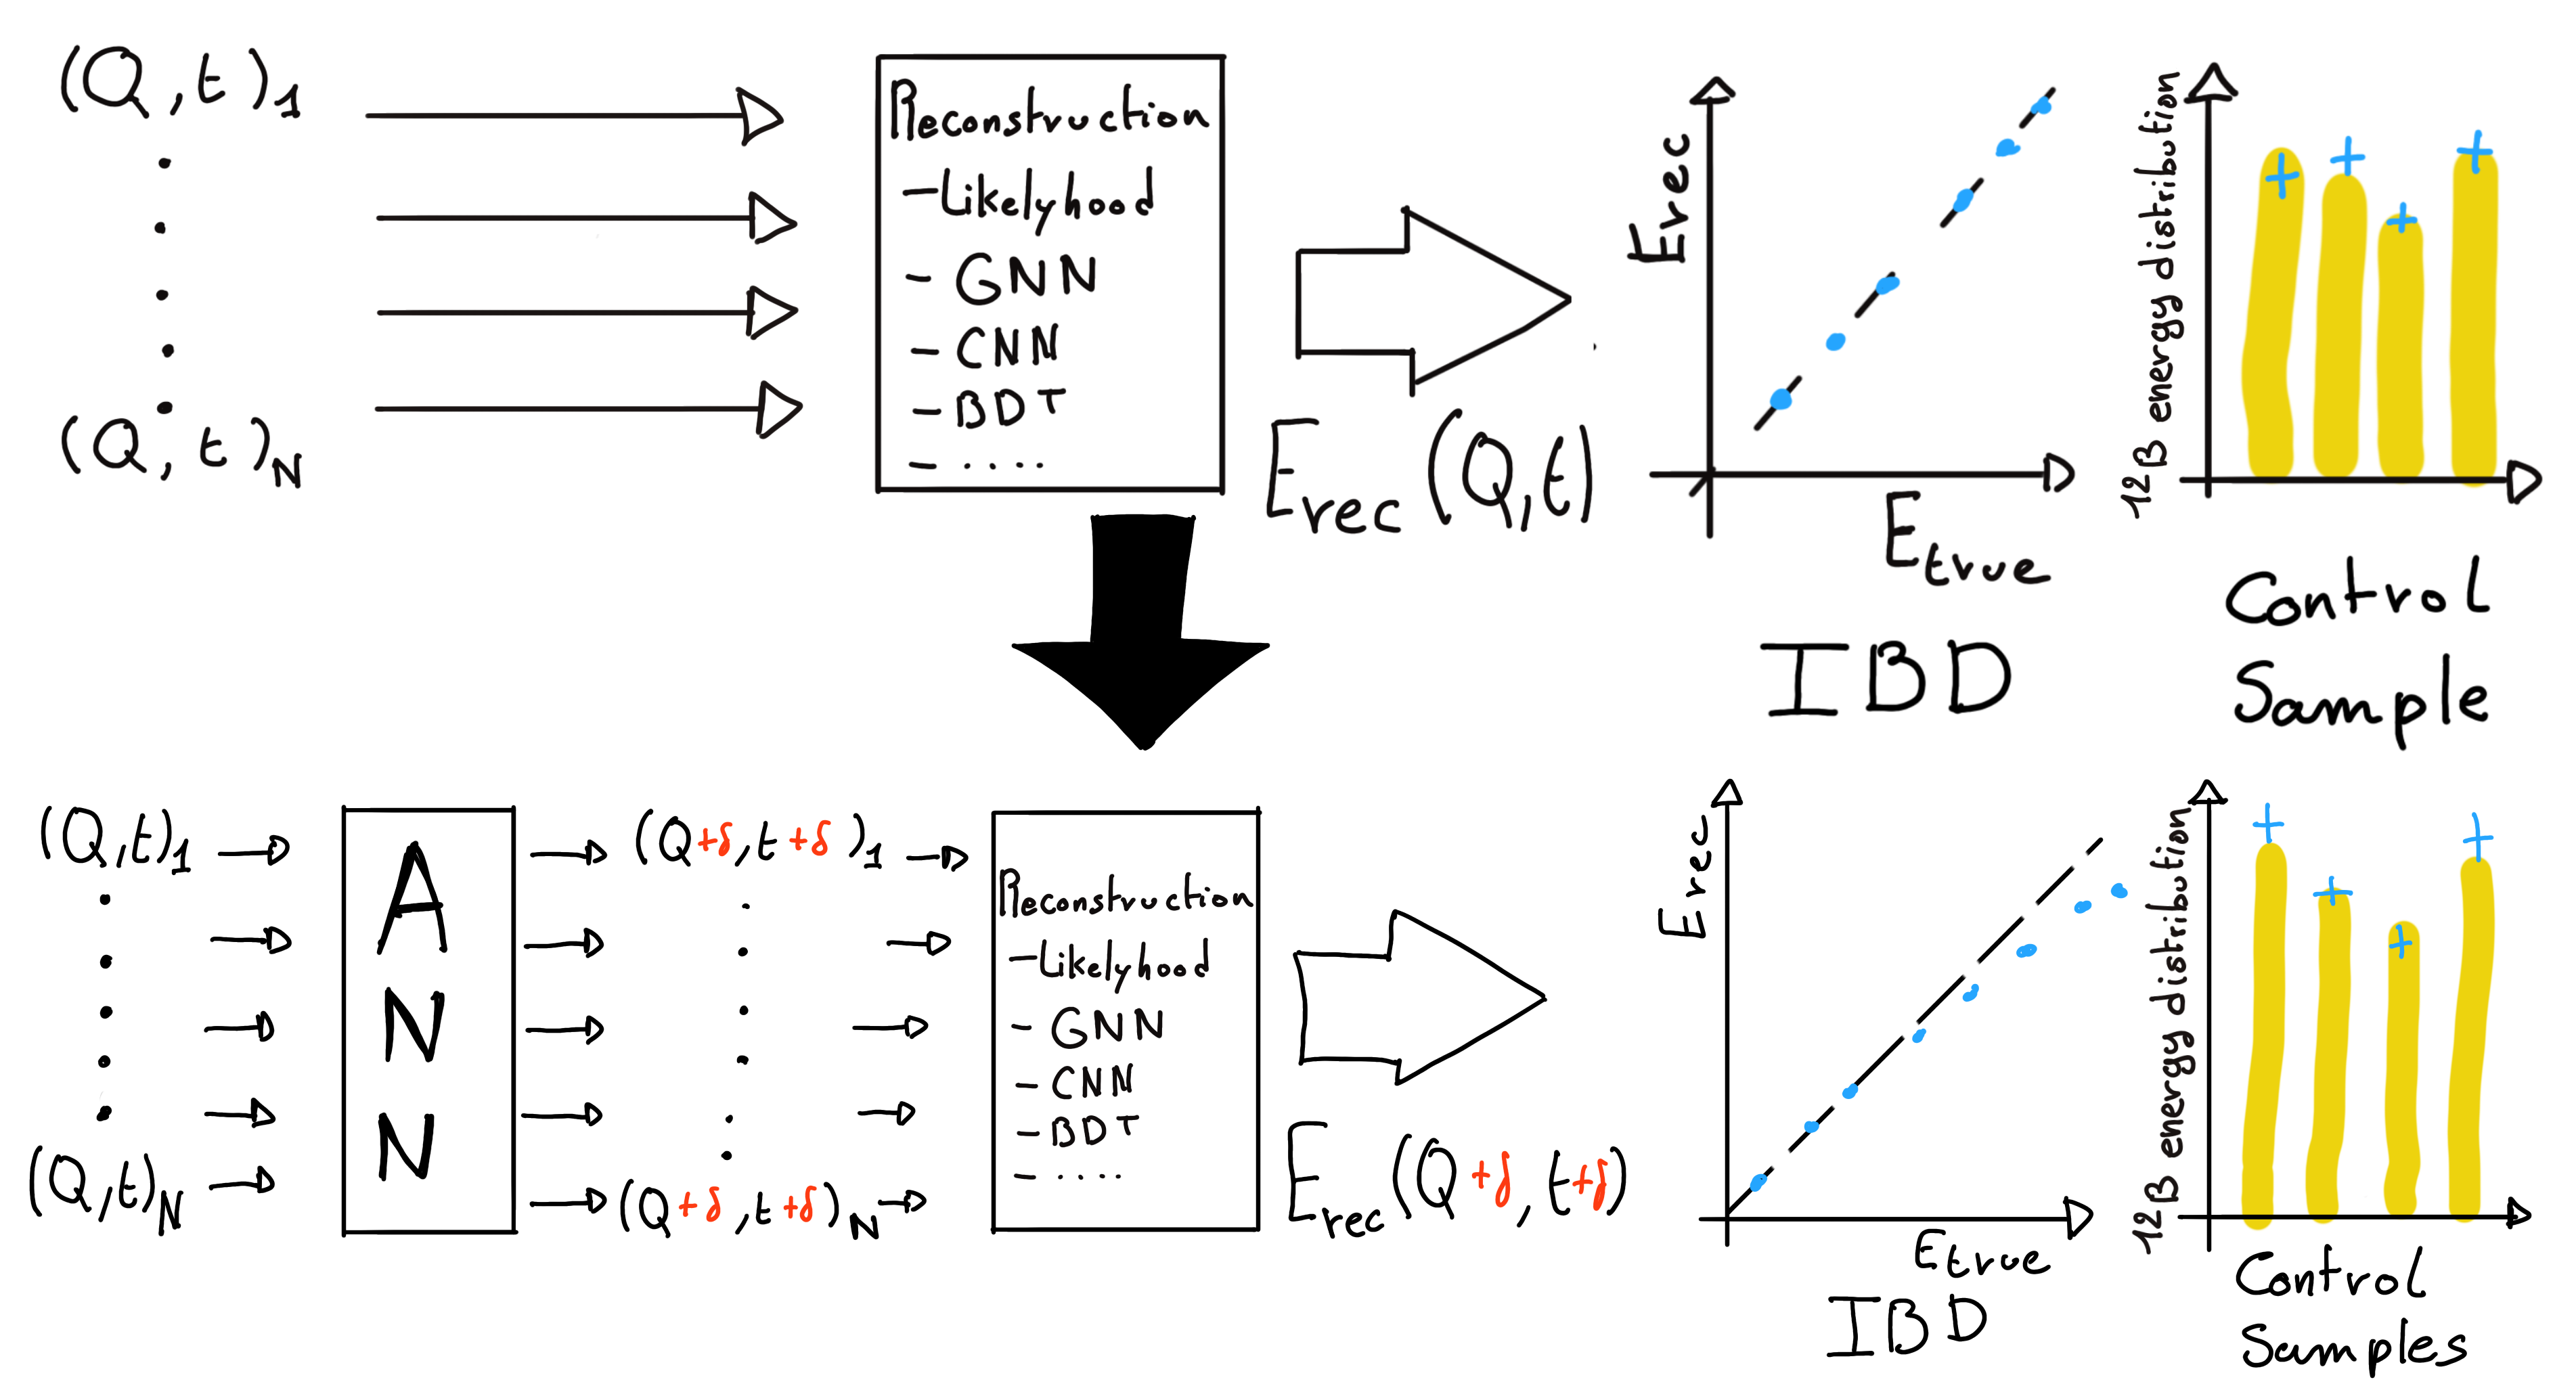
\includegraphics[width=\linewidth]{images/janne/ann_method.png}
  \caption{Schema of the method to discover vulnerabilities in the reconstruction methods. \textbf{On the top} of the image, the standard data flow. The individual charge and times are fed to a reconstruction algorithm. From the reconstructed energies, we can produce an IBD spectrum and compute control observables from the calibration and/or control samples (like a $^{12}B$ sample). In an ideal case, these observables should include the energy spectrum, the interaction position distributions, and any other useful variables. On the sketch above, the yellow distribution represent a real data sample while the blue points represents a simulated sample. \textbf{On the bottom}, the same data flow but we add an ANN between the input and the reconstruction. Still in an ideal case, the ANN learns what slight change to impose to each and every PMT so that the input charge and time so the reconstruction algorithm inaccurately reconstruct the IBD energy, but the perturbation is not visible in the control samples.}
  \label{fig:janne:method:schema}
\end{figure}

This network should produce physically plausible perturbations that would not be seen by the calibration system but also by the visualization of the event. If the ANN manages to produce such perturbations, we can derive systematic uncertainties from it. If it fails to find any, it is a proof of robustness for the targeted reconstruction method.

\subsection{ANN Architecture}
\label{sec:janne:arch}

For this study, we consider a ``physics'' dataset composed of 1M positron events from J23, uniformly distributed in the Central Detector (CD) and in deposited energy between $E_{dep} \in [1.022; 10.022]$. This set represents the IBD events we want to the reconstruction to be fooled on.

We use a second ``control'' dataset of 1M electron events from J23, also uniformly distributed in the detector and over the same energy range. They mimic the energy deposition of $^{12}B$ decay and are used as the sample to compute the control observables.

This work is a collaboration with an engineer from Subatech Gilles Grasseau. We, the JUNO's Subatech group, developed the idea and the global method design and the result interpretation. Gilles and I developed the ANN architecture, and Gilles the FFNN architecture. Gilles was in charge of the Python implementation and I provided the MC samples and readers to read the ROOT data into Python.



%\begin{itemize}
%  \item Expliquer la problematique dans l'architecture
%  \item Ambition de pouvoir etre appliqué a toutes les methodes, pas que NN
%  \item Pb techique: descente de gradient
%  \item Présenter la loss
%\end{itemize}
We can describe the goal of the ANN by using following loss function:
\begin{equation}
  \label{eq:janne:loss}
  \mathcal{L} = \mathcal{L}_{adv} + \mathcal{L}_{reg}
\end{equation}
where $\mathcal{L}_{adv}$ is the adversarial loss, which is minimal when the reconstruction is ``broken'', i.e.\ when the delta perturbations introduced on Fig \ref{fig:janne:method:schema} are at work. We thus need to define what is a \textit{wrong} reconstruction. We choose to define it through the correlation between the reconstructed and deposited energy
\begin{equation}
  \label{eq:janne:ladv}
  \mathcal{L}_{adv} = |\mathrm{Corr}(E_{rec}, E_{dep})|
\end{equation}
where $E_{rec}$ and $E_{dep}$ are the reconstructed energy and the true deposited energy respectively.
This loss is positive or null and is minimal when the reconstructed energy after perturbation is decorrelated with the true deposited energy. If this loss is below 1, there is a chance that the delta perturbations imposed on each PMT alter the result of the oscillation analysis. This loss is evaluated on the physics dataset.

The term $\mathcal{L}_{reg}$ is the regularization term, which is minimal when the control variables are correctly reconstructed
\begin{equation}
  \mathcal{L}_{reg} = \sum_\lambda (O^{rec}_\lambda - O^{th}_\lambda)^2
\end{equation}
where $\lambda$ index the different control observables that will be considered in this study. It's minimal when the control observables after perturbation $O^{rec}_\lambda$ are coherent with their expected values $O^{th}_\lambda$.
In this exploratory work, we pick as the control observable the difference between the reconstructed position and energy and the ground truth from the Monte Carlo simulation. When this loss is minimal, there is a chance that the perturbations will not be seen in data/MC  studies using this control sample, which is one of the goals of the algorithm.
\begin{equation}
  \label{eq:janne:lreg}
  \mathcal{L}_{reg} = \sum_{\lambda \in \{x, y, z, E\}} (\lambda_{rec} - \lambda_{true})^2
\end{equation}
This loss is evaluated on the control dataset.

To these two loss, we adjoin a penalty term $P$
\begin{equation}
  {\cal L} = {\cal L}_{adv} + {\cal L}_{reg} + P
\end{equation}
This penalty $P$ is here to prevent the ANN from producing event too different from the initial event. It will be further detailed in Section \ref{sec:janne:arch:ann}. This loss is evaluated on both datasets.

We see that the final loss is an equilibrium between the adversarial and regularization loss.

\subsection{Back-propagation problematic}
\label{sec:janne:back_prop}

We would like this method to be applicable to any kind of reconstruction algorithm, but this is complicated considering standard training method through backward-propagation (method discussed in details in Section \ref{sec:ml:optim}) for reasons developed in this section. This force use to develop, in this exploratory work, a new NN for reconstruction. This NN is presented in Section \ref{sec:janne:arch:reco}.

For explanation, let's define the application of the reconstruction algorithm as $\mathcal{F}$ on an event $X$, resulting in the prediction $Y$, and the application of the ANN $\mathcal{G}$ on $X$ to give a perturbed event $X'$. We can parametrize the equation \ref{eq:janne:loss}
\begin{align}
  Y = \mathcal{F}(X); ~~& Y' = \mathcal{F}(X') = \mathcal{F}(\mathcal{G}(X))
\end{align}
\begin{equation}
  \mathcal{L} \equiv \mathcal{L}(\mathcal{F}(\mathcal{G}(X)), Y_t)
\end{equation}
where $Y_t$ is the reconstruction target of $Y$.

Now if we consider the learnable parameters $\bm{\theta}$ of the ANN on which we want to optimize $\mathcal{L}$, in the backward-propagation optimization framework we need to compute
\begin{equation}
  \frac{\partial \mathcal{L}(\mathcal{F}(\mathcal{G}(X)))}{\partial \bm{\theta}}
\end{equation}
which, when using the chain rule, become
\begin{equation}
  \frac{\partial \mathcal{L}(\mathcal{F}(\mathcal{G}(X)))}{\partial \bm{\theta}} = \frac{\partial \mathcal{G}}{\partial \bm{\theta}} \cdot \frac{\partial \mathcal{F}}{\partial \mathcal{G}} \cdot \frac{\partial \mathcal{L}}{\partial \mathcal{F}}
\end{equation}

The terms $\frac{\partial \mathcal{G}}{\partial \bm{\theta}}$ and $\frac{\partial \mathcal{L}}{\partial \mathcal{F}}$ are easily computable but $\frac{\partial \mathcal{F}}{\partial \mathcal{G}}$ depends on the nature of the reconstruction algorithm.


While this term comes naturally when using neural network algorithms, its computation is embedded in most of modern framework, it's not so trivial for other types of algorithms like likelihood. Solutions exist to optimize networks that work in complex, non-differentiable environments, such as \textit{Deep Reinforcement Learning} \cite{kiran_deep_2021, vinyals_grandmaster_2019}, but as a first prototype, we will restrict ourselves to neural networks for the reconstruction algorithm.

The choice to use gradient descent, and therefore neural networks, also allowed us to keep all technical software development wrapped in the same language and framework, PyTorch \cite{ansel_pytorch_2024}.

The backward-propagation introduce a second issue. At the beginning of the subsection we introduce $X' = \mathcal{G}(X)$, the event after perturbation. It's an input of the reconstruction $\mathcal{F}$, thus, let's say that the event, in its form $X$, is a list of tuples $(id, Q, t)$ which are the hit on the PMT $id$. If $\mathcal{F}$ require the information to be formatted in a specific way (graph, images, $\ldots$) via an algorithm $\tau(X)$, it means that
\begin{equation}
  \frac{\partial \mathcal{L}(\mathcal{F}(\tau(\mathcal{G}(X))))}{\partial \bm{\theta}} = \frac{\partial \mathcal{G}}{\partial \bm{\theta}} \cdot \frac{\partial \tau}{\partial \mathcal{G}} \cdot \frac{\partial \mathcal{F}}{\partial \tau} \cdot \frac{\partial \mathcal{L}}{\partial \mathcal{F}}
\end{equation}
which also requires that $\frac{\partial \tau}{\partial \mathcal{G}}$ is differentiable.

On the other hand, if $X$ is already formatted as the input of ${\cal F}$, it means that ${\cal G}$ takes the same format as input, and we drop the requirement on $\tau$ to be differentiable. Specifically, if ${\cal F}$ takes an image as input, it means that ${\cal G}$ will also take an image as input and output an image. Unfortunately, this also means that if some information is lost before ${\cal G}$, for example, during the charge and time aggregation in pixels, the ANN cannot retrieve and modify it.

A more elegant solution would that $\mathcal{G}$ would also compute the transformation $\tau$ in addition to finding relevant perturbation, but for the simplicity of this exploratory work, we use a $\mathcal{G}$ that process transformed data.

\subsection{Reconstruction Network (FFNN)}
\label{sec:janne:arch:reco}
%\begin{itemize}
%  \item Reseau de Neurone Simple. Deux avantages:
%  \item Besoin pour la descente de gradient
%  \item Un reseau "simpliste" a plus de chance de présenter des "défauts" que l'ANN pourrait exploiter
%\end{itemize}

As introduced just before, we need a NN algorithm for IBD reconstruction. We could have used the GNN presented in Chapter \ref{sec:jgnn}, but we preferred a simpler approach to not be constrained by the memory consumption of the reconstruction network. The memory issue does not really come from the reconstruction network but from the ANN. The requirement to produce outputs that have the same structure and complexity as the reconstruction network makes it even more memory consuming than the reconstruction network, thus the choice for a simpler reconstruction network. This network is designated as FFNN for ``F''-Fully connected Neural Network where ``F'' is reminder to the ${\cal F}$ from previous section.

This network takes as input a vector containing the results of the aggregation of charge and time on pixels, forming a vectorized image. We consider JUNO to be composed of 3072 pixels defined by the HealPix \cite{gorski_healpix_2005} pixelization. On each of these pixels, we sum the charges and keep the first time of hit, resulting in 3072 $(Q,t)$ tuples. To these tuples, we adjoin the position of the center of these pixels, resulting in 3072 $(Q,t,x,y,z)$ tuples. The data is finally represented as a $3072 \times 5 = 15360$ vector. In the case where the charge in a pixel is 0, the time is set to 2048 ns, which is way after the closure of the trigger window.

The charge is expressed in $N_{pe}$ and the time of hit in nanoseconds. The time is negative, meaning that 0 ns the first hit time and -2048 ns is the latest hit time.

FFNN is a Fully Connected Neural Network (FCDNN) composed of the following layers: the input layer, providing the 15360-item vector, followed by fully connected linear layers with the respective number of neurons being $[8192,4096,2048,1024,512,256,128,64,32]$. These layers possess a Leaky ReLU activation function defined as

\begin{equation}
  \mathrm{LeakyReLU} = \begin{cases}
    x, & \text{if } x > 0 \\
    10^{-2} \cdot x, & \text{otherwise}
  \end{cases}
\end{equation}

The last layer is a linear layer with 4 neurons, representing $(x,y,z,E)$ without an activation function.


The loss used is the Mean Square Error (MSE)
\begin{equation}
  \text{MSE}(\bm{\eta}, \bm{\eta}^{true}) = \sum_i (\eta_i - \eta_i^{true})^2
\end{equation}
where $\eta$ takes the values of $(x, y, z, E)$.

The optimizer used for its training is the Stochastic Gradient Descent with momentum
\begin{equation}
  \bm{\theta}_{t+1} = \bm{\theta}_t - \Lambda \left(\sum_{i=0} \frac{\partial \mathcal{L}}{\partial \bm{\theta}_{t - i}} \cdot 0.9^{i} \right)
\end{equation}
where $\bm{\theta}_t$ is vector of learnable parameters at step $t$. $\Lambda$ is the learning rate set at  $10^{-3}$. The difference with the classical SGD is the gradient term with $i > 1$. We save the gradient computed in the previous step and use them as momentum with a decaying weight. The factor 0.9 is a hyperparameter that has been selected for the training.

Additionally, to prevent over-fitting, we introduce a weight decay. Each step, we reduce the amplitude of the parameters $\bm{\theta}$ by $10^{-3}$:
\begin{equation}
  \bm{\theta}_{t+1} = \bm{\theta}_t \cdot (1 - 10^{-3})
\end{equation}

\subsubsection{Performances}

The FFNN is trained independently of the ANN. The dataset is composed of 1M positrons events uniformly distributed in the detector and in energy over $E_{dep} \in [1, 10]$ MeV. The training dataset account for 990'000 events with 10'000 events reserved for validation. The data are normalized, mean shifted to 0 and standard deviation scaled to 1, before being processed by the network.

Each epoch go through the entire training datasets, with a batch size of 64. The training last for 25 epochs. The performance the FFNN are presented in Figures \ref{fig:janne:ffnn:ESB} and \ref{fig:janne:ffnn:SB}. We remind that goal of this FFNN is not to have competitive performances against classical algorithms like OMILREC but more to have a simple, NN reconstruction algorithm to run the ANN against.

\begin{figure}[ht]
  \centering
  \begin{subfigure}[t]{0.48\linewidth}
    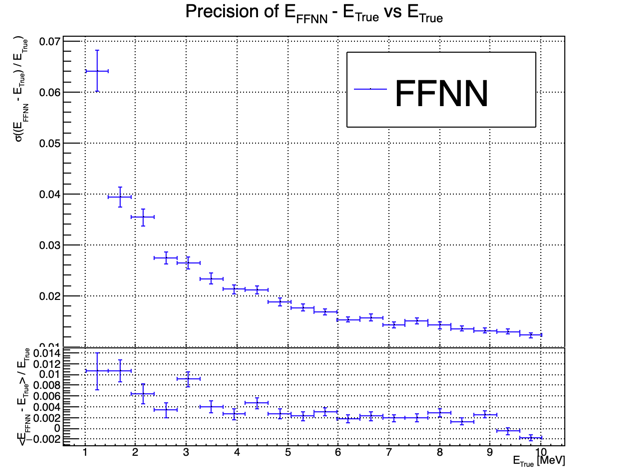
\includegraphics[width=\linewidth]{images/janne/ffnn/ESBE.png}
  \end{subfigure}
  \hfill
  \begin{subfigure}[t]{0.48\linewidth}
    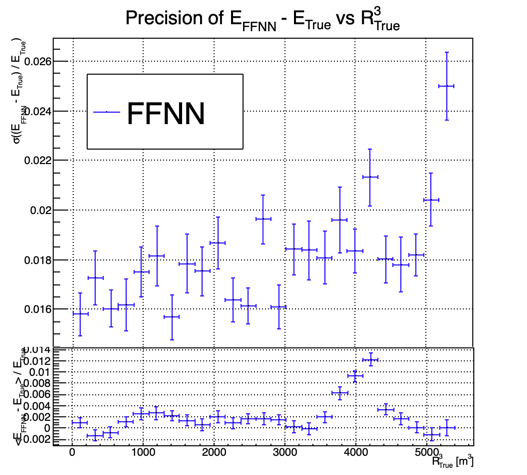
\includegraphics[width=\linewidth]{images/janne/ffnn/ESBR.png}
  \end{subfigure}
  \caption{Energy resolution of the FFNN with respect to the energy (\textbf{On the left}) and with respect to the radius (\textbf{On the right}).}
  \label{fig:janne:ffnn:ESB}
\end{figure}

\begin{figure}[ht]
  \centering
  \begin{subfigure}[t]{0.48\linewidth}
    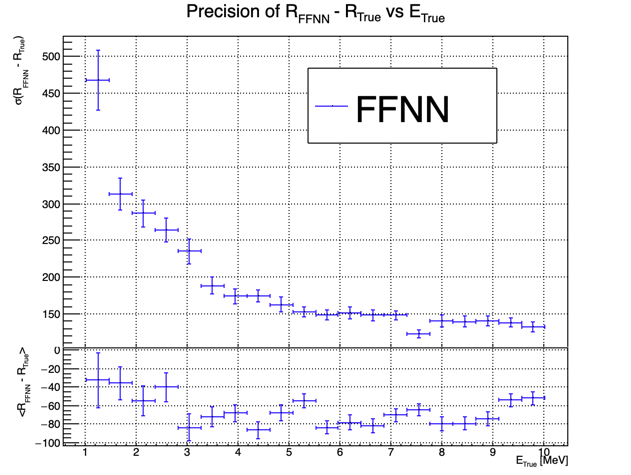
\includegraphics[width=\linewidth]{images/janne/ffnn/SBE.png}
  \end{subfigure}
  \hfill
  \begin{subfigure}[t]{0.48\linewidth}
    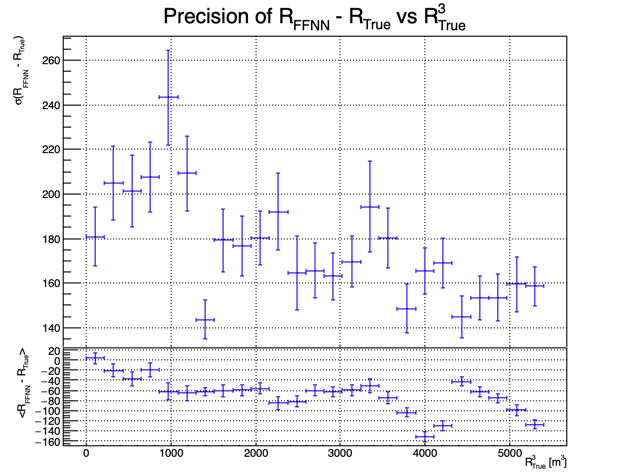
\includegraphics[width=\linewidth]{images/janne/ffnn/SBR.png}
  \end{subfigure}
  \caption{Radial resolution of the FFNN with respect to the energy (\textbf{On the left}) and with respect to the radius (\textbf{On the right}).}
  \label{fig:janne:ffnn:SB}
\end{figure}

\subsection{Adversarial Neural Network (ANN)}
\label{sec:janne:arch:ann}
%\begin{itemize}
%  \item Decrire l'architecture de l'ANN
%\end{itemize}

The ANN aims to introduce perturbations in the event data in such a way that these perturbations are not detectable in the control dataset while still degrading the energy reconstruction of the IBD dataset. For this purpose, and for the reasons detailed in Section \ref{sec:janne:back_prop}, the ANN operates on the inputs of the reconstruction network presented above, namely the FFNN. During the training, the parameters of the FFNN are \textit{frozen,} meaning they will not be updated during the ANN training. If they were free to be optimized, they would adapt to the perturbations of the ANN, which would go against the objective of this work.

The FFNN takes as input a vector of $5 \times 3072$ values, representing the $(x,y,z,Q,t)$ of 3072 HealPix pixels (pixelization illustrated in Figure \ref{fig:jgnn:healpix}). Those values come from the aggregation of the PMTs belonging to those pixels.

It seems unreasonable that the ANN would modify the HealPix pixel positions, as they are derived from a mathematical construction. It could, however, perturb which PMTs are assigned to specific pixels, introducing localization errors, but the position of the PMTs is carefully monitored during JUNO's construction. Such aggregation errors would likely arise from PMTs located at the edges of the pixels, yet this scenario seems unlikely. Moreover, due to the constraints mentioned in Section \ref{sec:janne:back_prop}, the ANN is required to work with the same format that the FFNN uses as input.


At the start of the project, we attempted to have it operate on both time and charge information simultaneously, but it struggled to converge. After discussions with colleagues in the collaboration, we decided that the ANN would only introduce perturbations in the charge information, as most of the energy information comes from the charge.

Our ANN thus needs to output a 3072-dimensional vector, which represents the updated charges of the detector.

We decided on a Fully Connected Deep NN (DNN) ``bottleneck'' architecture for the ANN, illustrated in Figure \ref{fig:janne:ann_arch}. This architecture places a 4096-neuron-wide layer after the input, followed by smaller layers of sizes 2048, 1024, and 512 neurons, before finally reaching the 256-neuron layer. From this layer, the size increases again to 512, 1024, and finally 2048 neurons before the output layer, which consists of 3072 neurons.


\begin{figure}
  \centering
  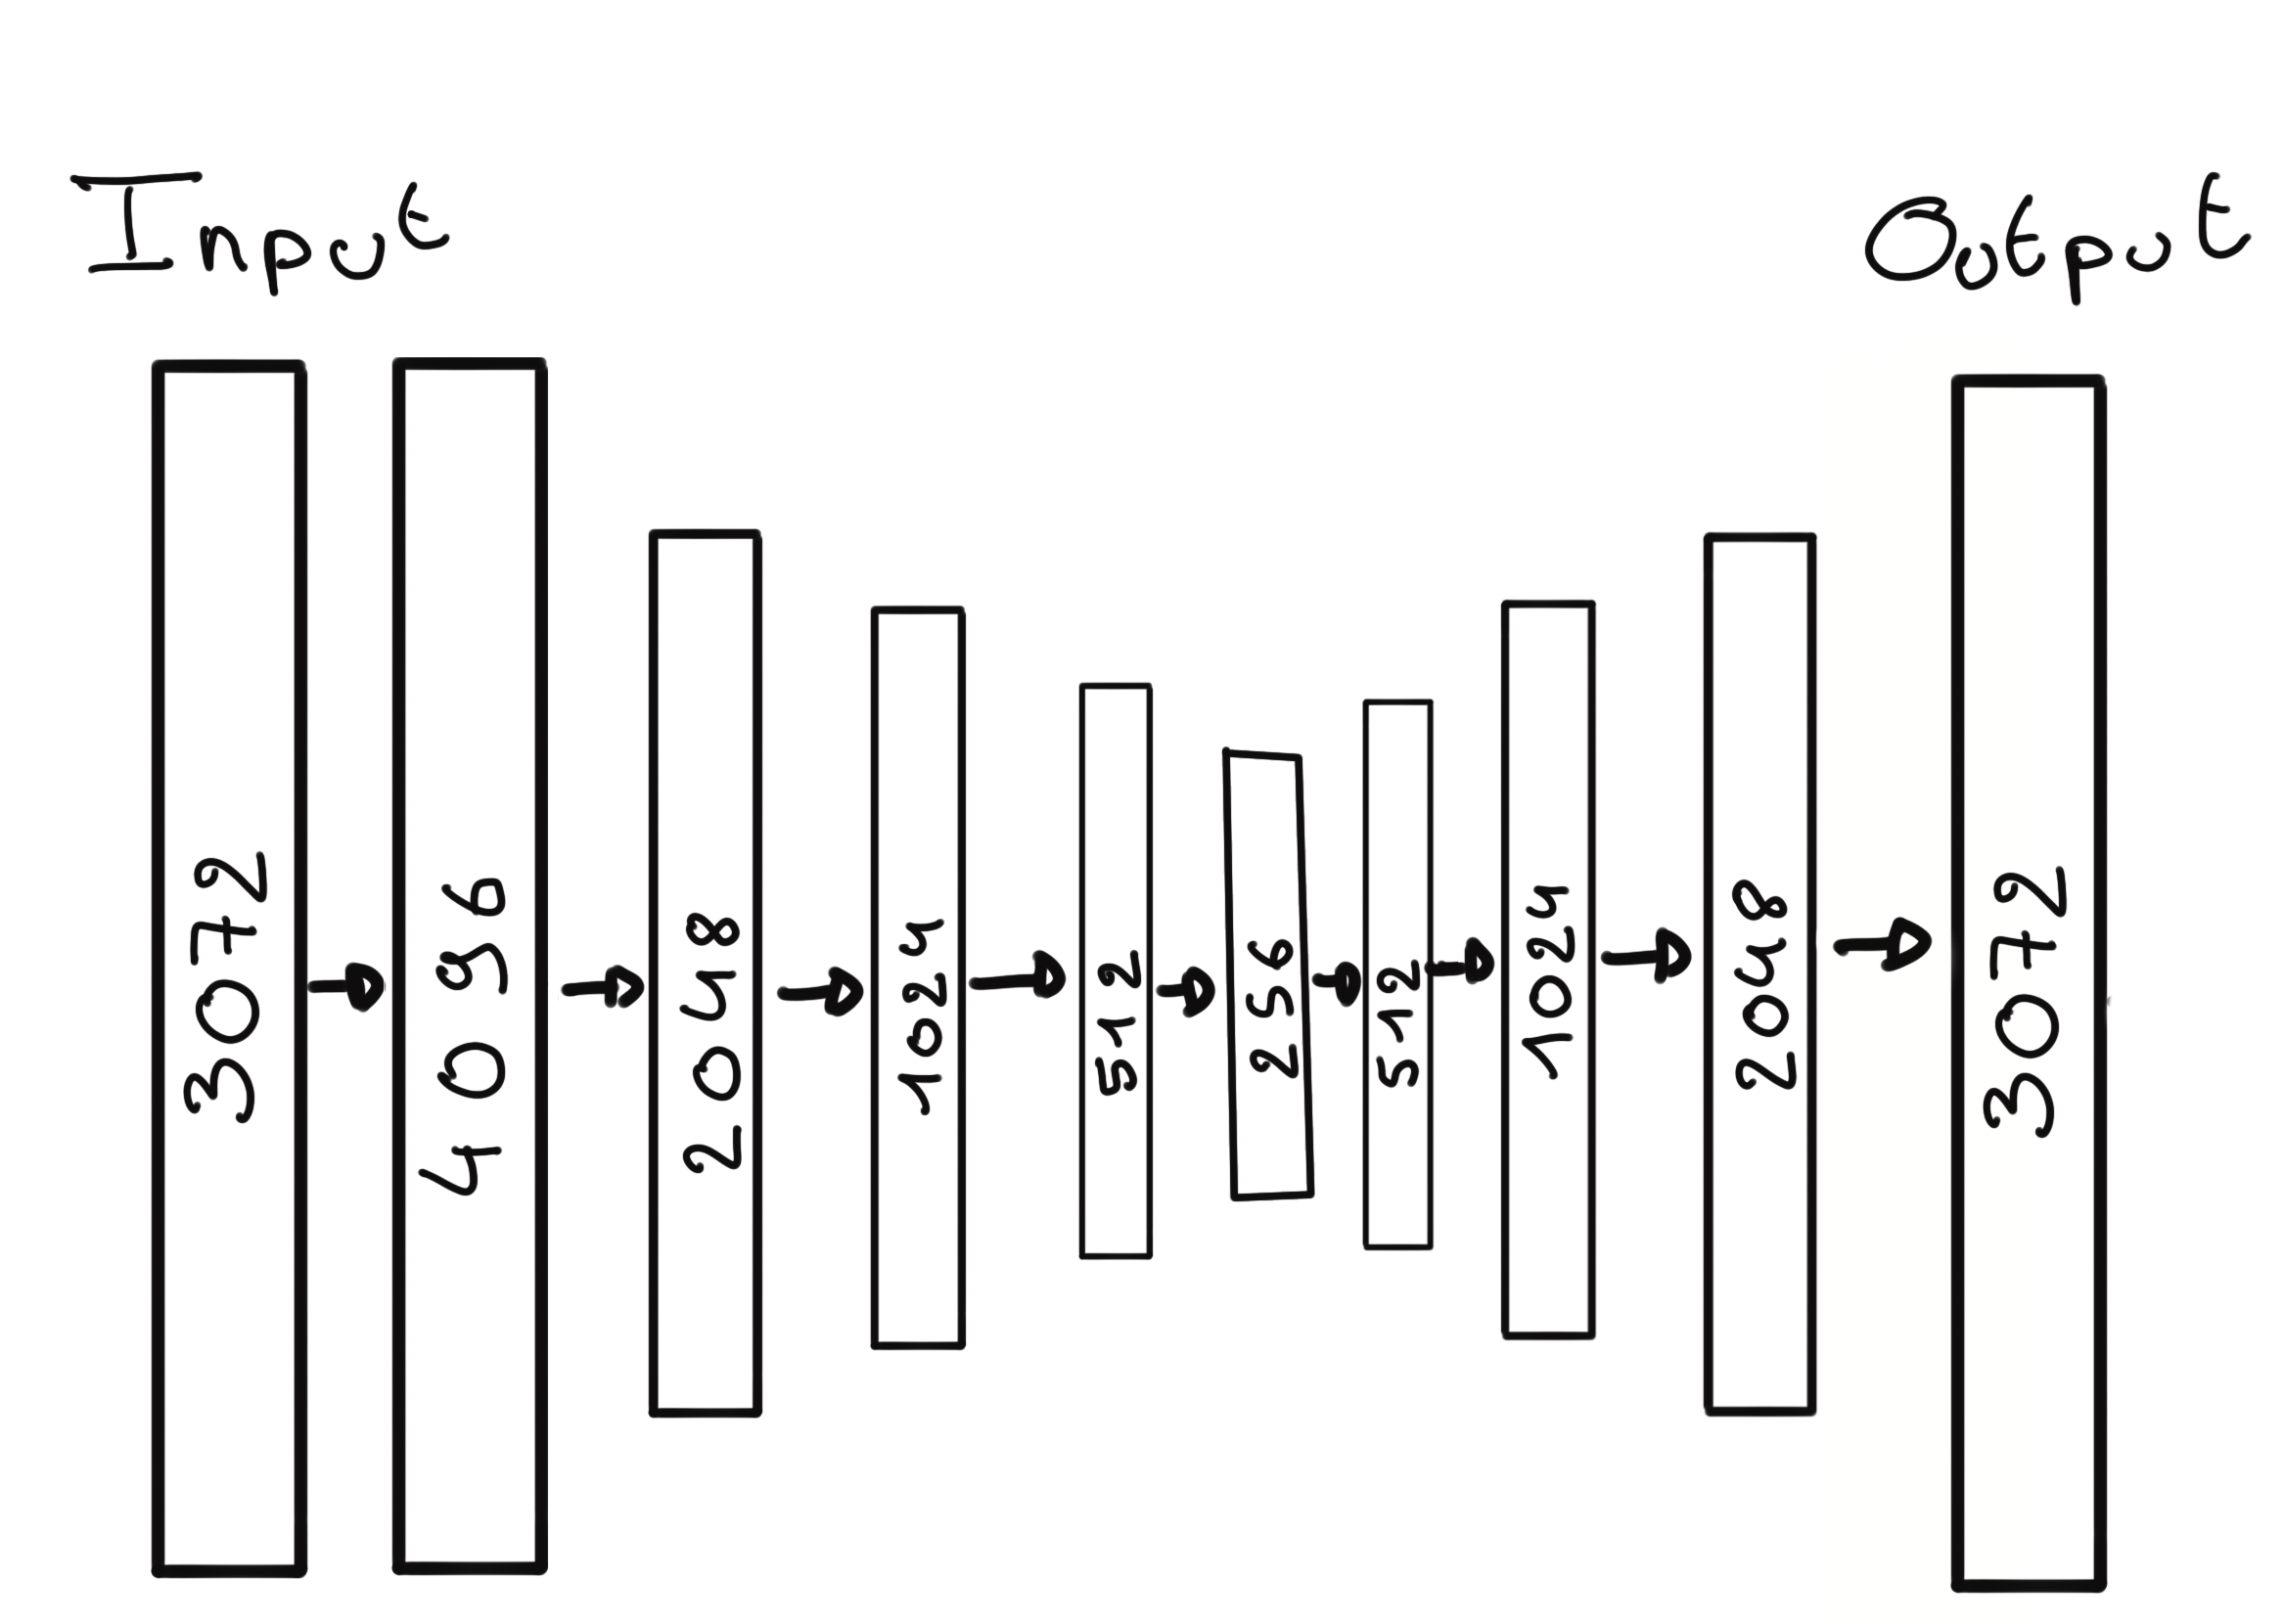
\includegraphics[height=6cm]{images/janne/ANN_illustration.png}
  \caption{Illustration of the ``bottleneck'' architecture of the ANN. Each block represent a fully connected layer with, on the left, the input layer and on the right the output layer. We see a first reduction of the number of neurons per layer, going from 4096 to 256, followed by an augmentation back to 4096 neurons, thus the ``bottleneck''.}
  \label{fig:janne:ann_arch}
\end{figure}

The idea behind this architecture is that, by reducing the number of neurons per layer, we force the network to summarize the event in 256 parameters, that it will use to regenerate an event. This architecture has also the advantage of keeping the number of learnable parameters relatively small, as the connection between small layers do not require a lot of parameters.

\subsubsection{ANN loss}

As it was mentioned in the introduction of Section \ref{sec:janne:arch}, the loss of the ANN is composed of two losses, the adversarial loss ${\cal L}_{adv}$ and the regularization loss ${\cal L}_{reg}$. To those two losses, we adjoin a penalty term that prevent the ANN from producing non-physical events.
\begin{equation*}
  {\cal L} = {\cal L}_{adv} + {\cal L}_{reg} + P
\end{equation*}

The adversarial loss ${\cal L}_{adv}$ is defined as the absolute value correlation between the reconstructed energy and the energy deposit (Eq. \ref{eq:janne:ladv}). The regularization loss ${\cal L}_{reg}$ is the MSE of the true and reconstructed energy position vector $(x, y, z, E)$ (Eq. \ref{eq:janne:lreg}).

The penalty term is here to prevent the network from generating event that are too far from the initial event. The relevance of this term and its parameters will be further discussed in Section \ref{sec:janne:arch:training}. The penalty $P$ is a function that takes the pixelated event $X$, its transformation after the ANN ${\cal G}(X)$ and a constraint $\epsilon$
\begin{equation}
  P(X, {\cal G}(X), \epsilon) = \sum_{i=1}^{3072} \left( ReLU(-{\cal G}(X)_i) + D_i \right)
\end{equation}
with
\begin{equation}
  D_i = \begin{cases}
    \frac{(X_i - {\cal G}(X)_i)^2}{X_i^2}& \text{if } \frac{|X_i - {\cal G}(X)_i|}{X_i} > \epsilon \\
    0& \text{otherwise}
  \end{cases}
\end{equation}
where $i$ index the HealPix pixels. The term $ReLU(-{\cal G}(X)_i$ is minimal, equal 0, when the charge after perturbation is positive. This term prevents the ANN from producing negative charge, feat impossible for the PMTs.

The second term $D_i$ is equal to 0 when the relative charge between the original and perturbed pixel is less than $\epsilon$. The value of $\epsilon$ will change during the training, as it will be explained in Section \ref{sec:janne:arch:training}. Otherwise, it is the square of this relative charge difference. This term penalizes the ANN from producing charges too different from the original event.
\hfill

When dealing with multiple losses like this, it is important keep then of the same order of magnitude, as we do not want one term to absorb the other.

The loss ${\cal L}_{adv}$ range from 0 to 1 while ${\cal L}_{reg}$ is 0 when the vertex and energy is perfectly reconstructed. It can theoretically go up to infinity. In practice, we expect it to take value of the order of magnitude coherent with the reconstruction performances. In fact, if it would take higher value, it would mean that the reconstruction would reconstruct the event far away from the true vertex and energy in comparison to the expected performance. This kind of issue would be immediately be detected, even with simplistic reconstructions such as the charge barycenter, which goes against the goal of producing subtle fluctuation.

We evaluate ${\cal L}_{reg}$ with $(x, y, z)$ in meter and $E$ in MeV. If the event is reconstructed with a precision of 15 cm and an energy resolution of 3\% at 1 MeV, taking the reconstruction performance of the best reconstruction algorithm OMILREC (see Sections \ref{sec:juno:reco} and \ref{sec:jgnn:results}), ${\cal L}_{reg} \approx 0.3^2 + 0.03^2 = 0.0909$. We see about an order of magnitude between ${\cal L}_{adv}$ and ${\cal L}_{reg}$. To compensate for it, we weight ${\cal L}_{reg}$
\begin{equation}
  {\cal L} = {\cal L}_{adv} + 60\cdot{\cal L}_{reg} + P(\epsilon)
\end{equation}

The amplitude of $P$ and the value of $\epsilon$ will be further discussed in Section \ref{sec:janne:arch:training}.

\subsubsection{Hyperparameter optimization}
%\label{sec:janne:arch:hyper}
%\begin{itemize}
%  \item Pour les meme raison que l'ANN:
%    \begin{itemize}
%      \item Phase exploratoire, architecture tres changeante, random search n'est pas viable
%      \item Architecture consomme beaucoup, besoin d'entrainer sur l'A100
%      \item Possiblement que de l'optimization permetterais de faire passer sur V100, mais developement techniques necessaires.
%    \end{itemize}
%\end{itemize}

All the ANN hyperparameters presented above have been optimized through the numerous iteration the architecture went through. The training is computationally expensive as we need to host both networks on the GPU card, reaching quickly the memory limit of the GPU. The training of the ANN can take up to 90 h. The requirement of having a powerful GPU can be met locally, as Subatech possess an available A100 \cite{noauthor_nvidia_nodate-1} card with 40 GB of memory. We could not port over computing center as they only possess V100 \cite{noauthor_nvidia_nodate-2} GPU with 20 GB of memory.

Those constraints made a random search optimization impossible. It is maybe possible, through optimization, to reduce the memory requirements to reach the threshold to run on V100 but the challenge was deemed not worth it for an exploratory work.

\subsection{Training of the ANN}
\label{sec:janne:arch:training}
%\begin{itemize}
%  \item Presentation du dataset
%  \item 2 etapes d'entrainement
%  \item Retour à l'identitié -> que l'ANN ne fasse pas n'importe quoi
%  \item Cassage de la reconstruction
%\end{itemize}

The ANN training is divided into two phases. In the first phase, the network learns to accurately reproduce physical events, ensuring that it can handle the intrinsic variability of the detector's response. This step is crucial, as it provides the foundation for the second phase, where the network searches for subtle perturbations that can degrade the reconstruction without being detected by standard calibration procedures. Splitting the training into two phases also allow saving a version of the network that know how to reproduce the physical events. We can then ``resume'' the training from this point if we just introduce changes in Phase 2, saving the training time of Phase 1.

For both phases, we use the both of the datasets presented in Section \ref{sec:janne:method}. We use a batch size of 64 for both datasets meaning that, for each step, the network see 128 events.

Each epoch go through the entirety of the training dataset.

\subsubsection{First training phase: back to physics}
\label{sec:janne:results:identity}

\begin{figure}[ht]
  \centering
  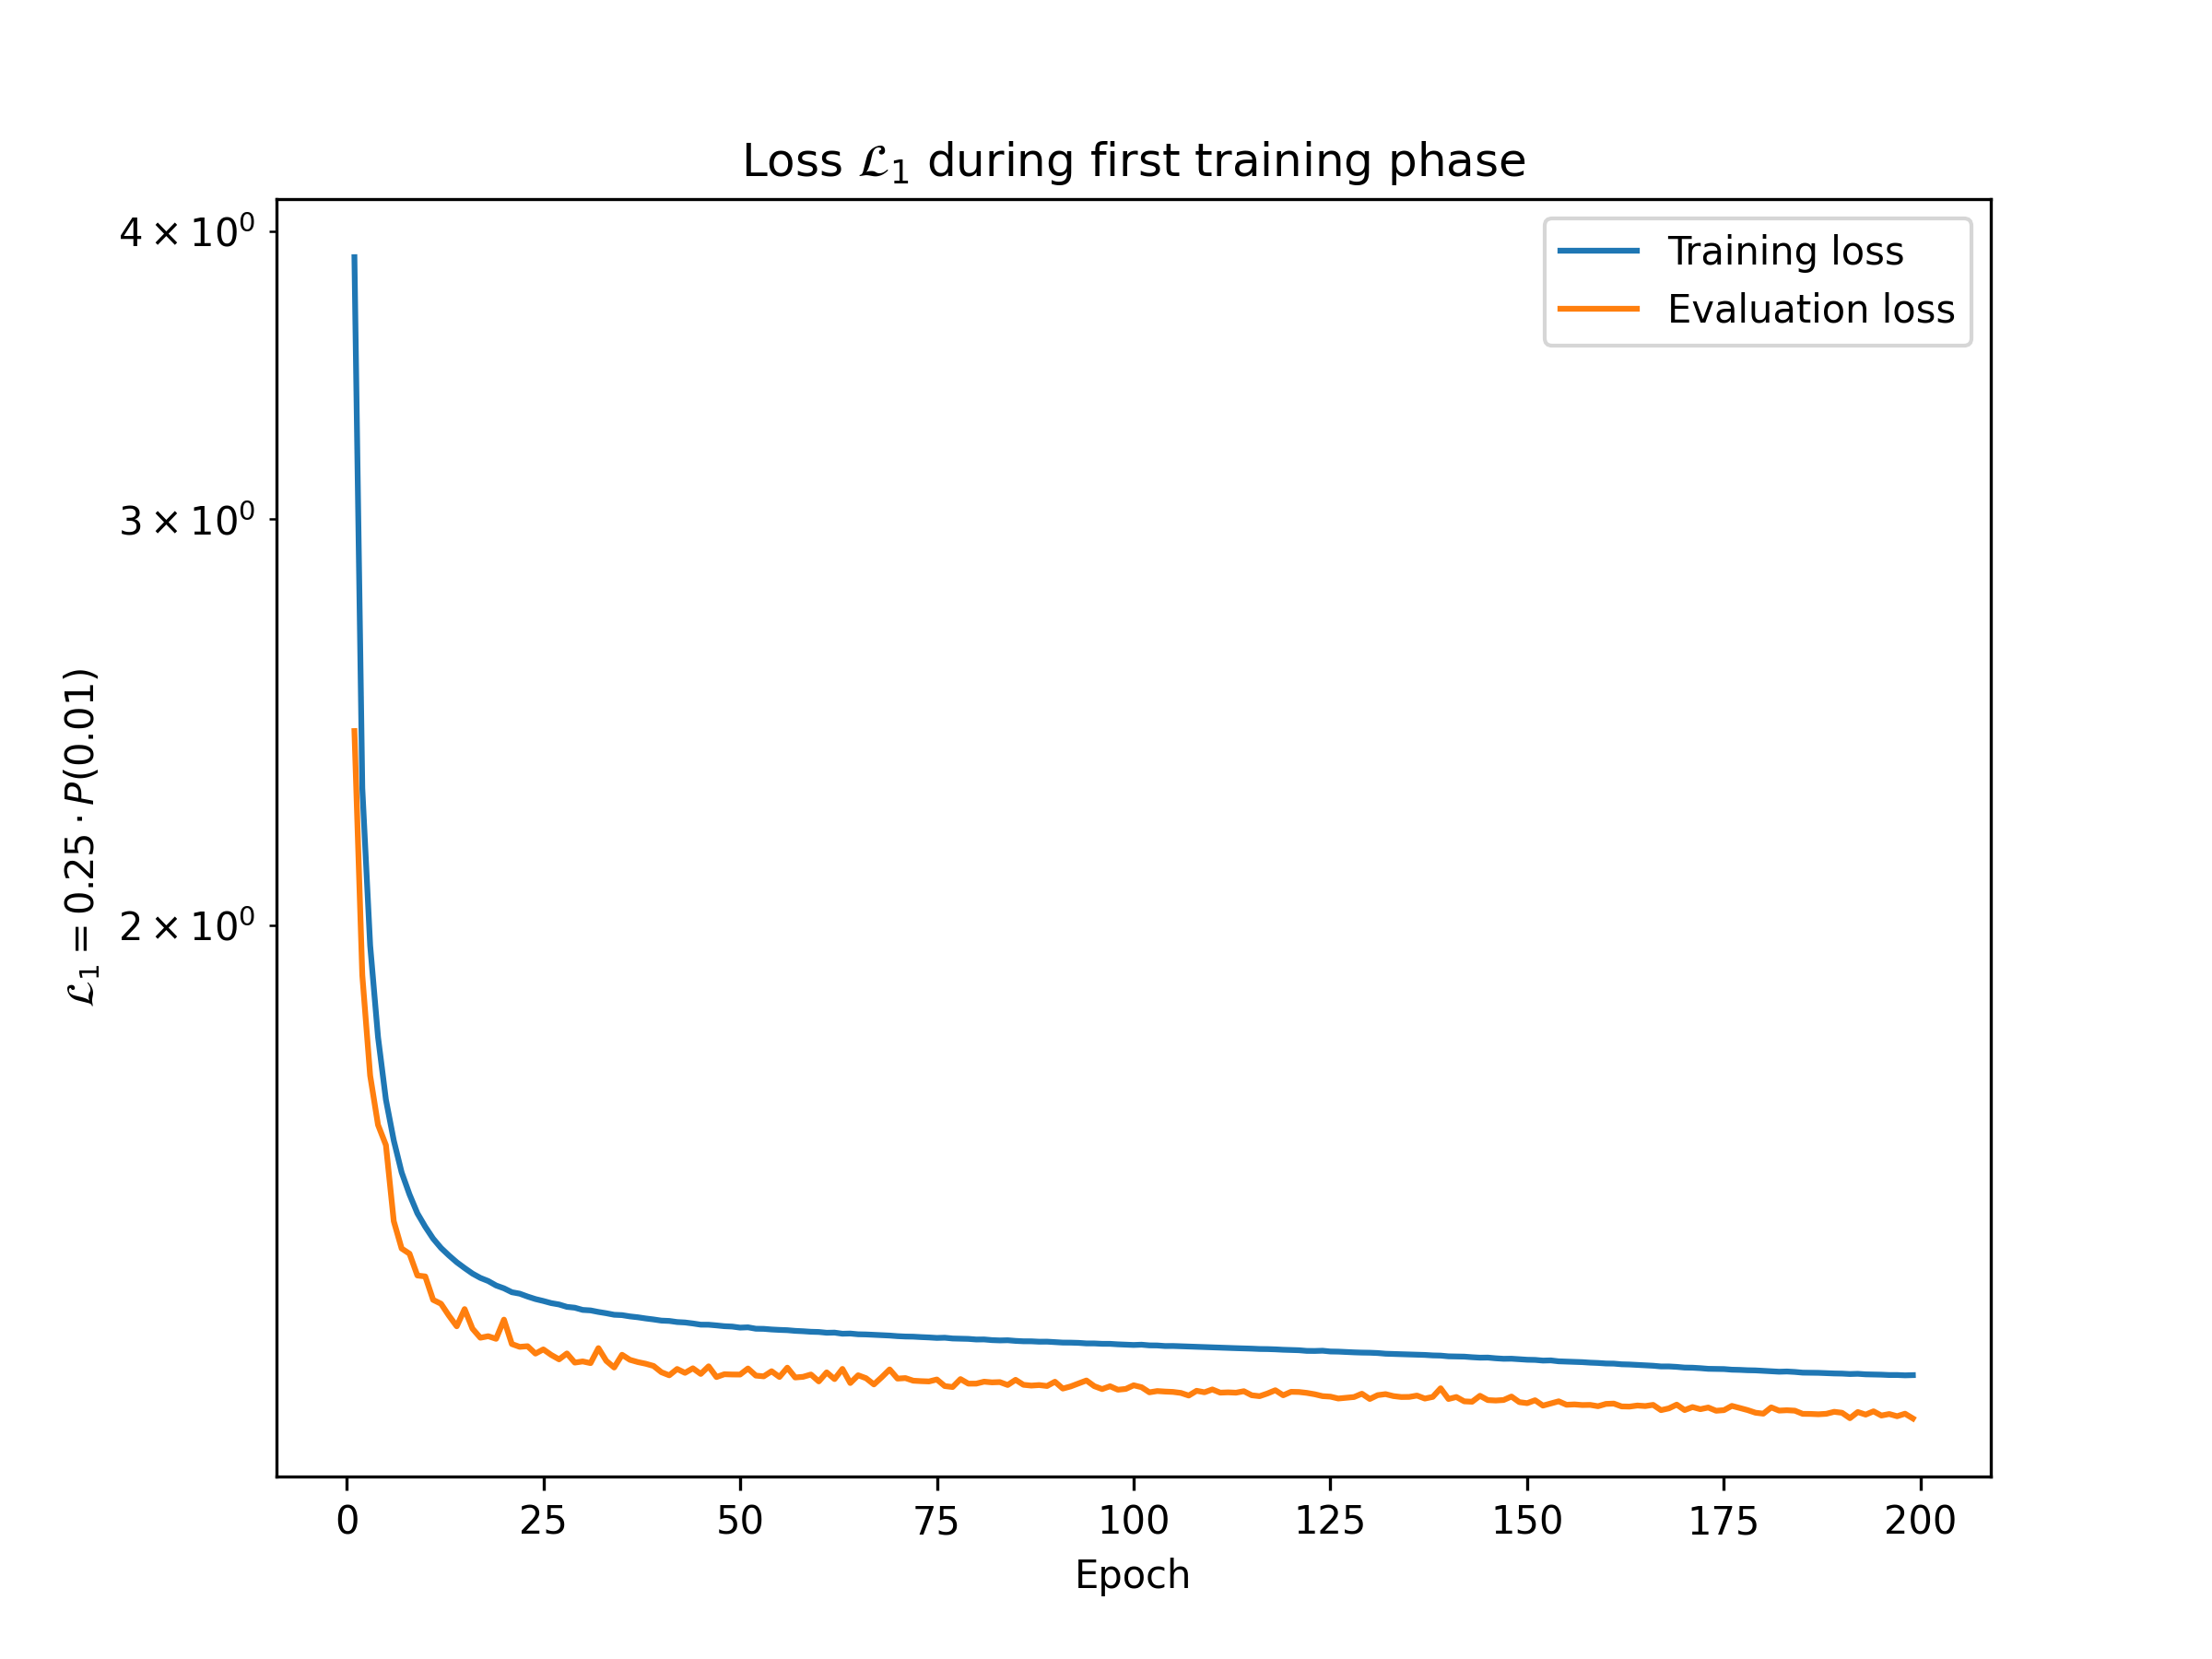
\includegraphics[height=6cm]{images/janne/training/phase_1_penal.png}
  \caption{Evolution of the loss ${\cal L}_1 = 0.25 \cdot P(0.01)$ during the first phase of the training.}
  \label{fig:jann:train:phase_1}
\end{figure}

When the ANN is initialized, before any training has been done, its parameters are initialized with random values. Multiple initialization methods exist. In this work, we use a common He initialization \cite{he_delving_2015}, which is the default initialization in the PyTorch \cite{ansel_pytorch_2024} library. If we were to ask for an event from the ANN without training first, the results would be random noise. We thus first have the ANN learn to reproduce physical events.

For this, we conduct a training of 200 epochs where the loss consists only of the penalty term. For scaling purposes, the penalty $P$ is scaled by 0.25.
\begin{equation}
  {\cal L}_1 = 0.25 \cdot P(\epsilon = 0.01)
\end{equation}
During this phase, the only objective of the network is to yield events that are the same as the original events.


The evolution of this loss ${\cal L}_1$ during the training for the training dataset and the validation dataset is presented in Figure \ref{fig:jann:train:phase_1}.
We see that the ANN converges to some stability in the loss.

The time and charge channels of two events, after this training phase, are presented in Figures \ref{fig:janne:hr_he_200} and \ref{fig:janne:lr_le_200}. We remind that the ANN only act on the charge channel of the event.
\begin{figure}[!ht]
  \centering
  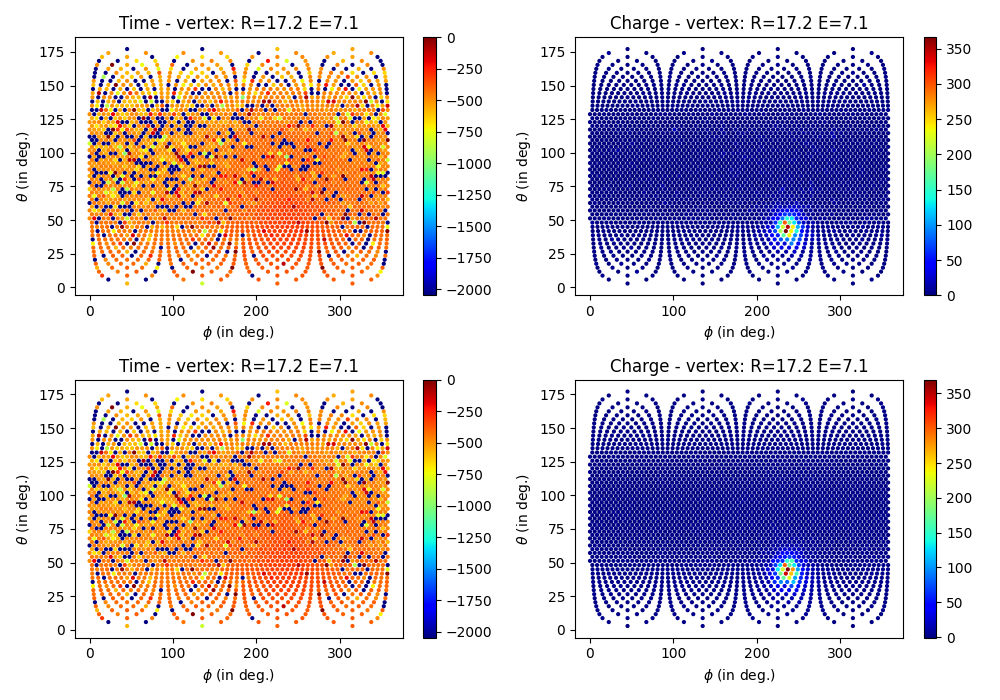
\includegraphics[height=7cm]{images/janne/events/hr_he_200.png}
  \caption{Time channel (on the left) and charge channel (on the right) of a \textbf{radial, high energy event} ($R$ = 17.2 m, $E_{dep}$ = 7.1 MeV), \textbf{Top:} before the ANN perturbation, \textbf{Bottom:} after the ANN perturbation. The ANN have been trained for 200 epochs, just after Phase 1. Time channel in ns and charge channel in $N_{pe}$.}
  \label{fig:janne:hr_he_200}
\end{figure}

\begin{figure}[!ht]
  \centering
  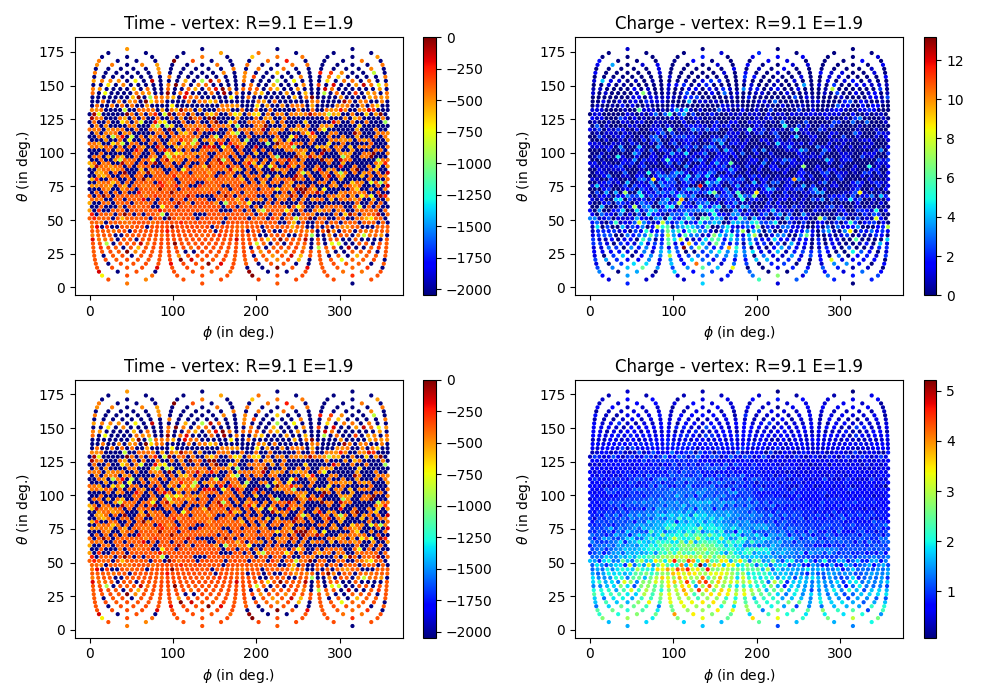
\includegraphics[height=7cm]{images/janne/events/lr_le_200.png}
  \caption{Time channel (on the left) and charge channel (on the right) of a \textbf{central, low energy event} ($R$ = 9.1 m, $E_{dep}$ = 1.9 MeV), \textbf{Top:} before the ANN perturbation, \textbf{Bottom:} after the ANN perturbation. The ANN have been trained for 200 epochs, just after Phase 1. Time channel in ns and charge channel in $N_{pe}$.}
  \label{fig:janne:lr_le_200}
\end{figure}

We observe that for a localized event, Figure \ref{fig:janne:hr_he_200}, the ANN correctly reproduces the event, while for a more diffuse event, Figure \ref{fig:janne:lr_le_200}, it produces a more uniform charge distribution. By looking at the color scale in Figure \ref{fig:janne:lr_le_200}, we observe that the ANN does not reproduce singular high numbers of $N_{pe}$. The highest pixel in the original was 12 $N_{pe}$, whereas after the ANN, the highest pixel is 5 $N_{pe}$. Furthermore, whereas in the original event the charge distribution, while diffuse, was still concentrated in specific pixels, the ANN spreads the charges in all the pixels.

In the next figures, we discuss the reconstruction of the FFNN (${\cal F}$) with and without the presence of the ANN $({\cal G})$ at the end of this Phase 1. The reconstruction by the FFNN of an event perturbed by the ANN is denoted $({\cal F} \circ {\cal G})$. We differentiate the reconstruction between the two datasets, presented in Section \ref{sec:janne:method}: the physics dataset, designated as IBD, and the control dataset, designated $^{12}B$.

In Figure \ref{fig:janne:f_circ_over_f_200}, we show the ratio between the reconstructed energy distribution before and after the application of the ANN. For the $^{12}$B dataset, the ratio is close to one except in the bin $E_{rec} > 9.5$ MeV, where we see an excess of events after the ANN. For the IBD dataset, the ratio is close to 1 over the energy range.

In Figure \ref{fig:janne:rec_err_200}, we present the distribution of the relative reconstruction errors $(E_{rec}, E_{dep})/E_{dep}$ with (light histogram) and without (dark histogram) the perturbations predicted by the ANN. We see that without the ANN, the distribution was centered on 0, whereas with it, we observe a small positive bias. In the second row of the histogram, the ratio between the light and dark histograms, we see confirmation of the previous observation, with a deficit of events for $-0.05 < (E_{rec}, E_{dep})/E_{dep}) < 0.02$ and an excess of events for $(E_{rec}, E_{dep})/E_{dep}) > 0.02$. This shift to higher energy explains the excess of events seen in the highest energy bins in Fig. \ref{fig:janne:f_circ_over_f_200}. The behavior between the $^{12}$B dataset (green histogram) and the IBD dataset (blue histogram) is similar.

At the end of this first reconstruction phase it's apparent that this exploratory ANN is not able to correctly reconstruct the event. This could come from the bottleneck architecture: the reduction of the event to 256 parameters is not enough to correctly rebuild the event. This subject will be further discussed in the conclusion of this chapter in Section \ref{sec:janne:conclusion}.

\begin{figure}[!ht]
  \centering
  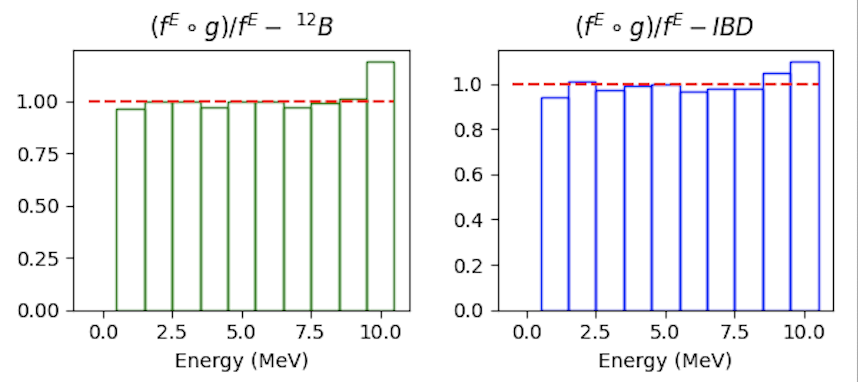
\includegraphics[height=4cm]{images/janne/f_circ_over_f_200.png}
  \caption{Ratio of the reconstructed energy spectra between $({\cal F} \circ {\cal G})$ and ${\cal F}$ at then end of Phase 1 of the training. \textbf{On the left :} For the $^{12}$B dataset. \textbf{On the right :} For the IBD dataset.}
  \label{fig:janne:f_circ_over_f_200}
\end{figure}

\begin{figure}[!ht]
  \centering
  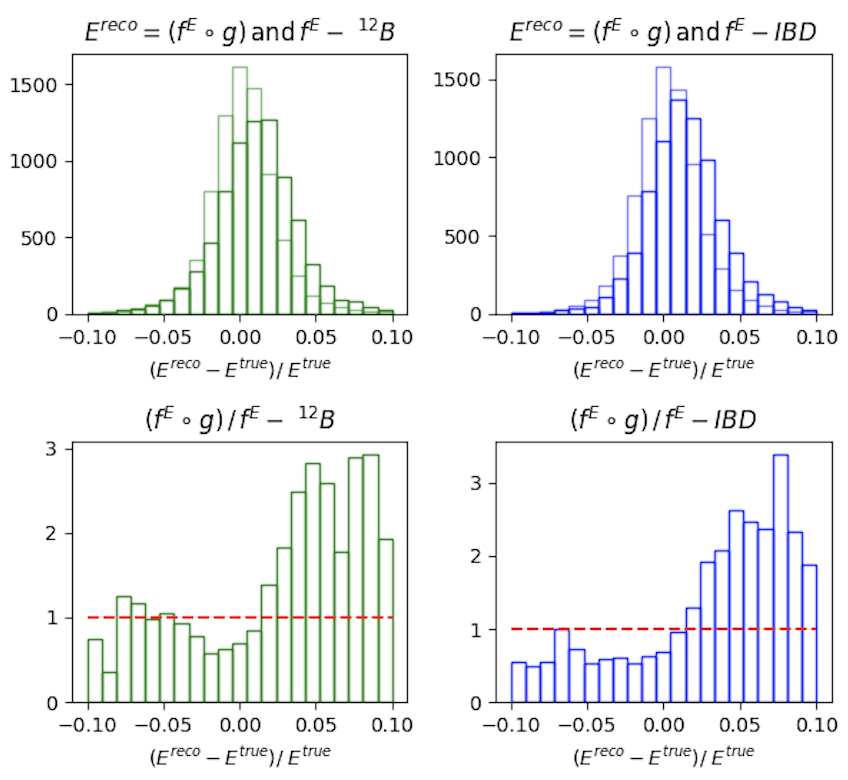
\includegraphics[height=8cm]{images/janne/rec_err_200.png}
  \caption{\textbf{On the top :} Distribution of the relative energy reconstruction error between ${\cal F}$ (light histogram) and $({\cal F} \circ {\cal G})$ (dark histogram) at then end of Phase 1 of the training. \textbf{On the bottom :} Ratio between the light and dark histogram of the top figure.}
  \label{fig:janne:rec_err_200}
\end{figure}


\subsubsection{Second training phase: Breaking of the reconstruction}
\label{sec:janne:results:break}

Once the ANN is able to reproduce physical events, we change the loss so that it starts to search for potential perturbations.
For this we introduce the term ${\cal L}_{adv}$ and ${\cal L}_{red}$ producing a second loss ${\cal L}_2$.
Adding those terms will significantly change the loss.
The previous minima in the parameter phase space the ANN found minimizing ${\cal L}_1$ will not be the minima ${\cal L}_2$. To prevent a gradient explosion, we introduce a growing factor $\lambda$ in front of the term ${\cal L}_{adv}$ and ${\cal L}_{red}$. This factor starts at $\lambda  = 0.01$ at epoch 201 and grows $\lambda_{i+1} = \lambda_{i} + 0.01$ where $i$ indexes the epoch. It caps at $\lambda_{max} = 1$ at epoch 300 after which it stops growing.

Also, to ease the task of the ANN, we relax the constraint in the penalty term $P$ from $P(0.01)$ to $P(0.15)$.

The expression of the phase 2 loss ${\cal L}_2$ becomes:
\begin{equation}
  \label{eq:janne:phase_2:loss}
  {\cal L}_2 = \lambda \left( {\cal L}_{adv} + 60 \cdot {\cal L}_{reg} \right) + 0.25 \cdot P(0.15)
\end{equation}


This second phase of the training last for 200 more epochs, up to epoch 400.

The profiles of ${\cal L}_2$, ${\cal L}_{adv}$, $60 \cdot {\cal L}_{reg}$ and $0.25 \cdot P(0.15)$ during this second phase of the training are presented in Figures \ref{fig:janne:phase_2_1} and \ref{fig:janne:phase_2_2}. The profile of the loss ${\cal L}$ over entirety of the training is presented in Figure \ref{fig:janne:phase_all}.

\begin{figure}[ht]
  \centering
  \begin{subfigure}[t]{0.48\linewidth}
    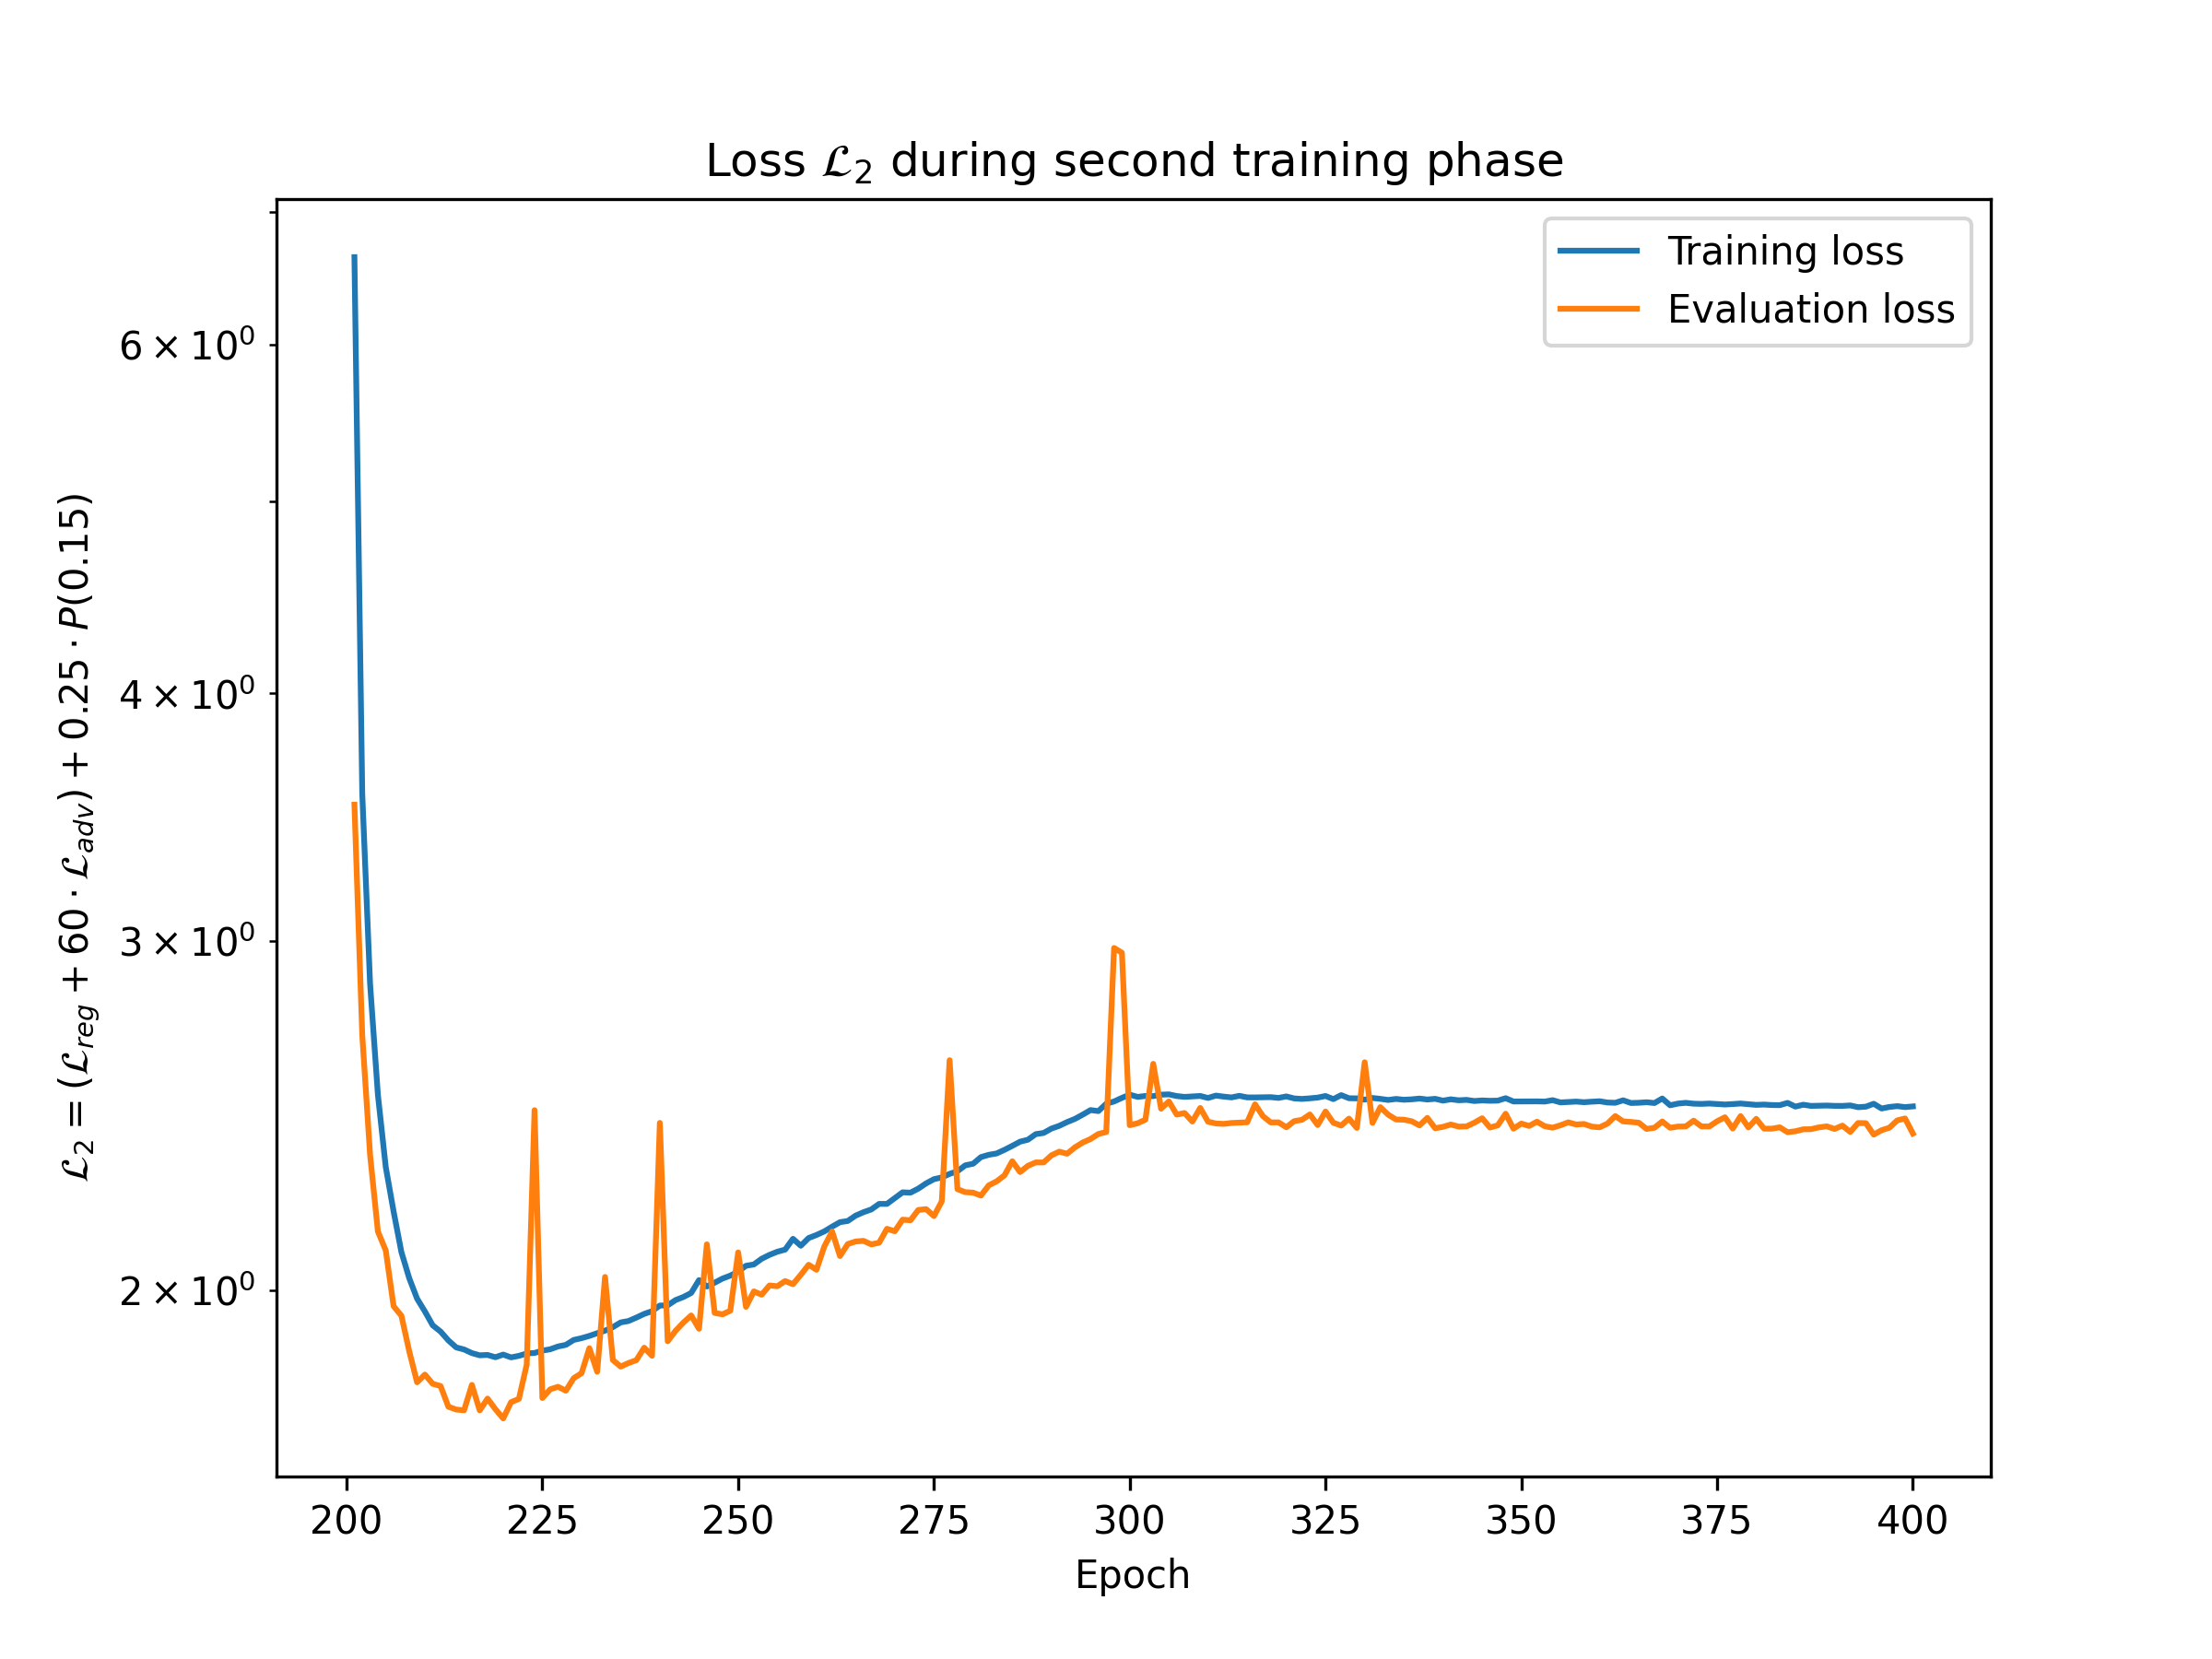
\includegraphics[width=\linewidth]{images/janne/training/phase_2_loss.png}
  \end{subfigure}
  \hfill
  \begin{subfigure}[t]{0.48\linewidth}
    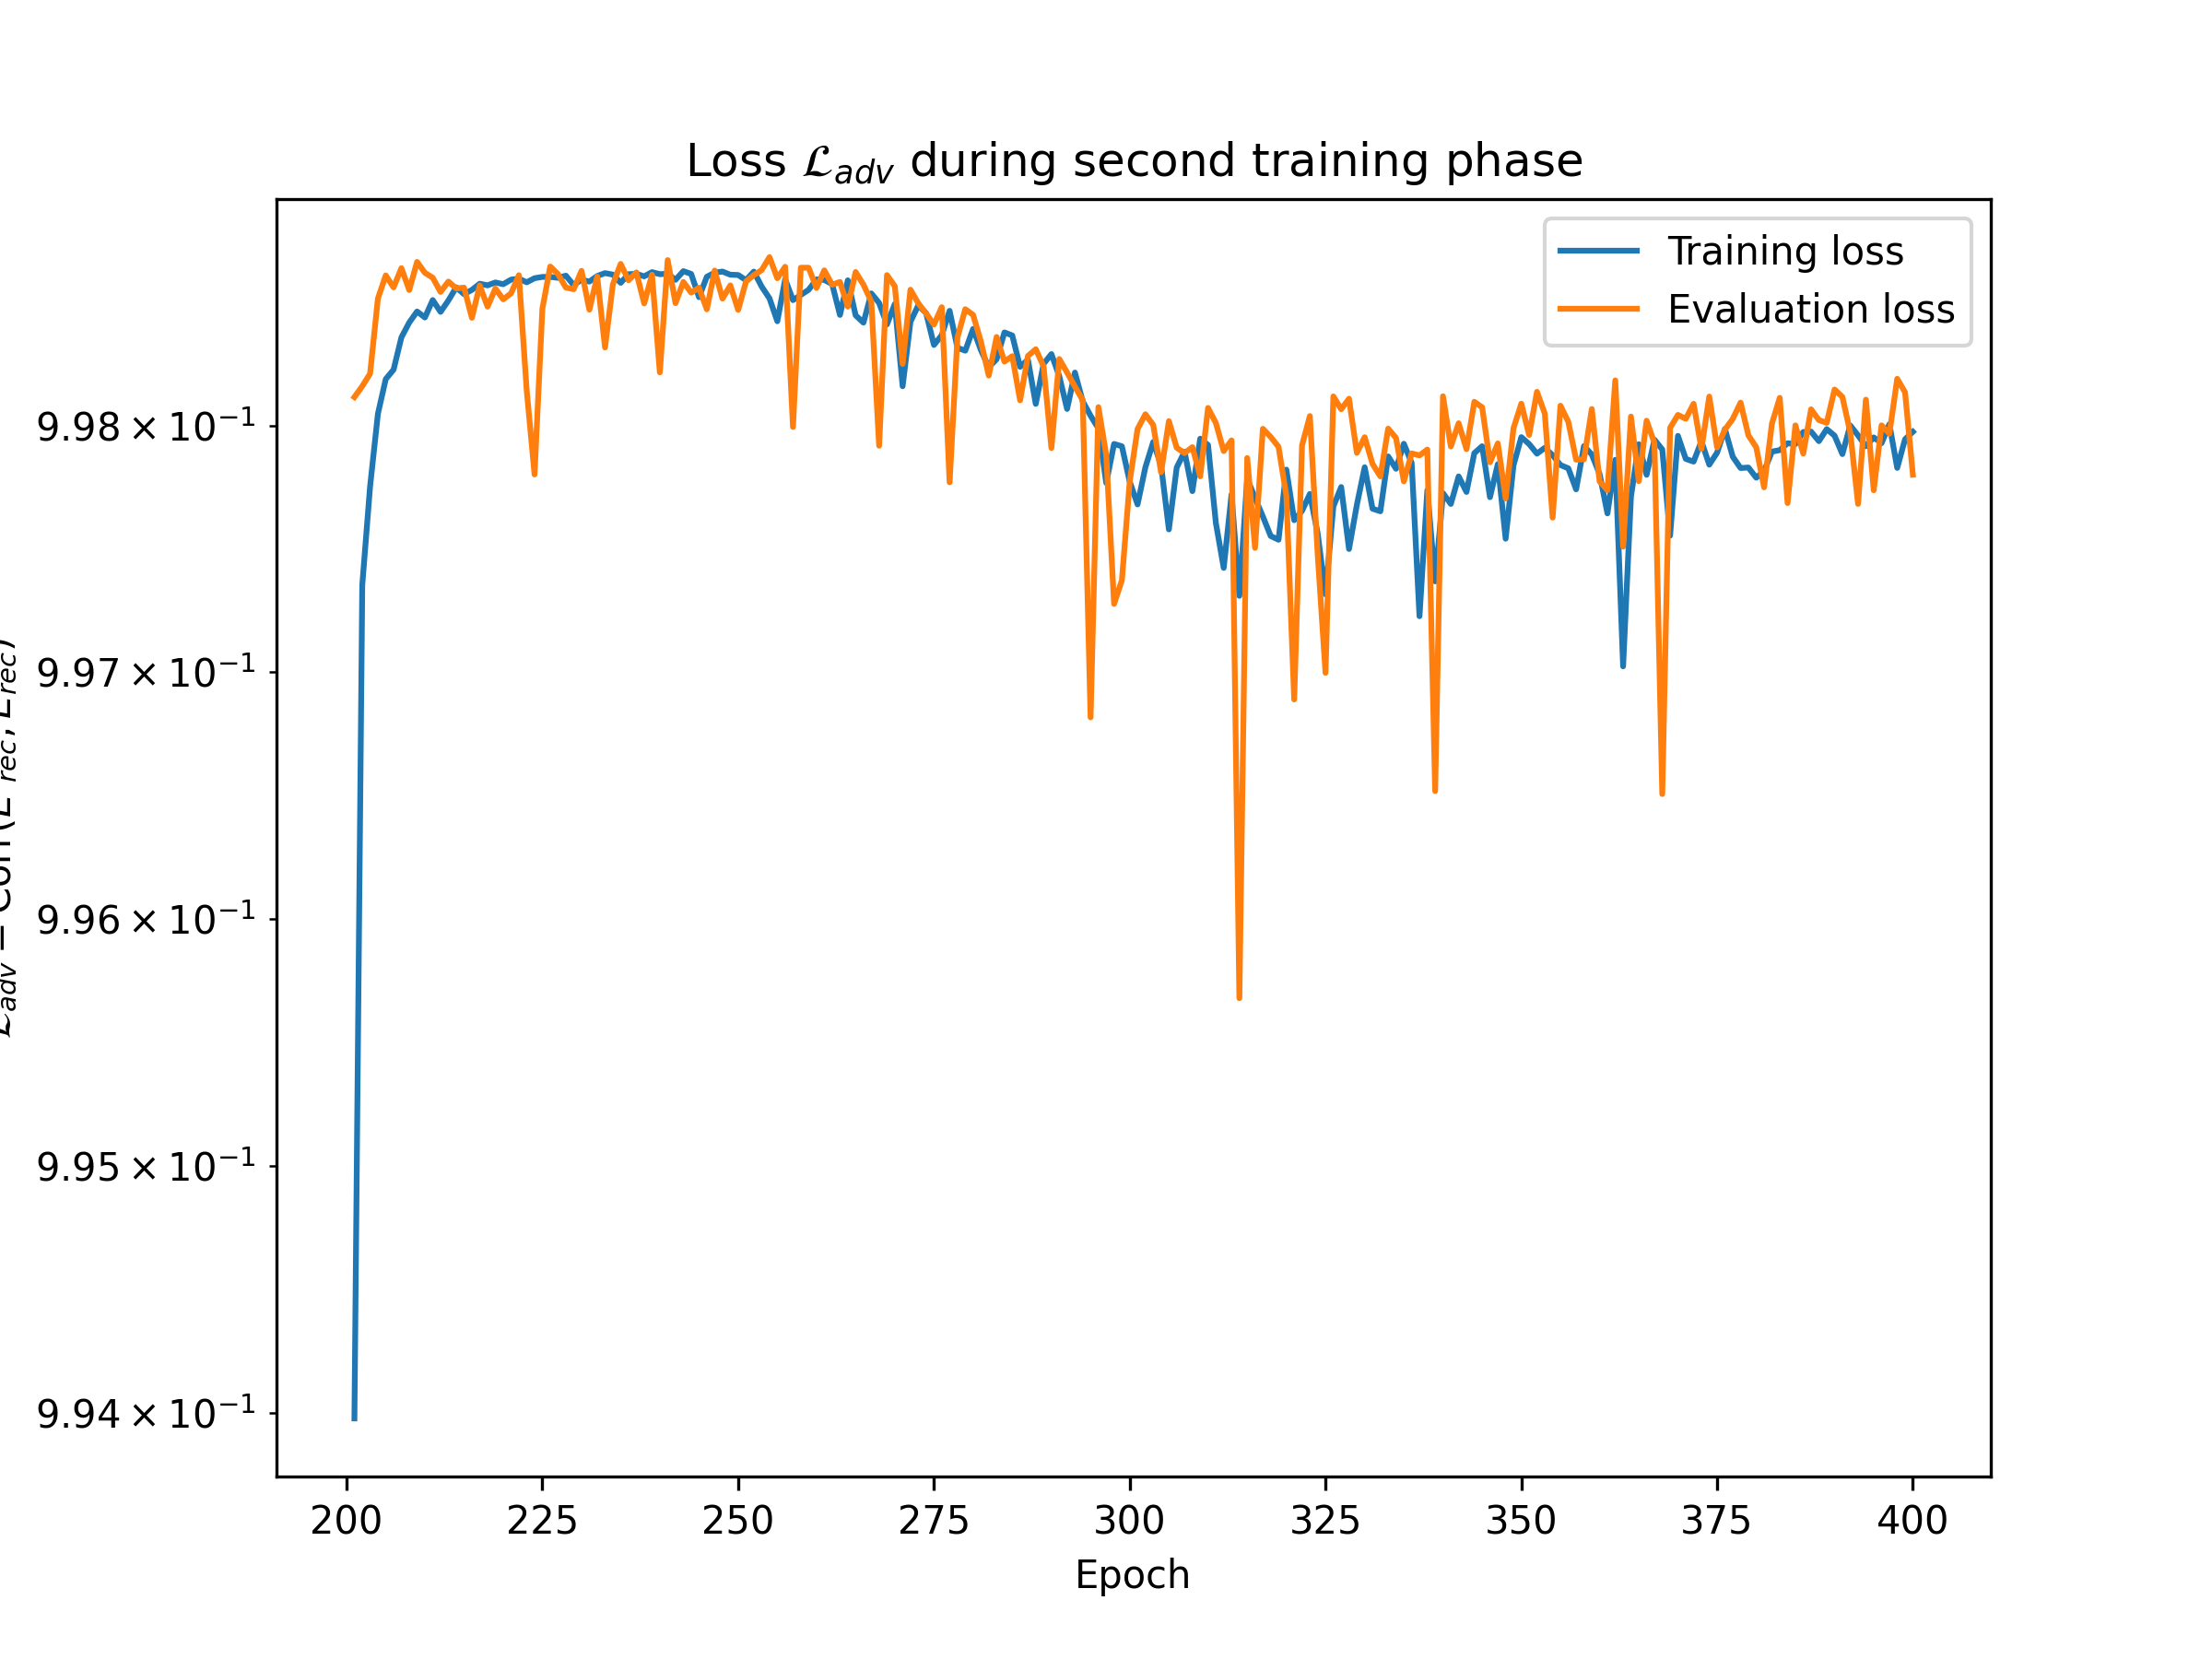
\includegraphics[width=\linewidth]{images/janne/training/phase_2_loss_adv.png}
  \end{subfigure}
  \caption{Profile of the loss ${\cal L}_2$ and ${\cal L}_{adv}$ during the second phase of training. The linear increase of ${\cal L}_2$ is due to the growing factor $\lambda$ in Eq. \ref{eq:janne:phase_2:loss}.}
  \label{fig:janne:phase_2_1}
\end{figure}

\begin{figure}[ht]
  \centering
  \begin{subfigure}[t]{0.48\linewidth}
    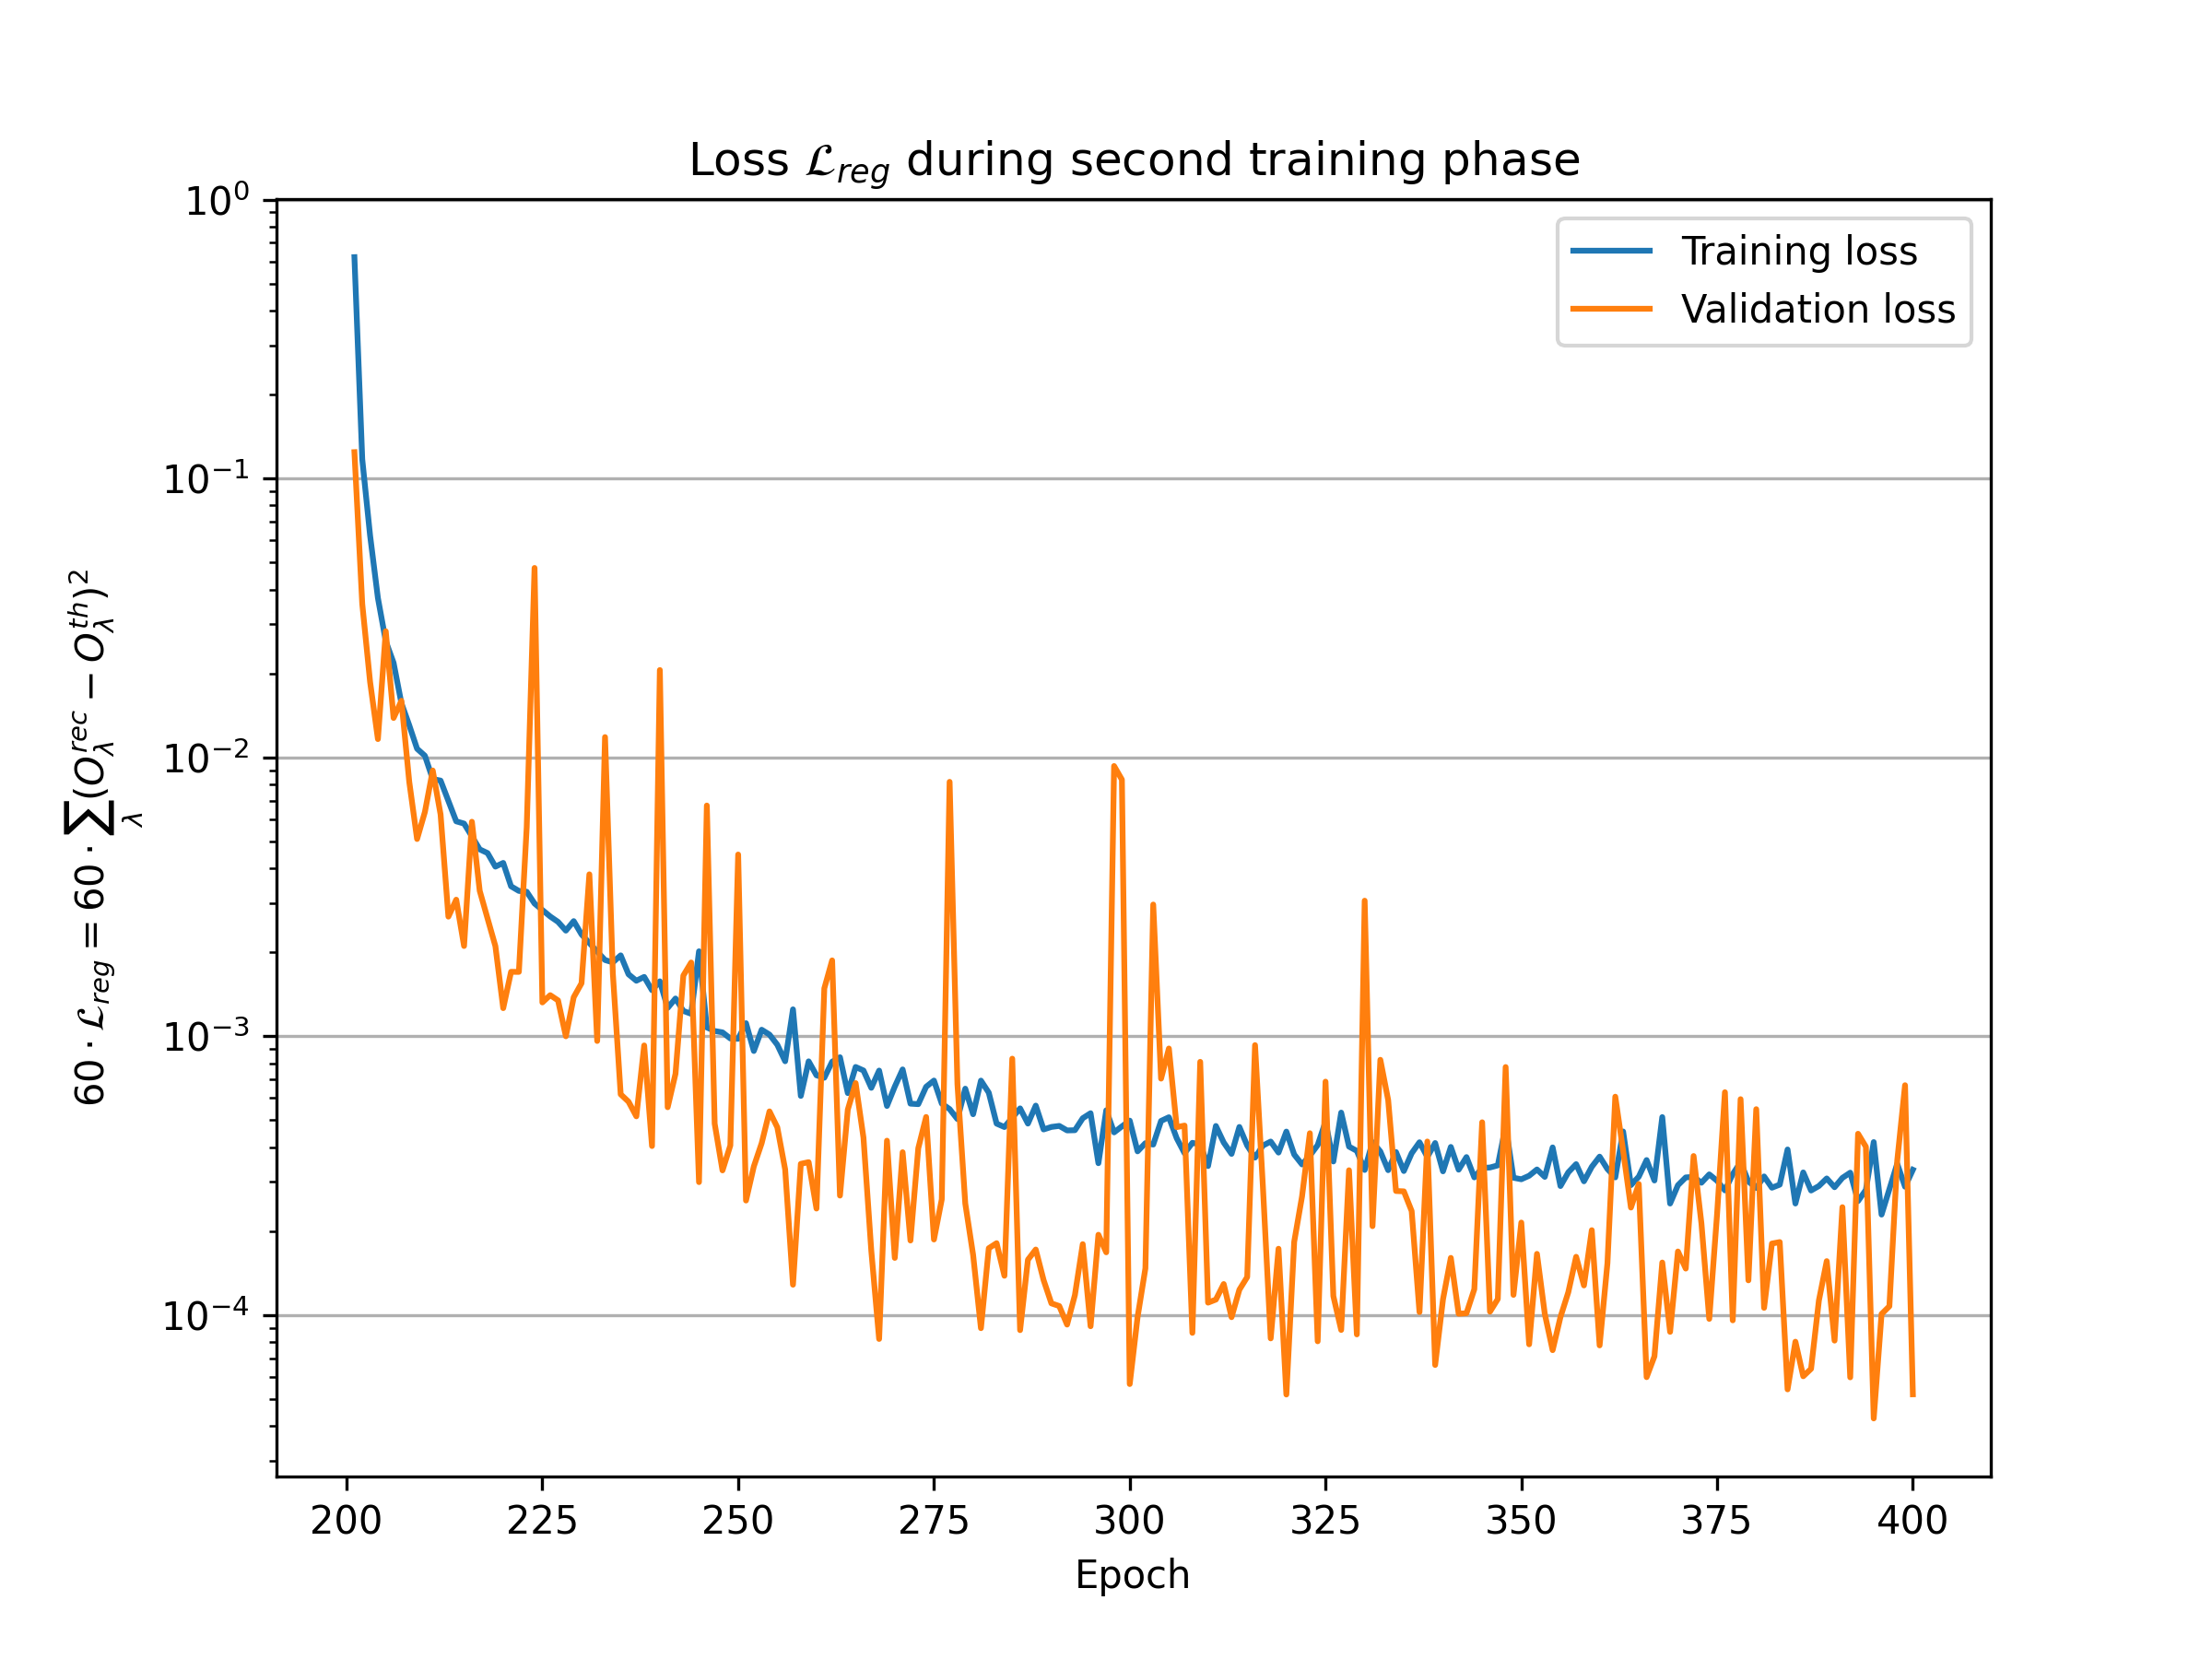
\includegraphics[width=\linewidth]{images/janne/training/phase_2_loss_reg.png}
  \end{subfigure}
  \hfill
  \begin{subfigure}[t]{0.48\linewidth}
    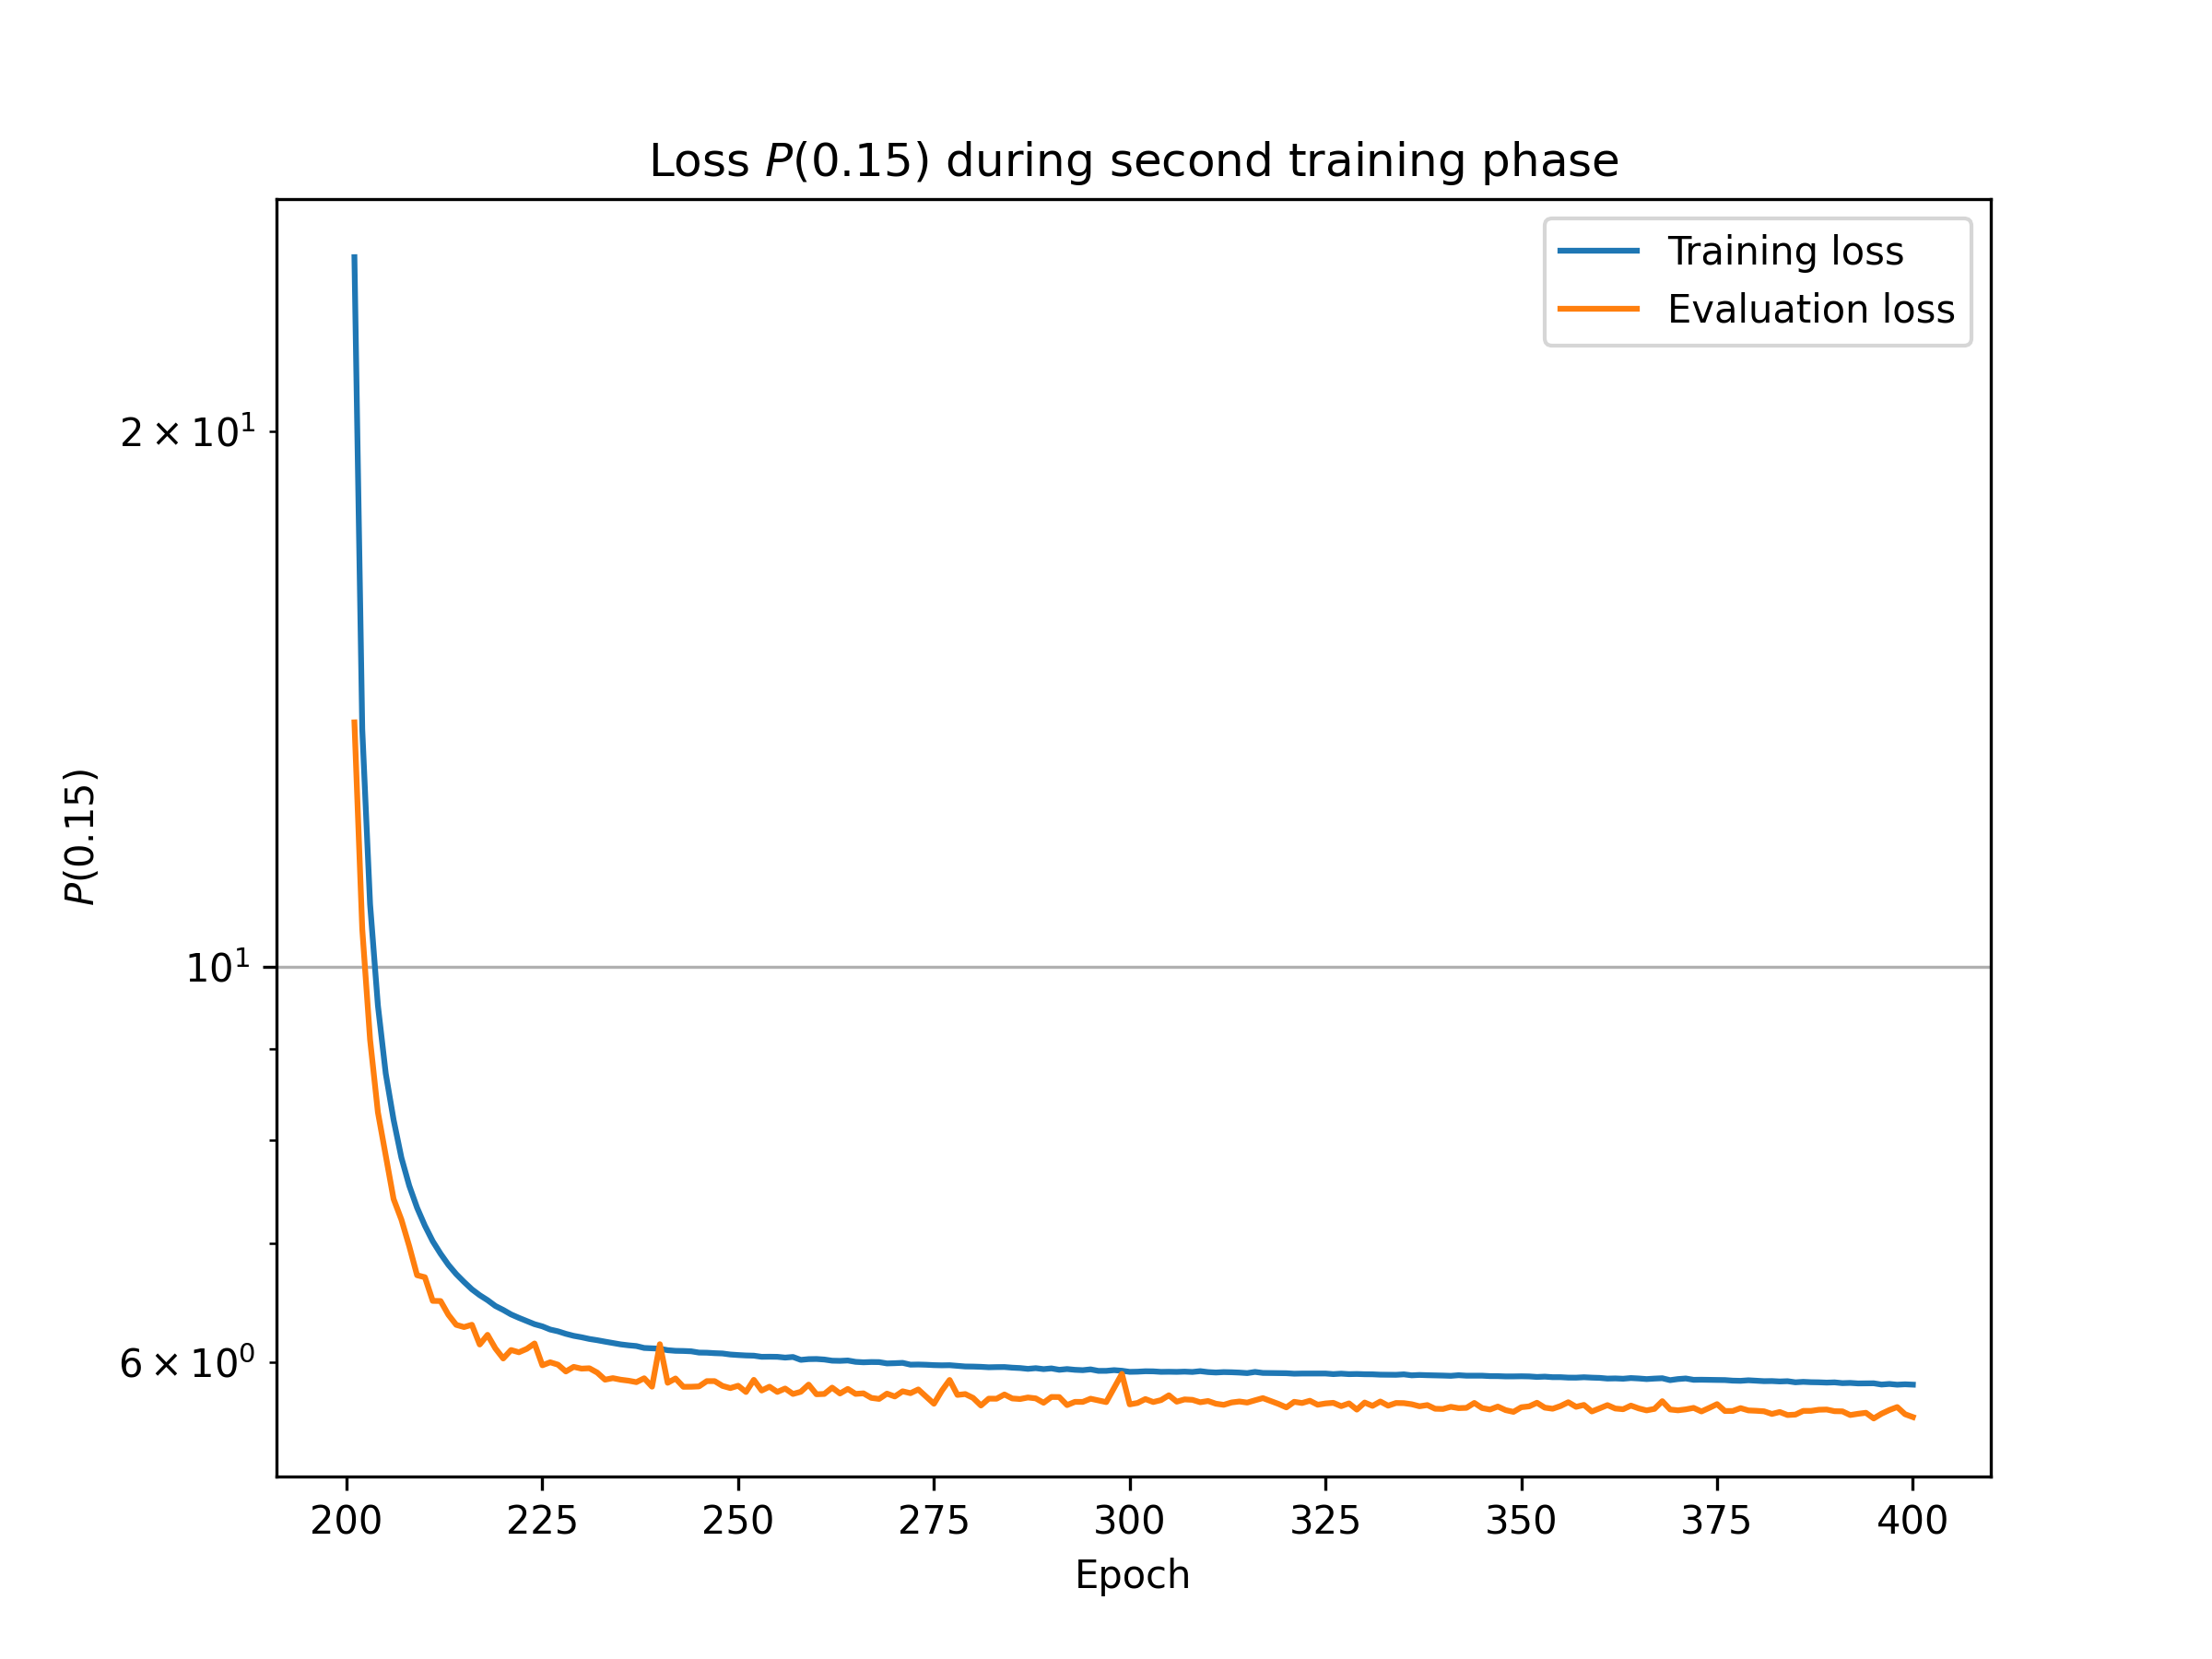
\includegraphics[width=\linewidth]{images/janne/training/phase_2_penal.png}
  \end{subfigure}
  \caption{Profile of the loss $60 \cdot {\cal L}_{reg}$ and $0.25 \cdot P(0.15)$ during the second phase of training.}
  \label{fig:janne:phase_2_2}
\end{figure}

\begin{figure}[ht]
  \centering
  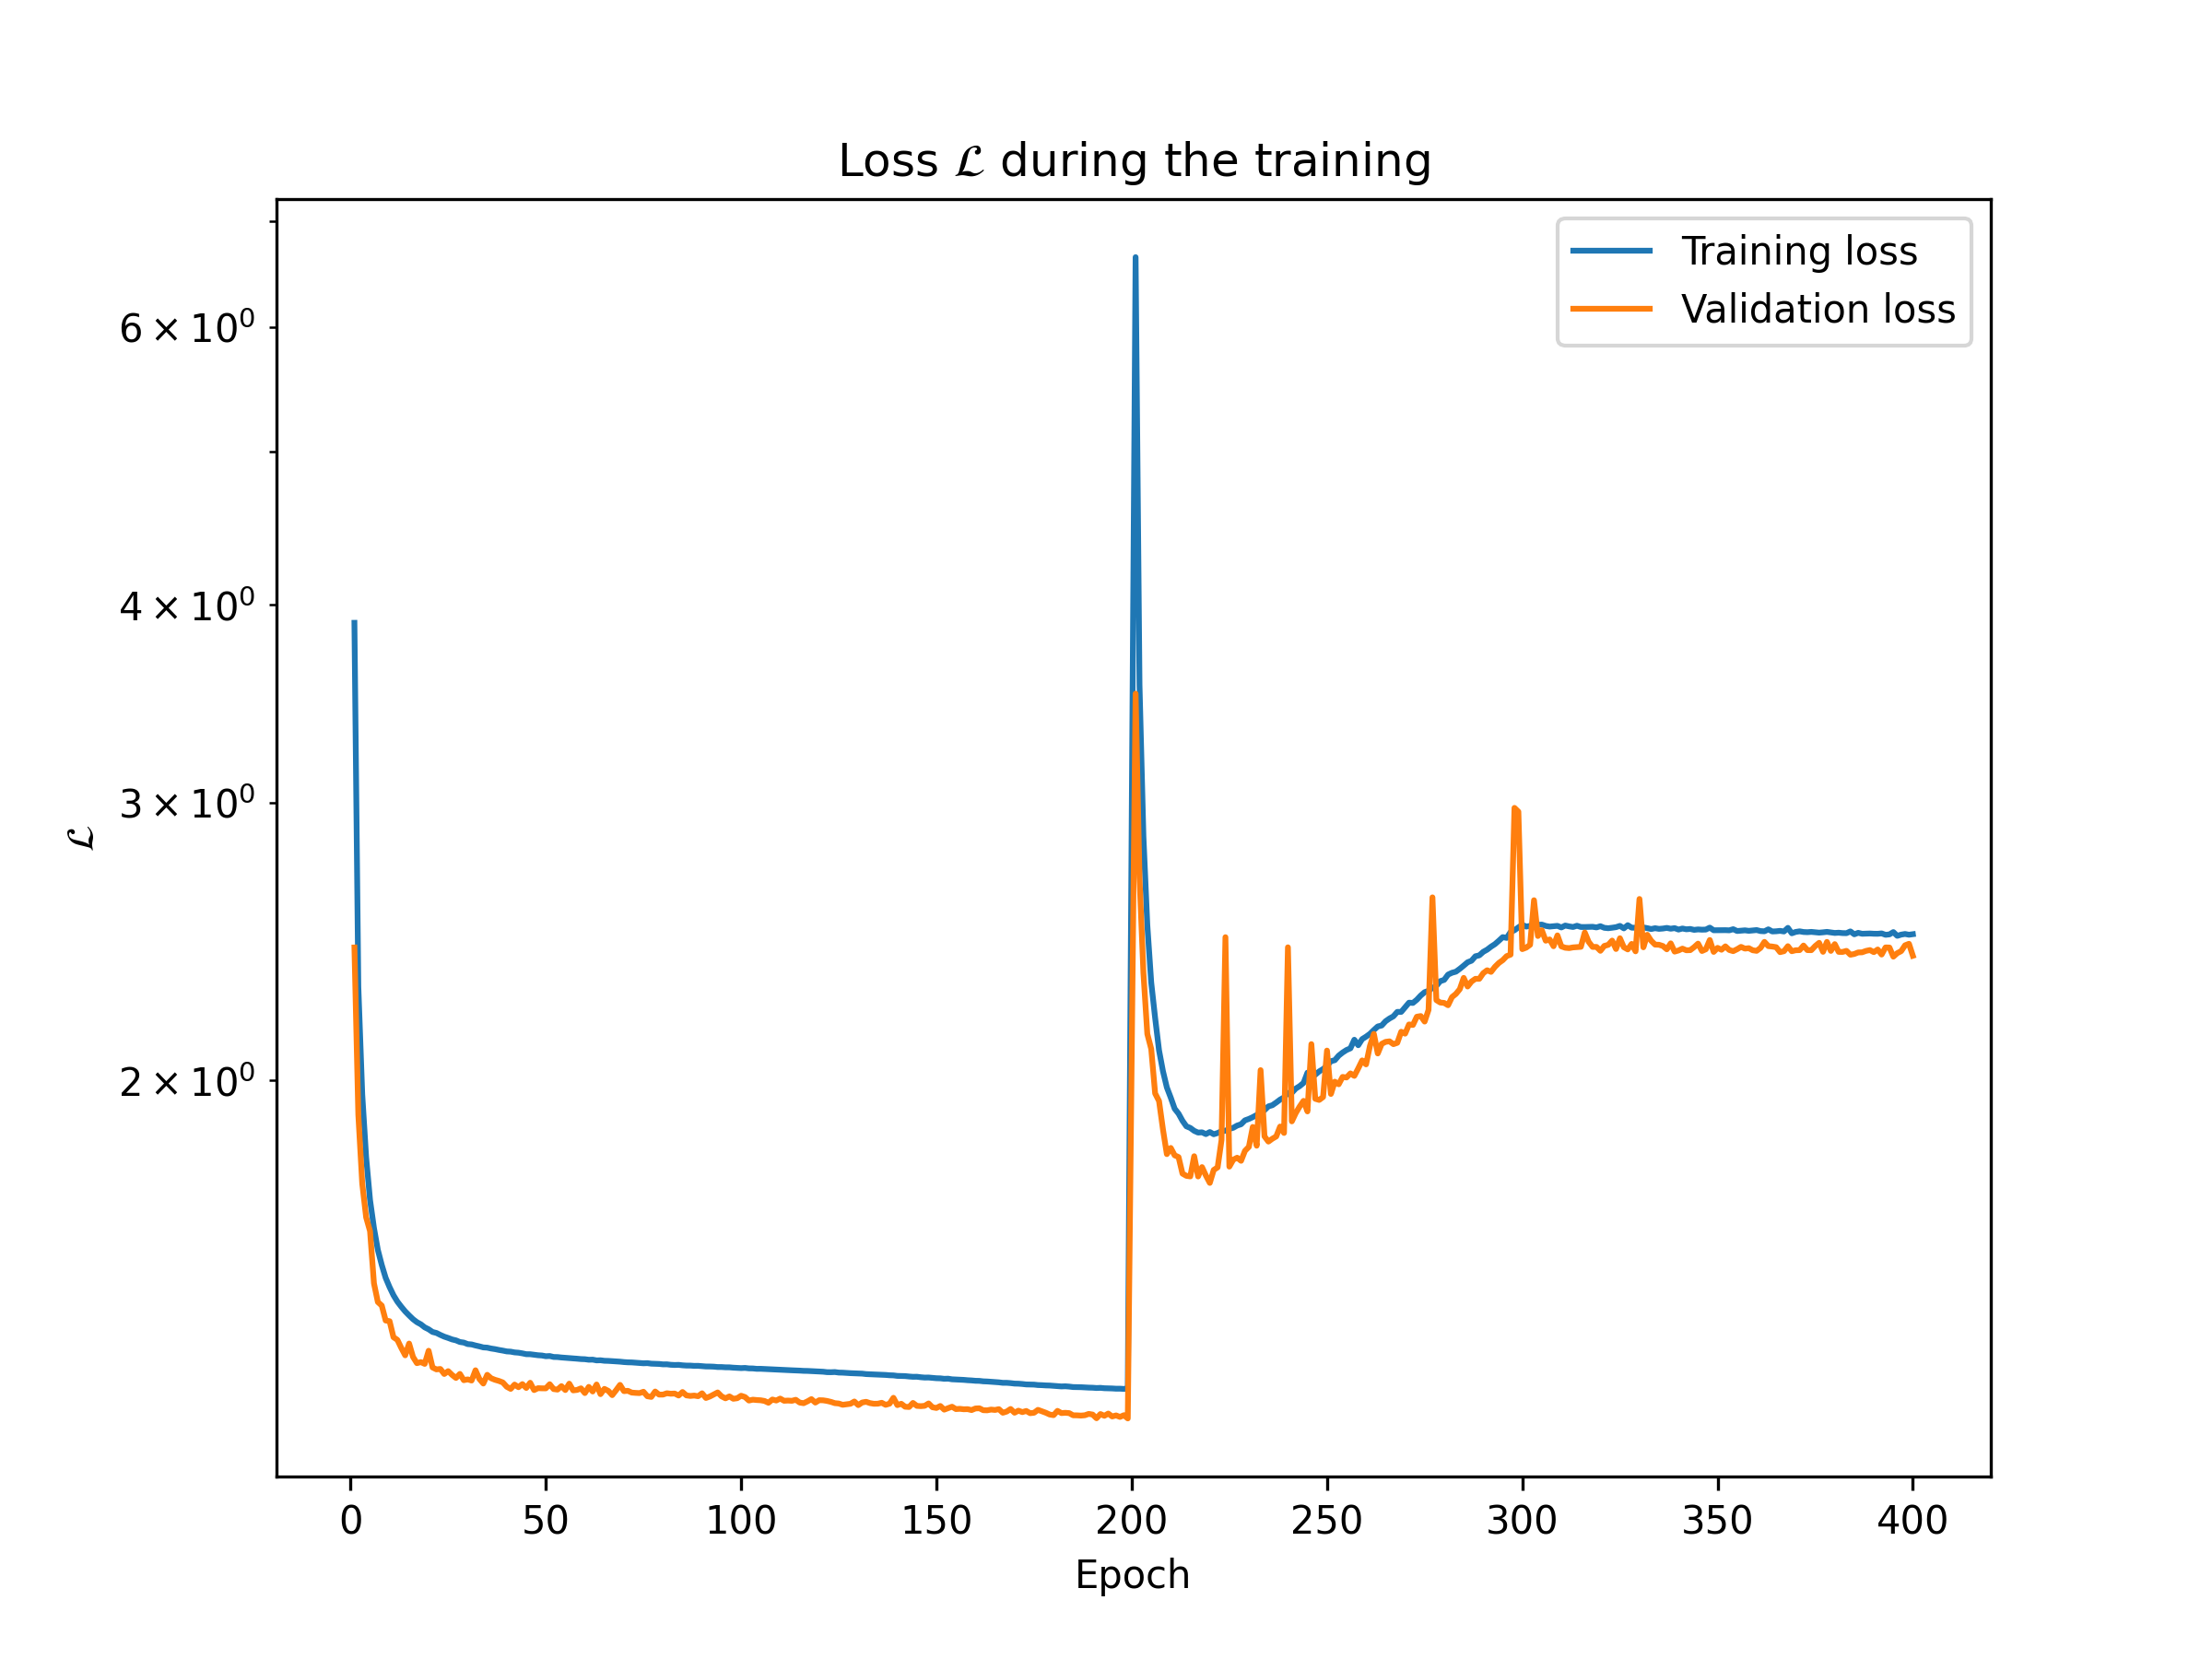
\includegraphics[height=6cm]{images/janne/training/phase_all_l.png}
  \caption{Profile of the loss over the entirety of the training (Phase 1 and 2).}
  \label{fig:janne:phase_all}
\end{figure}


We see on Figures \ref{fig:janne:phase_2_1} and \ref{fig:janne:phase_2_2} that during the first epochs of this second phase, $L_{reg}$ and $P(0.15)$ decrease fast. At the end of the 1st phase, the
work to recover the initial reconstruction seems incomplete since the performance of FFNN were not recovered (Fig. \ref{fig:janne:rec_err_200}). During the first epochs of the second phase, $L_{reg}$ seems to continue this work. This is logical since this term is suppose to temperate the perturbations so they are not visible with a control sample.  At the same time, we see a quick increase of $L_{adv}$, confirming that the reconstruction is less broken.

During most of the next 50 epochs of this phase, all losses are more stable before $L_{adv}$ starts decreasing, between epochs 250 and 300. It suggests $L_{adv}$  has managed to re-deteriorate the reconstruction, despite the quasi stability  (or slow decrease) of $L_{reg}$. This is the desired behavior concerning the losses.

Unfortunately, as can be seen in Figs. \ref{fig:janne:f_circ_over_f_400} and \ref{fig:janne:rec_err_200}, the performance of the reconstruction is still too deteriorated: it would very probably be detected by data/MC comparisons with control samples. Also, on these figures and on Figure \ref{fig:janne:ann_effect_400}, we can't see an indication that IBD events are affected more than $^{12}B$ events by the perturbation. A difference here is not mandatory: the same deterioration of the resolution could still be undetectable in data/MC comparison of the distributions of the energy or of the vertex position  in $^{12}B$ samples, and still be enough to alter the oscillation analysis. However, observing a difference here would have been a good sign.

After 200 epochs of Phase 2, the correlation in ${\cal L}_{adv}$ is still at 0.998, the penalty term $P(0.01)$ is stable and the regularization loss ${\cal L}_{reg}$ is close to stability.

For illustration, events produced by the ANN after 400 epochs are displayed in Figures \ref{fig:janne:hr_he_400} and \ref{fig:janne:lr_le_400}. These are the same event as displayed in Figures \ref{fig:janne:hr_he_200} and \ref{fig:janne:lr_le_200}.

\begin{figure}[!ht]
  \centering
  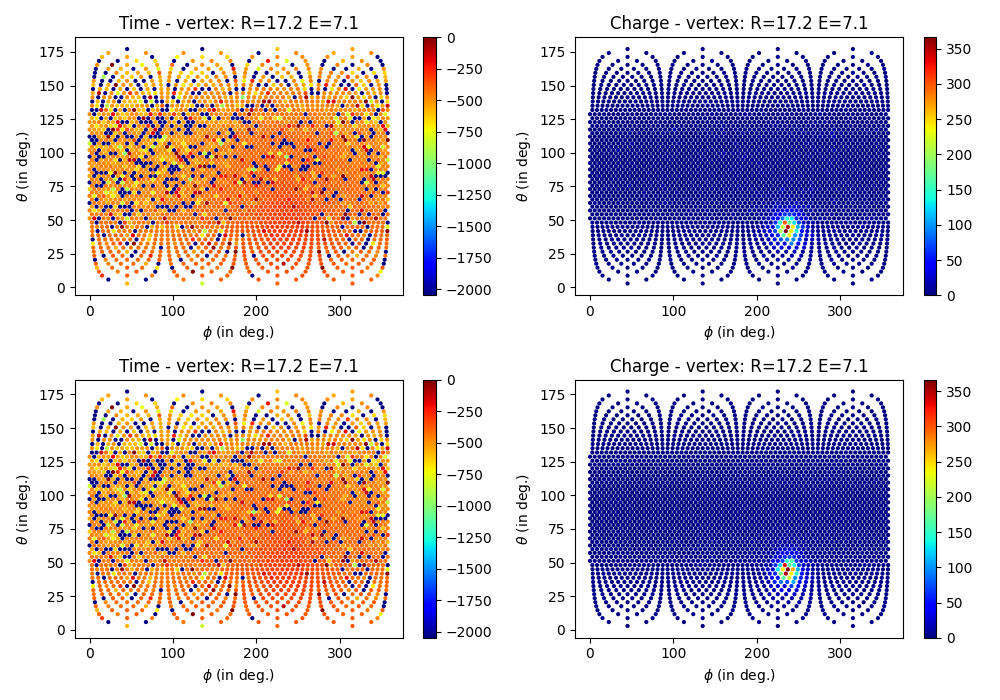
\includegraphics[height=8cm]{images/janne/events/hr_he_400.png}
  \caption{Time channel (on the left) and charge channel (on the right) of a \textbf{radial, high energy event} ($R$ = 17.2 m, $E_{dep}$ = 7.1 MeV), \textbf{Top:} before the ANN perturbation, \textbf{Bottom:} after the ANN perturbation. The ANN have been trained for 400 epochs, just after Phase 2. Time channel in ns and charge channel in $N_{pe}$.}
  \label{fig:janne:hr_he_400}
\end{figure}

\begin{figure}[!ht]
  \centering
  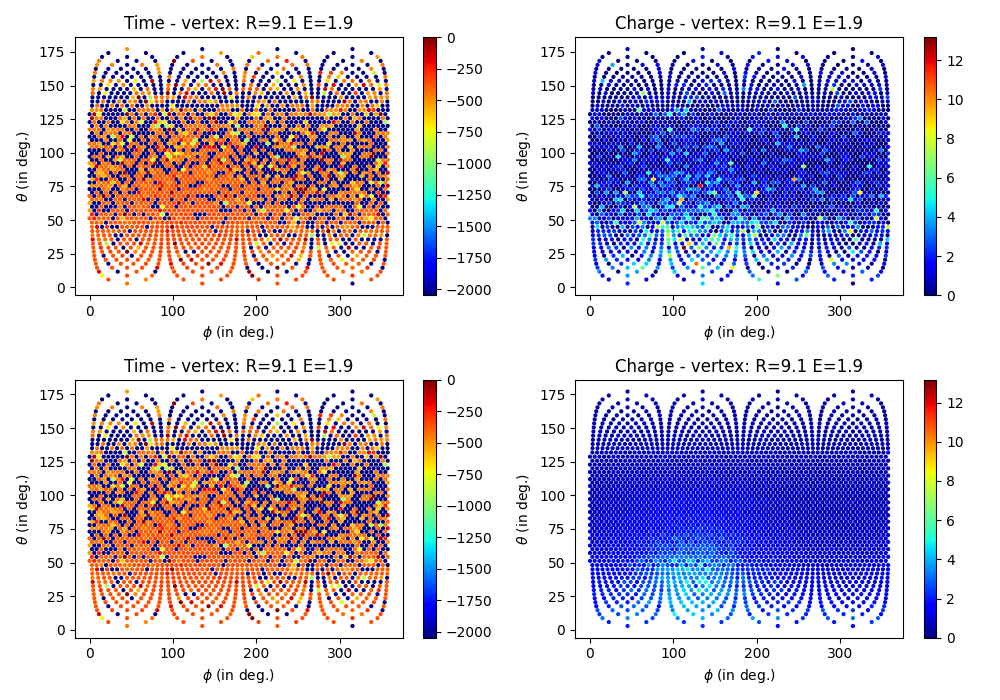
\includegraphics[height=8cm]{images/janne/events/lr_le_400.png}
  \caption{Time channel (on the left) and charge channel (on the right) of a \textbf{central, low energy event} ($R$ = 9.1 m, $E_{dep}$ = 1.9 MeV), \textbf{Top:} before the ANN perturbation, \textbf{Bottom:} after the ANN perturbation. The ANN have been trained for 400 epochs, just after Phase 2. Time channel in ns and charge channel in $N_{pe}$.}
  \label{fig:janne:lr_le_400}
\end{figure}

The same observations that were made after phase 1 still apply after phase 2. The ANN still spreads the charge over multiple pixels for central events, Figure \ref{fig:janne:lr_le_400}, while for radial events it is able to reproduce the small localization of the event.

When looking at the distribution of ratio between the reconstructed energy distribution before and after the application of the ANN, Figure \ref{fig:janne:f_circ_over_f_400}, we observe this time a deficit of events in the high energy bin. This deficit is explained by the comparison between the distribution of relative reconstruction errors, Figure \ref{fig:janne:rec_err_400}, in which we see a small negative bias. This same figure shows a wider loss in resolution when the ANN is present. This is the ANN working to degrade the resolution of the FFNN.

\begin{figure}[!ht]
  \centering
  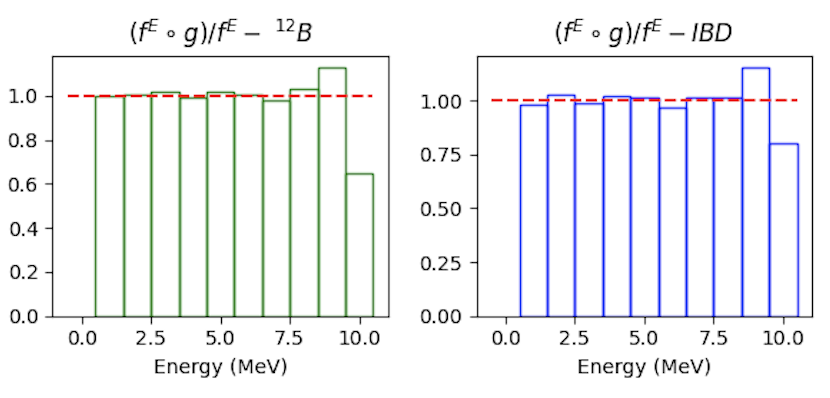
\includegraphics[height=4cm]{images/janne/f_circ_over_f_400.png}
  \caption{Ratio of the reconstructed energy spectra between $({\cal F} \circ {\cal G})$ and ${\cal F}$ at then end of Phase 2 of the training. \textbf{On the left :} For the $^{12}$B dataset. \textbf{On the right :} For the IBD dataset.}
  \label{fig:janne:f_circ_over_f_400}
\end{figure}

\begin{figure}[!ht]
  \centering
  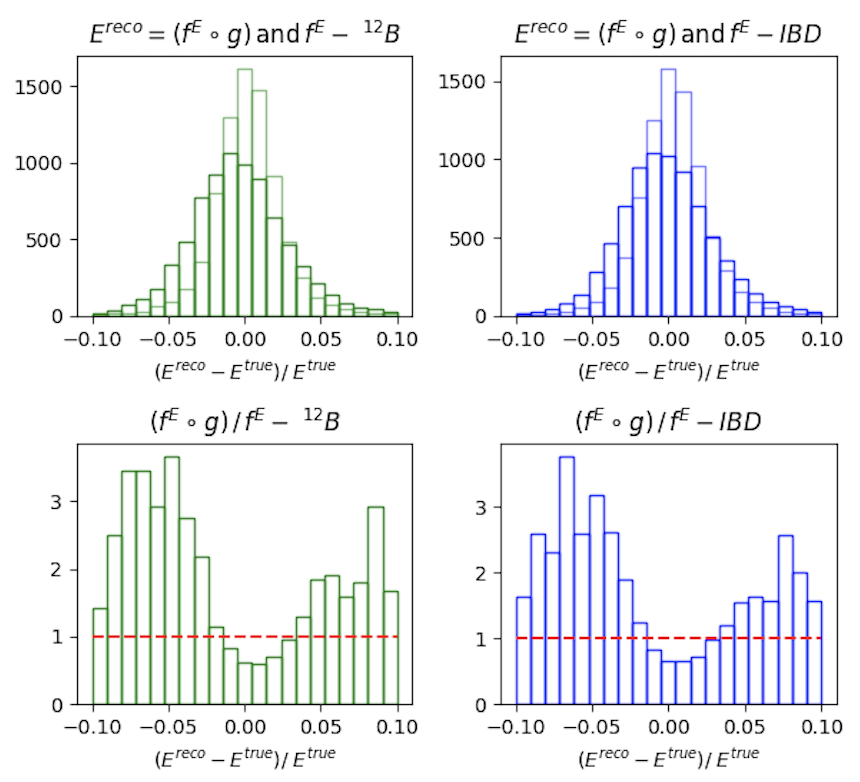
\includegraphics[height=8cm]{images/janne/rec_err_400.png}
  \caption{\textbf{On the top :} Distribution of the relative energy reconstruction error between ${\cal F}$ (light histogram) and $({\cal F} \circ {\cal G})$ (dark histogram) at then end of Phase 2 of the training. \textbf{On the bottom :} Ratio between the light and dark histogram of the top figure.}
  \label{fig:janne:rec_err_400}
\end{figure}

\begin{figure}[!ht]
  \centering
  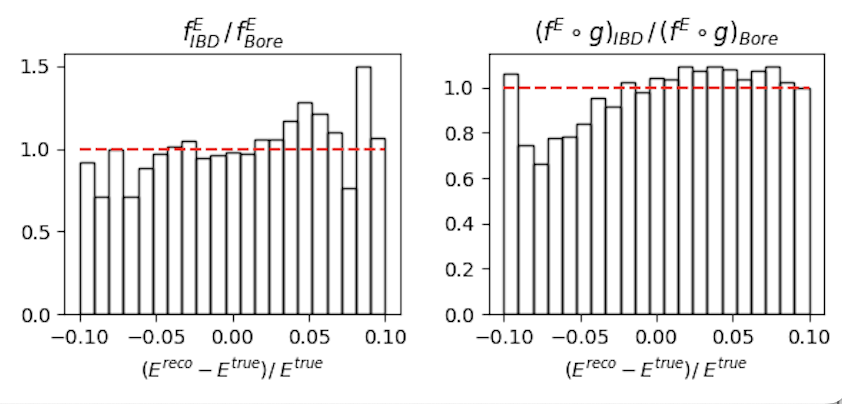
\includegraphics[height=4cm]{images/janne/ann_effect_400.png}
  \caption{Ratio between the relative error on the reconstructed energy between the IBD and the $^{12}$B dataset. \textbf{On the right :} without the ANN. \textbf{On the left :} with the ANN.}
  \label{fig:janne:ann_effect_400}
\end{figure}

Figure \ref{fig:janne:ann_effect_400} shows the ratio between the relative error on the reconstructed energy between the IBD and the $^{12}$B dataset with and without the ANN. We don't see any indicative difference, the ANN even seems to have harmonized the reconstruction error between the two datasets.

In the next section, we will summarize the lessons we gathered while working on this ANN, as well as some perspectives for the future.

\section{Conclusion and prospects}
\label{sec:janne:conclusion}
%\begin{itemize}
%  \item Not enough
%  \item Probably guide the ANN
%\end{itemize}

Reliability and knowledge of our reconstruction algorithms are crucial for the successful conduct of the experiment. The first step to testing and comparing the reconstruction algorithms is to have them publicly available. To this end, I have implemented a BDT for energy reconstruction in JUNO's common software and compared its performance and behavior in detail to the classic likelihood algorithm OMILREC. The strong correlation between their errors indicates that close to no improvement can be made by combining the two algorithms, as they use the same information.

\hfill

Concerning the development of an ANN, we actually developed prototype which was useful to identify several of the difficulties we will have to overcome in the future to produce an ANN fulfilling the aims defined at the beginning of this chapter. First, we determined that learning individual perturbations for each of the 17600 LPMTs (meaning more than 35000 learnable parameters if one decides to perturb $Q$ and $t$) is too much for our available hardware. Then, we determined that particular techniques would be necessary to solve the back propagation problems
described in Section \ref{sec:janne:back_prop} and couple the ANN with any reconstruction algorithm pre-existing in JUNO.

After having opted for a simpler prototype with 3072 learnable parameters, we faced the problem due to their random initialization and adapted by adding a new term to the loss function and splitting the training in 2 phases. Then, we experience the importance of the definition of the loss function, in particular the way to balance two antagonist terms:
one (${\cal L}_{adv}$) which deteriorates the event reconstruction and one that preserves it (${\cal L}_{reg}$). The way to define each of these two terms is not trivial either. Having these notions in mind is essential before trying to develop a tool producing realist perturbation patterns at the individual PMT level.

With this prototype, we manage to produce one of the desired behaviors for such an ANN: we observe ${\cal L}_{adv}$ deteriorating the reconstruction and ${\cal L}_{reg}$ reducing the deterioration. However, at the end of the training, the deterioration is too high compared to the subtle scenarios we want the ANN to produce. A solution against this could be to give a higher weight to ${\cal L}_{reg}$ or to find a more efficient penalty term $P(\epsilon)$.

A smarter definition of ${\cal L}_{adv}$ could also be useful: a definition more explicitly related to our goal (biasing the oscillation analysis) might induce smaller perturbations. This could be a ${\cal L}_{adv}$ favoring a small energy dependent bias between $E_{rec}$ and $E_{dep}$ in IBD events. A smarter ${\cal L}_{adv}$ could also help to produce perturbations that affect the IBD reconstruction more than the reconstruction of $^{12}B$ or calibration events. Although this feature is not mandatory, it would be welcome. It is not achieved by the present version of the ANN.

A possible explanation is the perturbations it produces seem to follow a random pattern across the 3072 pixels. It could be the result of the limited efficiency of the first phase of the training (which tries to recover from the random initialization of these perturbations), or result from the present definition of ${\cal L}_{adv}$ (which can be minimized by random perturbations).

The architecture of the ANN is, for now, very simple; it's a Fully Connected Deep NN with a bottleneck architecture. Previous work in developing ML for reconstruction \cite{qian_vertex_2021} and the algorithms presented in Chapters \ref{sec:jcnn} and \ref{sec:jgnn} show the relevance of convolutions in the reconstruction, and the work of Gavrikov et al.\ \cite{gavrikov_energy_2022} presented at the beginning of this chapter hints at the importance of the time and charge distribution. A more complex and refined architecture can probably be more effective.

Another architecture improvement could come from ResNet architectures \cite{he_deep_2016}. They have already proven that the introduction of residual operations helps the network reach better performance. We can imagine a network where instead of $X' = {\cal G}(X)$ we have $X' = {\cal G}(X) + X$, where the ANN ${\cal G}$ computes only the perturbation instead of a whole new event.

To eventually design an ANN able to perturb several variables for each and every PMT instead of 3072 pixels, we need to find a way to reduce the number of learnable parameters. For instance, the $\delta Q$ perturbation could be a function common to all PMT, depending on learnable parameters controlling its variation against $Q$, $t$  and the position of the PMT. The choice of the function could also be guided by physics informed considerations. To help to learn perturbations affecting IBD events more than others,  the  function could also depend on the initial reconstruction of the  interaction position, since the reconstruction of annihilation gammas depends on it.

Finally, to use this method on every reconstruction algorithm, we must move away from the back-propagation method, for reasons detailed in Section \ref{sec:janne:back_prop}, and use different methods such as Reinforcement Learning.

\end{document}

% \chapter{Discrimination of e+/e- events in JUNO}

\documentclass[../main.tex]{subfiles}
\graphicspath{{\subfix{..}}}
\begin{document}
\chapter{Joint fit between the SPMT and LPMT spectra}
\epigraph{``We demand rigidly defined areas of doubt and uncertainty!''}{Douglas Adams, The Hitchhiker’s Guide to the Galaxy}
\label{sec:joint_fit}
% I)  Introduction globale.
% -------------------------------------
% ... Aborder les points suivants de manière succinte, pour donner une vision d'ensemble...
%
%     + JUNO est une expérience de physique de précision : il sera indispensable de comprendre très précisément les effets de reconstruction. C'est  d'autant  plus un défi que Juno emploie une technologie standard en physique des neutrinos (sphère ou cuve de scintillateur liquide  + PMT) mais l'amène dans une configuration extrême et inédite (très gros volume de scintillation, PMT de 30 pouces, etc...) où comprendre les effets de détection peut s'avérer difficile. Il est possible de rater quelque chose. Pouvoir comparer les données et résultats issus de deux systèmes indépendants, soumis à des problèmes différents, est donc précieux. C'est l'origine du dev de sPMT en plus des LPMT.
%
%     + L'importance cruciale de la maîtrise de la reconstruction : résolution à mieux que 3% et biais très inférieur à 1% sur la connaissance de la non linéarité sous peine d'incapacité à mesurer la NMO.
% Rappeler cet élément majeur : si on se trompe de 1%, on conclut à la mauvaise NMO. Utiliser la figure donnée dans la thèse de Yang pour appuyer ce point.
%
%    + Une source possible de non linéarité difficile à détecter à ce stade est la QNL. (Voir section suivante pour définition complète).
%
%     + La DC répond à cela. Elle interviendra notamment en fournissant des méthodes de calibration permettant de corriger la QNL. Ne pas en dire plus, ref these Yang.
%
%     + Plus generalement : Comparer deux systèmes pour détecter des problèmes sur la calibration ou la reco de l'un des deux. C'est ce que l'on fait dans cette thèse en comparant directement les résultats de la mesure des params d'oscillation.
%
%    + Une difficulté à étudier : la corrélation entre les deux systèmes : pas suffisant de comparer l'écart entre les valeurs centrales aux incertitudes individuelles. Nous proposons dans ce chapitre une exploration préliminaire testant différentes méthodes, en prédisant la sensibilité de ces méthodes à la présence QNL à divers degrés.
%
%   + Plan du chapitre.

JUNO is an experiment of precise measurements, where we try to observe small fluctuation in the energy spectrum and have the ambition to achieve sub-percent precision on the oscillation parameters measurement. It is crucial to understand extremely well the reconstruction and the effect we are dealing with. The challenge reside in the standard technology used in the detector, scintillator observed by PMT, but in a scale never seen before, for scintillator volume as for its PMT. Understanding every effect that goes in the detector can become extremely complicated. Being able to compare the results of the same experiment with two systems is thus precious, this is the origin the dual calorimetry with the LPMT and SPMT system.

The resolution and bias of the reconstruction needs to be extremely well characterized: the target resolution of 3\% \cite{juno_collaboration_juno_2022} is unprecedented as is required to be able to distinguished between Normal Ordering (NO) and Inverse Ordering (IO). The non-linearity uncertainty needs to be contained under 1\% or the risk appear to measure the wrong ordering \cite{han_dual_2021}.

One of the possible non-linearity source, that will be used as a reference source in this chapter, is the charge non-linearity (QNL) that will be detailed in next section. The dual calorimetry will be able to solve this problem, using calibrations method and measurements that will be used to correct it \cite{han_dual_2021}.

More generally, comparing the results of the two system will allow to detect potential issues on the calibration or reconstruction. This is done in this thesis by comparing directly the spectra and oscillation parameters measurements of the two system.

The study of the independents results of the two system can bring some informations \cite{cabrera_multi-calorimetry_2023} but this is missing the important correlation that should be present between the two system: they see the same events, in the same scintillator, their bound to be correlated. We explore in this chapter a preliminary study of the impact of those correlation via multiple methods and the impact of QNL at various degree.

In the next section will discuss the motivations behind this study. In section \ref{sec:joint_fit:approach}, I present the approaches and assumptions in this study. In section \ref{sec:joint_fit:framework} I present the fit framework used and following in section \ref{sec:joint_fit:tech} the technical improvement brought and the difficulties faced during the development. To end this chapter I present the results in \ref{sec:joint_fit:results} and discuss the conclusion and perspectives in \ref{sec:joint_fit:conclusion}.

\section{Motivations}
% II)  Motivations
% --------------------------
%
%   (a) Écart entre les résultats sPMT et LPMT
%       -- Tout écart significatif entre les résultats obtenus avec les deux systèmes signale un problème, et est donc intéressant, quelle que soit l'origine du problème.
%      -- Les deux systèmes ont une sensibilité équivalente à theta_12 et dm2_12. Ce sont donc ces deux paramètres que nous comparerons.
%     -- Pour détecter un écart significatif, on ne peut se contenter de comparer l'écart à la racine de la somme quad des erreurs individuelles. En effet, une grande partie de l'incertitude provient des incertitudes statistiques sur le spectre vrai de l'énergie des antineutrinos. Ce spectre étant le même pour les deux systèmes, les erreurs stats sur spectres reconstruits par les deux systèmes sont très corrélées. Si la reconstruction de l'E avait une résolution et un biais nul dans les deux systèmes, alors l'incertitude statistiques entre les mêmes bins des deux spectres serait 100% corrélée. Dans la réalité, les effets de reconstruction, en partie aléatoires, diminue cette corrélation. Elle reste néanmoins un élément central dans ce travail.
%
%    -- Notre travail dans cette partie de la thèse a été de mettre au point plusieurs tests statistiques pertinents pour détecter un écart entre le système des LPMT et celui des sPMT.
%      + Un premier objectif est de fournir les distributions des tests statistiques dans le cas où il n'existe pas de source de désaccord imprévue entre les deux systèmes. La valeur obtenue dans les données réelles pourra être comparée à ces distributions pour déduire des p-values.
%     + Pour évaluer une sensibilité, nous avons besoin de simuler une différence concrète. Nous choisissons de nous intéresser à un effet plausible, la QNL (voir prochaine sous-section). Nous soulignons cependant que la méthode peut être utile quelle que soit la source d'une différence entre LPMT et sPMT (problème dans la calibration, réglage fin de la simulation insuffisant pour un bon data/MC, etc...)
%
\subsection{Discrepancies between the SPMT and LPMT results}

As discussed in the introduction of this chapter, the SPMT system and the LPMT system will observe the same events. This mean that, after calibration, if the two system show significant differences in their results this is the signal of potential overlook of an effect or problem. Being able to detect such differences is thus crucial as, as discussed above, even the smallest deviation from our model could lead to the impossibility to measure the Mass Ordering (MO) or even worse, wrong our measurement.

The two system are expected to have the same sensitivity to the oscillation parameters $\theta_{12}$ and $\Delta m^2_{21}$ \cite{juno_collaboration_sub-percent_2022}. We will thus rely on the measurement of those two parameters to detect potential discrepancies.

We could just look at the value and compare them to the estimated independent error of the two system, but we believe and will demonstrate in this chapter that the independent study of the two system is missing a lot of informations, and that, by taking into account the statistic and systematic correlations between the two systems, we can produce much more powerful statistical test.

Our work in this chapter is to develop such tools. The first step is, of course, to verify that in the case of no discrepancies, the results are coherent with the independent analysis. This will give us the distribution of those statistical test in absence of discrepancies. When we will have real data, we will be able to compare it to those distribution to obtain a p-value characterizing the absence of those potential discrepancies.

To evaluate the power of our methods, we need to simulate a concrete discrepancy. We decide to study a plausible effect, the Charge Non-Linearity (QNL) that is detailed next section, but the goal of those tools is to be discrepancy agnostic, as those discrepancies could come from a variety of source (calibration issue, insufficient simulation tuning, etc...)

%
%   (b) Explications sur la QNL. (  ~ 1 p)
%
%       -- Rappeler que la réponse en E du détecteur est sujette à plusieurs sources de non linéarité. La principale est la NL dans la scintillation de photons. Une autre source est la QNL.
%
%      -- Définition, origine, etc.
%
%      -- Une façon de modéliser : la formule de Yang sur les Q_LPMT.
%          * Insérer les figures que tu as produites récemment (voir slack le 8 juillet à 17h39 et 17h52) : N_ph/N_ph_qnl vs. Etrue, pour différentes valeurs de gamma_qnl. Cela permet au lecteur de rapidement comprendre l'impact du PB.
%         * Fais le lien entre alpha_qnl et gamma_qnl, pour expliquer que plus tard, on ne testera que avec alpha_qnl, c'est à dire en simulant un effet global sur l'Erec pour générer plus vite.
%         * Dans ces figures, tu t'arrêtes à gamma_qnl = 1% <=> alpha_qnl = 0.3 %, je pense que tu peux aller jusqu'au 5% (regarde ce qui est fait chez Yang et dans la publi multicalo). Aussi bien à 0.5%, qu'à 1% et  qu'à 5%, donne le alpha_QNL correspondant, puis introduis-le dans IBDgen pour produire une spectre oscillé biaisé par la QNL, à comparer dans une figure au spectre sans QNL. Le but est de donner une idée de l'impact sur la NMO.
% En tout cas convaincre qu'il y en a un. Si Steven peut produire un delta-chi2, ce serait super.
%
% Remarques :
%       -- C'est un point important, donc il faut que cela soit auto-contenu au maximum.
%       -- S'inspirer de la publi multicalo, et de la thèse de Yang.
%       -- Citer ces deux sources, mais seulement en complément.
%

\subsection{Charge Non-Linearity (QNL)}
\label{sec:joint_fit:qnl}

The CD energy response is subject of two kind on non-linearity, the first one is the LS response non-linearity where the LS photo-production is not linear with the deposited energy as illustrated in figure \ref{fig:juno:nl:gamma}. The second one is the LPMT response non-linearity where the charge read from the LPMT is not linear in respect to the number of collected Photo-Electron (PE) (see section \ref{sec:juno:calib}).

The LS non-linearity comes from physics sources. Particles interaction in the LS will produce mainly scintillation light as discussed in section \ref{sec:juno:LS} but will also produce some cherenkov light (< 10\% of the collected light). Both mechanisms posses intrinsic non-linearity, for the Cherenkov emission it's dependent on the velocity of charged particle velocity while the scintillation photon-yield follow a so-called Birk's law with a "quenching" effect depending on the energy and type of particle \cite{particle_data_group_review_2020}. This results in a event-wise QNL.

The LPMT response non-linearity can come from sheer saturation when subject to a high rate of photon inducing a gain non-linearity or come from readout effects such as the electronic noise, the overshoot, the integration time window and even the waveform algorithm. All of those effects results in a channel-wise QNL.

Precedent studies \cite{han_dual_2021} suggest a model to emulate this non-linearity response that will be used in this work. We thus define the channel wise non-linearity that would be applied to each LPMT readout
\begin{equation}
  \label{eq:joint_fit:gamma_yang}
  \frac{Q_{rec}}{Q_{true}} = \frac{-\gamma_{qnl}}{9} Q_{true} + \frac{\gamma_{qnl} + 9}{9}
\end{equation}
where $Q_{rec}$ is the reconstructed number of PE by the PMT, $Q_{true}$ is true number of PE that hit the PMT, and $\gamma_{qnl}$ is a factor representing the amplitude of the non-linearity.

We also define an event-wise non-linearity characterized by
\begin{equation}
  \label{eq:joint_fit:alpha_yang}
  \frac{E_{vis}}{E_{true}} = \frac{-\alpha_{qnl}}{9} E_{true} + \frac{\alpha_{qnl} + 9}{9}
\end{equation}
where $E_{vis}$ is the visible energy that can be collected by the detector and $E_{true}$ is the true deposited energy. An example of the effect of such event-wise QNL is presented in figure \ref{fig:joint_fit:spectrums_comp}.

\begin{figure}[ht]
  \centering
  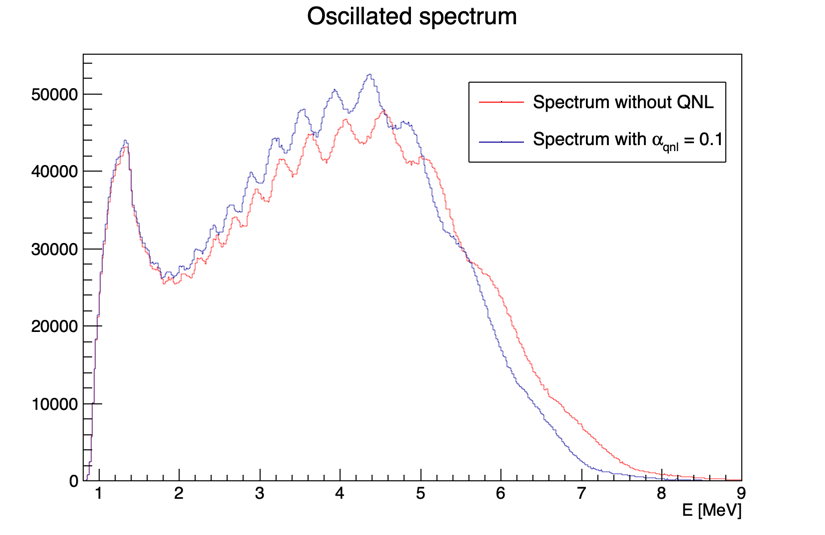
\includegraphics[height=5cm]{images/joint_fit/spectrums.png}
  \caption{Two oscillated spectrums of 1e7 event expected in JUNO. In red the spectrums without supplementary QNL. In blue the same spectrum but where an event-wise QNL $\alpha_{qnl} = 10\%$ is added.}
  \label{fig:joint_fit:spectrums_comp}
\end{figure}


Using 1M from the JUNO official simulation J23.0.1-rc8.dc1 (released the 7th January 2024), we simulated events up to the photon collection in LPMTs and simulated an additional channel-wise QNL by applying the equation \ref{eq:joint_fit:gamma_yang} to the number of collected photons.

\begin{figure}
  \centering
  \begin{subfigure}[t]{0.48\linewidth}
    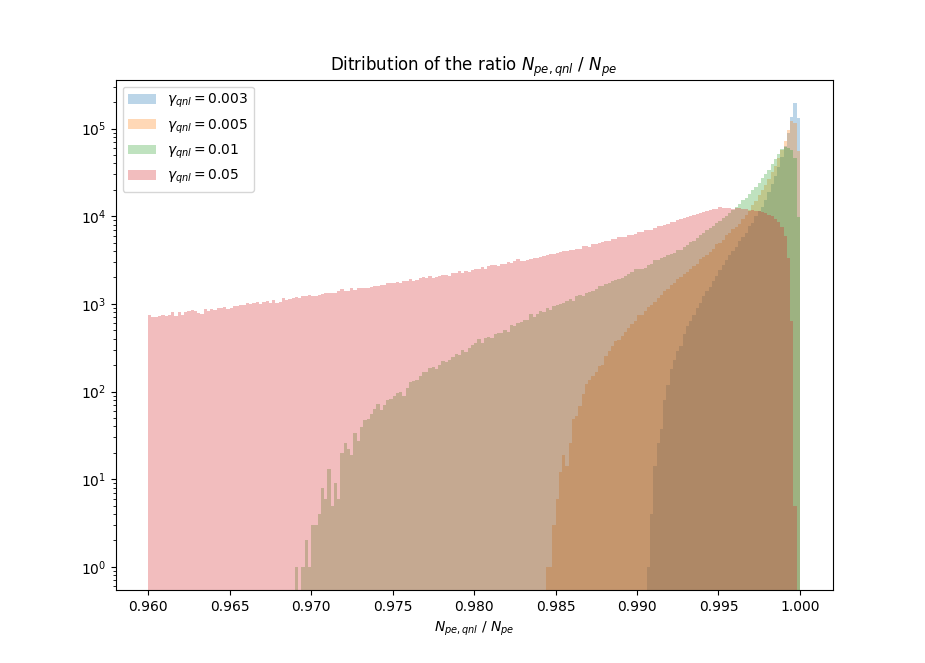
\includegraphics[width=\linewidth]{images/joint_fit/gamma_eff.png}
    \caption{Distribution of ratio of collected nPE after the additional QNL over the number of nPE that would be collected for different $\gamma_{qnl}$. We select event with an interaction radius $R < 4$m to not be affected by the non-uniformity.}
    \label{fig:joint_fit:ratio_distrib}
  \end{subfigure}
  \hfill
  \begin{subfigure}[t]{0.48\linewidth}
    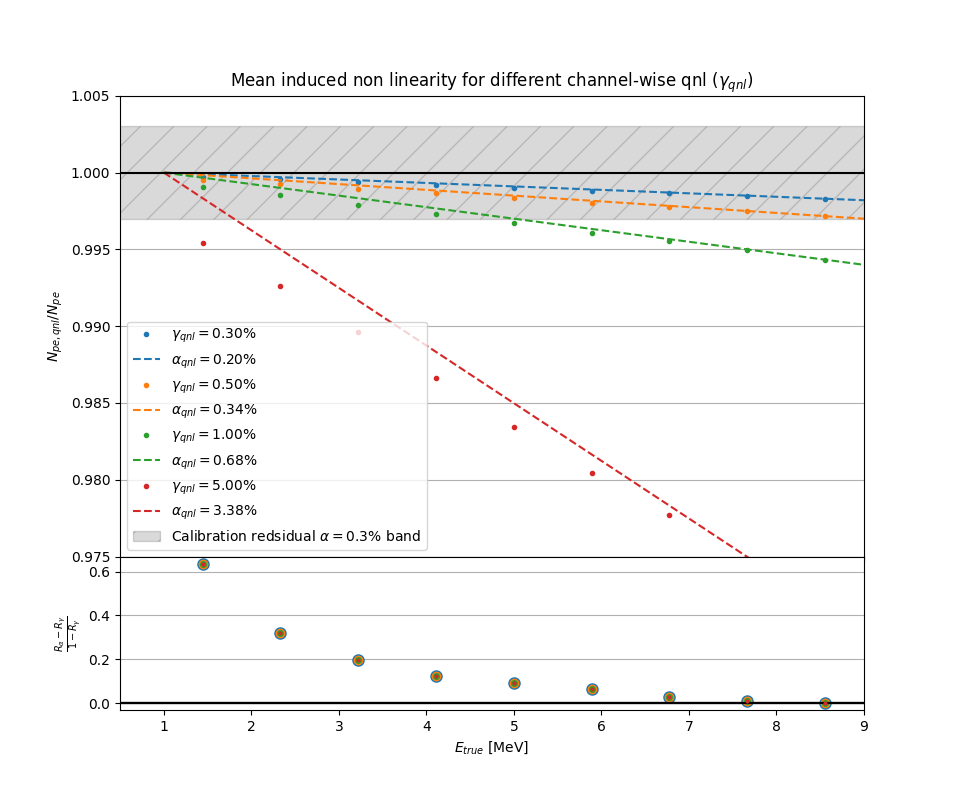
\includegraphics[width=\linewidth]{images/joint_fit/gamma_to_alpha.png}
    \caption{Ratio of collected nPE after the additional QNL over the number of nPE that would be collected at different energies. We select event with an interaction radius $R < 4$m to not be affected by the non-uniformity. The dots represent the mean of the distribution in figure \ref{fig:joint_fit:ratio_distrib} and the dashed line are the equivalent event-wise non-linearity from eq \ref{eq:joint_fit:alpha_yang}. The hatched zone is the residual non-linearity expected after calibration \cite{juno_collaboration_calibration_2021}.}
    \label{fig:joint_fit:gamma_v_alpha}
  \end{subfigure}
  \caption{}
\end{figure}

In figure \ref{fig:joint_fit:ratio_distrib} we show the the distribution of the ratio $\frac{Q_{rec}}{Q_{true}}$ for central events ($R < 4$m) and different value of $\gamma_{qnl}$. In figure \ref{fig:joint_fit:ratio_distrib} we show the mean of this distribution as function of the energy. We show effective $\alpha_{qnl}$ for each value of $\gamma_{qnl}$. We see that using the event-wise QNL is equivalent to the mean behavior of using channel-wise QNL.

When using channel-wise non-linearity, we need to simulate a number of PE per LPMT, the process can be quite tedious if we want a realistic simulation so in this study we are only using event-wize non-linearity to make the process simpler. This event-wise non-linearity will be characterized by $\alpha_{qnl}$.

%  (c) Blinding ?
%  L: Pas expert du sujet (mais alors pas du tout). Je me souviens de la discussion avec steven ou on pourrait ainsi appliquer nos outils avant l'unblidding et ainsi verifier que tout vas bien avant de regarder les resultats ?
%
%
%  (d) Motivations techniques
%
%       -- À compléter à partir de mes notes.
%          Tourne autour de la capacité, utile en général, à réaliser un fit joint.
%  L: En gros dire que c'est pratique de savoir le faire ?

\section{Approach}
\label{sec:joint_fit:approach}

In this section we detail the testing procedure behind each of our tools.

% III) Démarche
% -----------------------
%
%   (a) Simulation d'échantillons toys.
%
%          --- C'est la base de cette étude.
%          --- Dans chaque toy, nous générons un spectre vrai de l'E_nu qui est le point de départ commun de la production des deux spectres reconstruits des LPMT et des sPMt.
%          --- Puis nous ajoutons de façon simplifiée (pas nécessaire d'en dire plus ici, voir la sous - section sur IBDgen) les effets de reco pour avoir dans chaque toy deux spectres.
%          --- Nous étudions plus loin l'effet de la l'exposition sur la sensibilité de la méthode. Donc cet exercice est répété pour plusieurs statistiques (100 jours, 1 an, 2 ans, 6 ans).

\subsection{Data production}

\subsubsection{IBD spectra}

The first step is the generation of data on which we run our tools. In this study we are producing monte-carlo toy. In each toy we generate an $\bar{\nu}_e$ energy spectrum coming from the Taishan, Yangjiang and Dayabay reactor power plant, the reactor used as source for the NMO analysis. The parameters of the reactors come from JUNO official database, shared among all physics analysis, the JUNO common inputs. This is the starting point of the two observed spectrum, the LPMT and SPMT spectrum. On those spectrum, we add the physics effect such as the LS non-linearity etc... (more details in section \ref{sec:joint_fit:framework:ibd-gen}). On top on those effect, we apply the reconstruction resolution of each systems to their respective spectra. We end up with the two LPMT and SPMT spectrum.

We will study the effect of exposure on our methods at different threshold: 100 days, 1 year, 2 year and finally 6 years which is the nominal data taking period for the NMO analysis.

Those spectra are generated for different QNL, $\alpha_{qnl} = 0$, no spectrum distortion, and for $\alpha_{qnl} \in \{0.01, 0.005, 0.003, 0.002, 0.001\}$. As a reminder, the calibration guarantee a residual event-wise non-linearity $\alpha_{qnl} \leq 0.003$ \cite{juno_collaboration_calibration_2021}.

The first test does not require any fitting and we are just comparing the LPMT and SPMT spectra using the expected statistical correlation matrix in the case $\alpha_{qnl} = 0$, for details about the generation of this correlation matrix, refer to section \ref{sec:joint_fit:cov_mat}. This test is the spectrum $\chi^2$ test or $\chi^2_{spe}$ test. In this test we produce a $\chi^2$ representing show the incompatibility between the LPMT and SPMT spectra:
\begin{align}
  \Delta_i &= h_{L,i} - h_{S,i} \\
  U &= A V A^T \\
  \chi^2_{spe} &= \vec{\Delta}^T U^{-1} \vec{\Delta}
\end{align}
Where $h_{L,i}$ and $h_{S,i}$ are the content of the $i$th bin of the LPMT and SPMT bin respectively. $V$ is the covariance matrix of the LPMT + SPMT spectrum. $A$ is a transfers matrix such as:
\begin{equation}
  A_{ij} = \frac{\partial \Delta_i}{\partial h_j} = \frac{\partial(h_{L, i} - h_{S, i})}{\partial h_j}
\end{equation}
Thus $A_{ij} = 1$ if $i = j$ and $A_{ij} = -1$ if $j$ is the SPMT bin corresponding to the $i$ LPMT bin.

This $\chi^2_{spe}$ is minimal when the statistic between the bins of the LPMT and SPMT spectra follow the covariance matrix $V$. By looking at the distribution of this $\chi^2_{spe}$ when $\alpha_{qnl} = 0$ we can produce p-values for the values found when $\alpha_{qnl} \neq 0$.

\subsubsection{Background spectra}

The JUNO common inputs provides only LPMT background spectra. Those background spectra are already smeared by the LPMT resolution and thus needs to be regenrated to be smeared following the SPMT resolution. Luckily the SPMT resolution is greater that the LPMT, alowing us to oversmear the spectrum using
\begin{equation}
  \label{eq:joint_fit:oversmear}
  S(E) = L(E) \star \frac{1}{\sqrt{|\Delta \sigma^2|} \sqrt{2\pi}} e^{-\frac{E^2}{2|\Delta \sigma^2|}}; ~ |\Delta \sigma^2| = \sigma_L^2 - \sigma_S^2
\end{equation}
Where $S(E)$ is the SPMT spectrum, $L(E)$ the LPMT spectrum, $\sigma_L$ and $\sigma_S$ the LPMT and SPMT resolution respectively. This formula is valid under the assumption that the LPMT and SPMT smearing are gaussian and that the LPMT and SPMT have the same bias. Those two assumption are valid in the context of the IBD spectrum production as detailed in section \ref{sec:joint_fit:framework:ibd-gen}.
The demonstration of equation \ref{eq:joint_fit:oversmear} can be found in annex \ref{sec:annex:oversmearing}.


%   (b) Fits séparés
%     --- Fit individuel LPMT puis sPMT dans chaque toy.
%     --- Les N_toys résultats permettent d'établir la corrélation entre les param d'oscillations mesurés par les deux fits quand la génération ne suppose pas d'effets de reco imprévus.
%          => Description du test statistiques

\subsection{Individual fits}

Each of the spectra, LPMT and SPMT, are then fitted individually with and without the presence of QNL over multiples toys. The results allow us to compute the correlation between the oscillations parameters measured by both of the systems when there is no QNL allowing us to compute a $\chi^2$ representing the compatibility between the oscillation parameters measured by the SPMT and by the LPMT. Because the SPMT system is not sensible to thel oscillation parameters $\Delta m^2_{31}$ and $\theta_{13}$, the test is only done on the oscillation parameters $\theta_{12}$ and $\Delta m^2_{21}$. We can thus produce the individual chi square $\chi^2_{ind}$

\begin{align}
  \Delta_\lambda &= \lambda_{L} - \lambda_{S} \\
  \vec{\Delta} &= [ \Delta_{\theta_{12}} ~ \Delta_{\Delta m^2_{21}} ] \\
  U &= A V A^T \\
  \chi^2_{ind} &= \vec{\Delta}^T U^{-1} \vec{\Delta}
\end{align}

where $\lambda_{L}$ and $\lambda_{S}$ are the measured parameters by the LPMT and SPMT systems respectively. The differents $\lambda$ considered are $\theta_{12}$ and $\Delta m^2_{21}$. $V$ here is the $4\times 4$ covariance matrix between the parameters $\theta_{12, L}$, $\Delta m^2_{21, L}$, $\theta_{12, S}$ and  $\Delta m^2_{21, S}$. $A$ is the transfer matrix that allow to compute the covariance matrix de $\vec{\Delta}$ from $V$ following

\begin{equation}
  A_{ij} = \frac{\partial \Delta_i}{\partial j}; ~ i \in \{ \theta_{12}, \Delta m^2_{21} \}; ~ j \in \{ \theta_{12, L}, \Delta m^2_{21, L}, \theta_{12, S}, \Delta m^2_{21, S} \}
\end{equation}

Same as described abose, by comparing the distribution of this $\chi^2_{ind}$ when $\alpha_{qnl} = 0$ and $\alpha_{qnl} \neq 0$ we can compute the power of this test in term of p-values.

%
%  (c) Fit joint
%
%     --- Un fit de chi2, ajustant aux deux spectres 2 pdf distinctes (par la modèle de reconstruction qu'elles supposent).
%
%     --- Les paramètres ajustés par le fit sont :  ...
%
%     --- Les paramètres fixes, ou contraints par un pull term : ...
%
%     --- Les pdf sont distinctes, mais les valeurs des paramètres d'oscillations sont communes aux deux fits.
%
%     --- Pour tenir compte d'un biais dû à un effet de reco imprévu, delta_th et delta_dm ajoutés à th12 et dm2_12 dans la pdf appliquée au spectre LPMT.
%
%     --- Nous avons là par défaut deux spectres de 410 bins, donc un spectre global de 820 bins. Nous effectuons un fit de chi2 : besoin d'une matrice de corrélation. Dans la plupart des fits joints entre spectres (comme lorsque l'on combine plusieurs expériences) la matrice de covariance statistique totale (celle entre les 820 bins dans notre cas) est diagonale car les différents spectres sont indépendants statistiquement. Là, nous avons pour défi de déterminer les corrélations statistiques entre les deux spectres. Expliqué en section xx.
%
%
%    => La statistique de test.

\subsection{Joint fit}

\subsubsection{Standard joint fit}

The final step is to produce a joint fit between the two spectra. In this case we adjust our model, the oscillated spectrum, over two spectrum as the same time. We minimize a $\chi^2_{joint}$ defined over the two spectra, the LPMT and SPMT one
\begin{align}
  \Delta_i &= D_{i} - T_{i} \\
  \chi^2_{joint} &= \vec{\Delta}^T V^{-1} \vec{\Delta}
\end{align}
where $D_{i}$ is the content of the $i$th bin measured, from the data, and $T_{i}$ is the theoretical number of event in this bin. $V$ is the covariance matrix of our spectrum.

$T$ is the fitted function and depend on multiple parameters
\begin{itemize}
  \item The oscillation parameters $\theta_{12}$, $\Delta m^2_{21}$, $\theta_{13}$ and $\Delta m^2_{31}$. Those parameters can be free, have a pull term or be fixed during the fit.
  \item We take into account in the data production the matter effect and parametrize them by the parameter $\rho$ which is the effective rock density between the reactors and the experiment. Same as the oscillation parameters, this parameter can be free, pulled or fixed.
  \item The exposure of the considered data which is just a normalization factor in front of the theoretical spectrum. This parameter is fixed at the start of the fit.
\end{itemize}

In the standard joint fit, the free parameters are $\theta_{12}$, $\Delta m^2_{21}$ and $\Delta m^2_{31}$. $\theta_{13}$ is fixed to the PDG favorite value. Both of the LPMT and SPMT system are sensible to $\theta_{12}$ and $\Delta m^2_{21}$, thus the terms are totally free and the starting value are the PDG nominal. Only the LPMT system is sensible to $\Delta m^2_{31}$, we let it free so we can observe the effect of the deformation on it while the solar parameters $\theta_{12}$, $\Delta m^2_{21}$ are constrained by the SPMT system. To prevent $\Delta m^2_{31}$ to take absurd value, we add a pull term using the PDG nominal value and error
\begin{equation}
  \chi^2_{joint} = \vec{\Delta}^T V^{-1} \vec{\Delta} + \frac{\Delta m^2_{31} - \Delta m^2_{31,PDG}}{\sigma_{31, PDG}}
\end{equation}

$\theta_{13}$ is the parameter on which we are least accurate. It's fixed to nominal value to prevent degeneracy.

The covariance matrix is produced from a correlation matrix $C$
\begin{equation}
  V_{ij} = \sigma_{i} \sigma_{j} C_{ij}
\end{equation}
where $\sigma_{i}$ is the uncertainty on the number of event in the $i$th bin. We consider in this study that the content of each bin follow a Poisson statistic and that thus the uncertainty is $\sigma_i = \sqrt{N_i}$ where $N_i$ is the content of the $i$th bin. The content of each bin can come from two sources the data and the theoretical spectrum $\sigma_i = \sqrt{D_i}$ (Pearson test) and $\sigma_i = \sqrt{T_i}$ (Neyman test). Precedent studies have show that both Pearson and Neyman tests show bias at low statistic, we thus use the Pearson V test where
\begin{equation}
  \chi^2_{joint} = \vec{\Delta}^T V^{-1} \vec{\Delta} + \frac{\Delta m^2_{31} - \Delta m^2_{31,PDG}}{\sigma_{31, PDG}} + \mathrm{ln} | V |
\end{equation}
and the covariance matrix $V$ is computed using the data spectrum for the uncertainty.

The estimation of the covariance is crucial in this study as the strength of this test rely on the systematic and statistical correlations between the LPMT and SPMT spectrum. The generation methods and results of this matrix is detailed in section \ref{sec:joint_fit:cov_mat}.

\subsubsection{Delta joint fit}

Using the same structure we define a second joint fit, the Delta joint fit where, in addition to everything that was discussed above, we add two other parameters $\delta \theta_{12}$ and $\delta \Delta m^2_{21}$ and split the theoretical $T(\theta_{12}, \Delta m^2_{21}, ...)$ spectrum in two
\begin{equation}
\begin{split}
           &T_{LPMT} \equiv T(\theta_{12} + \delta \theta_{12}, \Delta m^2_{21} + \delta \Delta m^2_{21}, ...) \\
           &T_{SPMT} \equiv T(\theta_{12}                     , \Delta m^2_{21}                         , ...)
\end{split}
\end{equation}

If the there is no additional effect between the LPMT and the SPMT spectra, the fit should converge to $\delta \theta_{12} = \delta \Delta m^2_{21} = 0$. By observing the dispersion of those parameter we can define the probability $P(\alpha_{qnl} = 0 | (\delta \theta_{12}, \delta \Delta m^2_{21}))$ and use the median value of $(\delta \theta_{12}, \delta \Delta m^2_{21})$ when $\alpha_{qnl} \neq 0$ to define a sensibility.

The last test we explore in this thesis is to fit the same spectrum with the standard joint fit that we consider as the hypothesis without distortion $H_0$ and the hypothesis where there can be a distortion, the delta joint fit designed as the $H_1$ hypothesis. By looking at the dispersion of $\chi^2_{joint,H_0} - \chi^2_{joint,H_1}$ we can extract a sensibility to potential distortion.

\subsection{Data and theoretical spectrum generation}

To implement the joint fit, we have technically two data spectra and two theoretical spectra. The data in this study are produced using an IBD generator \textit{IBD gen}, see section \ref{sec:joint_fit:framework:ibd-gen}. The theoretical spectrum are produced the same way as data spectrum but with much higher statistics, $10^7$ events to compare with the $\approx 10^5$ events after 6 years. The two spectrum, that we get as a collection of event, are binned in two histograms from 0.8 to 9 MeV of reconstructed energy with bins of 0.02 MeV each resulting in 410 bins per spectrum. An illustration of the theoretical spectrum can be found in figure \ref{fig:joint_fit:delta:theo}. The low number of events in the tail of the spectrum can cause instability due to the low statistic, we thus cut the spectrum at 7.5 MeV / 335 bins for the fit.

\begin{figure}
  \centering
  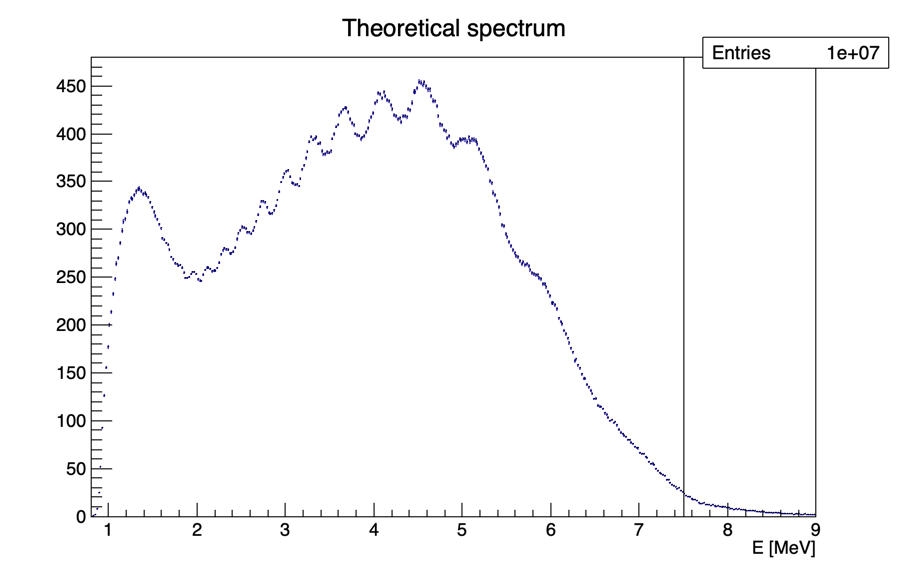
\includegraphics[height=6cm]{images/joint_fit/theoretical_spectrum.png}
  \caption{Theoretical LPMT spectrum at nominal oscillation values binned using 410 from 0.8 to 9 MeV. It is rescaled to correspond to the amount of event expected in 6 years of data taking. The black line represent the 335 bin cut}
  \label{fig:joint_fit:delta:theo}
\end{figure}

%
%   (d) Les suppositions
%
%       --- Nous travaillons en traitant que des erreurs statistiques. Cela se justifie pour un travail exploratoire dans la mesure où une grande partie des effets syst sont totalement corrélés (ceux qui affectent le spectre vrai des neutrinos et des bruits de fond, voir table XX -- systèmatiques du papier Subpercent. )
%
%        --- L'essentiel de nos résultats supposent les effets de détection décorrélés entre LPMT et sPMT. Ils sont par ailleurs introduits de manière simpliste (simple tirage gaussien supposant une résolution gaussienne ne dépendant pas de la position de l'intéraction dans le détecteur --conforme à la publi Subpercent et à la dernière publi NMO). Ce choix se justifie pour un travail exploratoire par la nécessité de produire un grand nombre de toys malgré une puissance de calcul limitée. Un premier raffinement de cette approche tenant compte des corrélations entre les deux reconstructions est présenté en fin de chapitre. Il s'appuie sur la simulation complète du détecteur, et sur notre algo CNN de reco sPMT, le seul disponible à ce jour.
%
%        ---- La QNL est introduite de manière un peu simpliste pour l'instant (appliquée à nouveau juste en fonction de l'énergie de l'IBD). Rappeler que tu as tout de même établi une correspondance (alpha_qnl vs. gamma_qnl) en commençant à faire le boulot qu'il faudrait faire : l'appliquer au niveau des PMT (ce qui tient compte des effets de position de l'intéraction).

\subsection{Limitations}

In this work we are only working considering the statistical errors. We can ignore systematic effects, such as effects that would affect the neutrino spectrum or the background spectrum, as they are entirely correlated between the two systems. The details of those systematic effects can be found in \cite{juno_collaboration_sub-percent_2022}.

Most of our results assume decorrelated detection effects between the SPMT and LPMT system. Their respective reconstruction effect are simulated using simple gaussian drawing on the resolution, independent from their position. This approach was used in previous sensibility and precision studies \cite{juno_collaboration_sub-percent_2022, abusleme_potential_2024}. The potential effect of those reconstruction effects and a first attempt to take them into account are explored in section \ref{sec:joint_fit:cov_mat}.

Even if the goal of this work is to propose deformation agnostic tools, the QNL we use in this study is simplistic as we consider event-wise, position uniform deformation. We show in figure \ref{fig:joint_fit:ratio_distrib} and \ref{fig:joint_fit:gamma_v_alpha} that event-wise QNl is equivalent to the mean behaviour of channel-wise QNL but a more complete study would simulate channel-wise deformation for each event.

\section{Fit software}
\label{sec:joint_fit:framework}

In this section, I describe the ft framework that was used in this study. The software is composed of two part as illustrated in figure \ref{fig:joint_fit:framework}: A standalone part composed of ROOT \cite{brun_root-projectroot_2022} macros, and the Avenue framework.

The Avenue framework is responsible for the spectrum and config reading, transforming the raw collection of event into spectrums, managing the physics effect such as the oscillation, computing and minimizing the $\chi^2$ with the help of the RooFit library. The macros are invoking, if necessary, the Avenue framework and are the entry point for fitting, generating the necessary inputs quantitity such as the spectrums and correlation matrix, analysing the fit results and managing jobs for distributed computing.

\begin{figure}[ht]
  \centering
  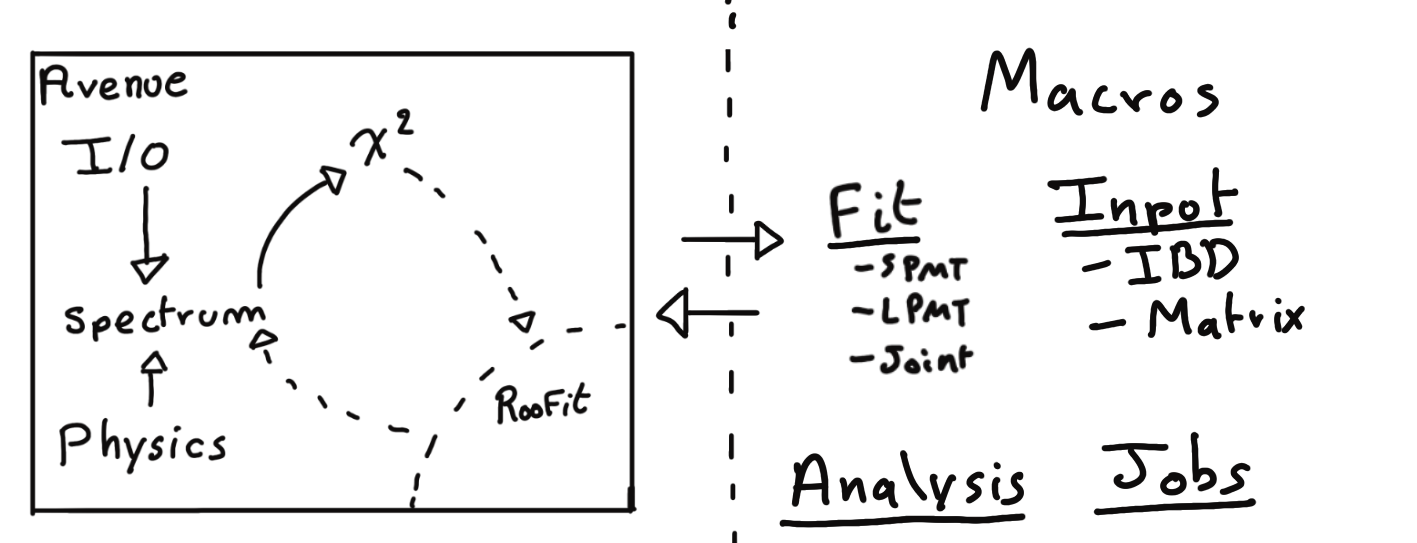
\includegraphics[height=6cm]{images/joint_fit/fit_framework.png}
  \caption{Schematic description of the fit framework}
  \label{fig:joint_fit:framework}
\end{figure}

In this section we will focus on the IBD generator in section \ref{sec:joint_fit:framework:ibd-gen} and the fit macro in itself in section \ref{sec:joint_fit:framework:fit}.
% IV) Le framework de fit.
% ---------------------------------------
%
% ... Description plus ou moins détaillée suivant qu'il a, ou non, déjà été décrit ailleurs...
%
%   (a) Introduction avec rapide overview
%
%
%   (b) La partie standalone : IBD-gen
\subsection{IBD generator}
\label{sec:joint_fit:framework:ibd-gen}

The IBD generator is a standalone generator used to produce oscillated and non oscillated spectrum as seen in the JUNO experiment. It takes as inputs physics parameters and a collection of histograms, values and function provided by JUNO to its analysis groups referred as the JUNO common inputs.

The arguments allow to enable or disable effect such as non-uniformity and non-linearity. It finally take as an argument the number of event to generate $N_{evt}$. Optionally, we generate an effective number of event $N$ by drawing in a Poisson distribution of mean $N_{evt}$.

Then for each event we
\begin{enumerate}
  \item Choose randomly following the reactor power fraction the reactor from which the neutrino come.
  \item Generate a random position in the detector following a uniform distribution in the detector.
  \item Draw a random neutrino energy $E_{\nu}$ from the expected neutrino emission spectrum of every reactor. This spectrum is calculated by:
    \begin{enumerate}
      \item Computing the power spectrum of each isotopes $^{235}$U, $^{238}$U, $^{239}$Pu, $^{241}$Pu using the Huber-Mueller model \cite{huber_determination_2011, mueller_improved_2011}.
      \item Summing the contribution of each isotopes following the respective fission fraction [0.58, 0.07, 0.30, 0.05] as reported in \cite{ma_improved_2013}.
      \item The power of each reactor is then adjusted by their distance from the detector, the detector efficiency and their mean duty cycle (11 of 12 month).
      \item The total spectrum is then finally adjusted by taking into account the correction of the Day Bay bump \cite{daya_bay_collaboration_measurement_2016}, adjustment due to spent nuclear fuel and due to the non-equilibrium.
    \end{enumerate}
  \item \textit{(Optional)} Compute the survival probability due to oscillation at nominal oscillation parameters value. If the neutrino does not survive, the event is rejected and start from step (1).
  \item Compute the emitted positron energy $E_{pos}$ from the mass difference. If the neutrino does not have enough energy reject the event and start from step (1).
  \item Compute the deposited energy $E_{dep}$ by incrementing $E_{pos}$ by 511 keV to account for the positron annihilation. We do not consider cases where some of the energy leak outside of the detector.
  \item Correct the deposited energy with the expected event-wise non-linearity from \cite{juno_collaboration_calibration_2021} to obtain the visible energy $E_{vis}$.
  \item \textit{(Optional)} Add a custom non-linearity as described in section \ref{sec:joint_fit:qnl}. This non linearity is characterized by $\alpha_{qnl}$ to obtain $E_{\alpha}$.
  \item Finally, using the expected resolution of the LPMT and SPMT system provided in the JUNO common inputs, we draw from a gaussian characterized by those resolution the reconstructed energy $E_{rec}$ or $E_{lpmt}$ and $E_{spmt}$ for each system.
\end{enumerate}

The events are stored as n-tuples and are not yet bin at the end of this step.

%
%   (c) Le framework de fit intégré.

\subsection{Fit}
\label{sec:joint_fit:framework:fit}

The fit macro is the core of this fitting procedure. This macro is responsible for loading the fit configuration and setup the Avenue framework. Using Avenue, it will setup the data files, theoretical spectrum, choose the binning, $\chi^2$, etc... It also have the possibility to generate toys on the fly based on the theoretical spectrum. Given this theoretical spectrum we can randomize the bin content either by:
\begin{enumerate}
  \item Drawing the bin content in a Poisson distribution with the bin content as parameter.
  \item Drawing the bin content in a Gaussian distribution with the bin content as mean and variance. The bin content is then rounded to the nearest integer.
  \item Drawing the bin difference following a given covariance matrix using the Choleski decomposition. This matrix is at least the statistical covariance matrix but can also contain systematic uncertainties.
    \begin{align}
      V &= LL^T \\
      \mathbf{R} &\sim \mathcal{N}(0, 1) \\
      \tilde{\mathbf{h}} &= \lceil \mathbf{h} + L\mathbf{R} \rfloor \\
    \end{align}
    where $V$ is covariance matrix used to produce the fluctuations, $\mathbf{R}$ is a draw in a multinomal distribution of mean 0 and variance 1, $\mathbf{h}$ the bin content of the theoretical spectrum and $\tilde{\mathbf{h}}$ the bin content of the generated toy.
\end{enumerate}

The first two methods allow for the fast production of statistics toys while the third allow for the production of statistical and systematical dependent toys. Unfortunately, none of those methods are fitted to produce toy with a QNL different from the theoretical spectrum. The uncertainty on the reconstructed energy $\sigma E_{rec}$ being dependent on $E_{vis}/E_{\alpha}$ makes that we would need to deconvolute the reconstruction effect from the theoretical spectrum. It is much easier to just produce those toys from the IBD generator.

% V) Tes développements techniques.
% -----------------------------------------------------------
%
%   (a) Pour générer les divers toys et pdf dont on a besoin, avec ou sans QNL.
%      --- Bien préciser les deux façons de générer des toys : dans IBDgen, ou dans le fmwk intégré, à partir de la matrice de corr et de Choleski.
%
%    (b)  Pour que le framework intégré soit capable de faire un fit joint.
%
% À ce stade, le lecteur doit comprendre comment tout est fait en pratique, et réaliser la quantité de travail technique que cela a demandé.
\section{Technical challenges and development}
\label{sec:joint_fit:tech}

The fit framework Avenue was already partially developed with multispectrum fitting in mind but a lot technical development was necessary to allow for a joint fit. The first step was to migrate the framework from ROOT5 (last release in March 2018) to ROOT6 (v6.26.06 released in July 2022) to ensure compatibility with the data coming from the JUNO colaboration and benefit of the improvement and corrections that came with ROOT6. This allow us to updgrade the C++ standard from C++11 to C++17. A substantial effort has been done to modernize the code, generalizing the function via templating to help readability and using smart pointer to prevent possible memory leaks.

The Avenue framework had to be adapted, notably on the chi-square calculation and spectrum generation to correctly take into account the correlation between the SPMT and LPMT spectrum. The delta joint fit requiring two more parameters over a spectrum twice as large as before with LPMT takes much more time, around 15h for 6 years exposure, than the single LPMT fit. Thus the framework and the fit macro had to be updated with ditributed calculation in mind. Notably the aggregation of fit results could be done in a single file instead of managing a file per fit. In case of numerous toy, the hard drive access time could lead to long analysis time.

While the IBD generator was already able to generate LPMT and SPMT spectrum, it was not designed for generating correlated spectrum. As detailed in section \ref{sec:joint_fit:framework:ibd-gen}, up to the reconstruction effect, the two spectrum need to share the same generation else the two spectrum would be decorelated and it would be like we would run two different experiment.

\section{Results}
\label{sec:joint_fit:results}
% VI) Résultats
% ----------------------
%
%    (a) Validations techniques.
%
%        i- Les test Asimov sans QNL que nous avions faits, pour valider que le fit joint est OK techniquement (joint vs. Moyenne pondérée des fit individuels) et notamment que la matrice a été mise correctement.
%
%        ii- Tous les autres que je n'ai plus en tête.

\subsection{Validation}

The first step is to confirm that the updated fit framework is able to reproduce existing results and that the joint fit behave as expected, meaning
\begin{itemize}
  \item Without QNL, the individual (\textit{LPMT} and \textit{SPMT}) fit converge to the parameter nominal value and that their errors in the ones reported in existing analysis such as \cite{juno_collaboration_sub-percent_2022}.
  \item The standard joint fit with an independent covariance matrix (\textit{Indep Standard joint}), meaning that the covariance between the LPMT and SPMT spectra is 0, believe to have twice as much information and thus believe to have a grater precision than the the individual fits.
  \item The standard joint (\textit{Standard joint}) fit but with a correlated covariance matrix has errors similiar to the LPMT individual fit as the LPMT drive the precision on $\theta_{13}$ and $\Delta m^2_{31}$ and that the LPMT as SPMT are expected to have the same precision on $\theta_{12}$ and $\Delta m^2_{21}$.
  \item The delta joint (\textit{Delta joint}) fit with covariance matrix have the same resolution as the standard joint fit. The supplementary parameter $\delta \theta_{12}$ and $\delta \Delta m^2_{21}$ should not bring supplementaty precision.
\end{itemize}

The italicized name are the name used in the results reports to identify each fit. We also look into the \textit{Indep Delta joint} which is the fit with the supplementary delta parameters but the covariance between the LPMT and SPMT spectra is 0 and the \textit{Weighted} results where
\begin{equation}
  \frac{1}{\sigma^2_{Weighted}} = \frac{1}{\sigma^2_{LPMT}} \cdot \frac{1}{\sigma^2_{SPMT}}
\end{equation}
We expect the weighted resolution to be similar to the \textit{Indep Standard joint} as, in both of those test, we do not consider the correlation between the SPMT and LPMT results.

\subsubsection{Asimov studies}

We ran the the tests presented above on the updated framework, the results are reported in table \ref{tab:joint_fit:asimov_results}. All those test are ran considering statistics error only, 6 years exposure with all backgrounds, Pearson $\chi^2$ (covariance is estimated using data spectrum) and $\theta_{13}$ fixed to nominal value. For the \textit{SPMT} fit $\Delta m^2_{31}$ is fixed at nominal value as the SPMT system is net expected to be sensitive to this parameter.

\begin{table}[ht]
  \begin{footnotesize}
  \centering
  \begin{tabular}{l | c | c | c | c | c | c }
                                    & $\Delta m^2_{21}$ error  & $\delta \Delta m^2_{21}$ error & $\theta_{12}$ error   & $\delta \theta_{12}$ error  & $\Delta m^2_{31}$ error & $\chi^2$ \\
                                    \hline
  LPMT                                 & 1.29936e-07   &               & 1.33852e-03   &               & 4.39399e-06   & 3.23088e-18 \\
  SPMT                                 & 1.38297e-07   &               & 1.38653e-03   &               &               & 2.87502e-18 \\
  Indep Standard joint                 & 9.48731e-08   &               & 9.86765e-04   &               & 4.39212e-06   & 6.10592e-18 \\
  Standard joint                       & 1.29723e-07   &               & 1.18342e-03   &               & 4.39287e-06   & 3.38055e-18 \\
  Weighted                             & 9.46966e-08   &               & 9.63002e-04   &               &               & \\
  \hline
  Delta joint                            & 1.35780e-07   & 3.43529e-08   & 1.38236e-03   & 1.46865e-04   & 4.39309e-06   & 3.38055e-18 \\
  Indep Delta joint                      & 1.38297e-07   & 1.89391e-07   & 1.38653e-03   & 1.87830e-03   & 4.39241e-06   & 6.10592e-18 \\
  \hline
  \hline
  \multicolumn{7}{c}{Fixed $\Delta m^2_{21}$ and $\Delta m^2_{31}$} \\
  \hline
  Indep Standard joint &               &               & 9.33082e-04   &               &               & 4.82955e-26 \\
  LPMT                 &               &               & 1.27032e-03   &               &               & 2.58849e-26 \\
  SMPT                 &               &               & 1.31070e-03   &               &               & 2.24106e-26 \\
  Weighted             &               &               & 9.12193e-04   &               &               & \\
  \hline
  \hline
  \multicolumn{7}{c}{Fixed $\Delta m^2_{31}$ and$\theta_{12}$} \\
  \hline
  Indep Standard joint          & 8.97117e-08   &               &               &               &               & 6.10617e-18 \\
  SPMT                          & 1.30734e-07   &               &               &               &               & 2.87522e-18 \\
  LPMT                          & 1.23319e-07   &               &               &               &               & 3.23095e-18 \\
  Weighted                      & 8.97066e-08   &               &               &               &               & \\
  \end{tabular}
  \end{footnotesize}
  \caption{Results of the asimov studies of the updated framework. All results are asimov fit, considering 6 years exposure, $\theta_{13}$ is fixed to nominal value, $\chi^2$ is pearson meaning that he error is esitmated using the data spectrum}
  \label{tab:joint_fit:asimov_results}

\end{table}

In every cases presented above, the fit converges to the parameters nominal value thus only the errors are presented.

We observe, as expected, that $\sigma_{Weighted} \approx \sigma_{Indep~Standard~joint}$ with the exception of $\sigma \theta_{12}$. This could from the slight difference in statistic between the SPMT and LPMT spectra. Indeed, due to a larger smearing in energy resolution, event that would be in the spectra range [0.8, 7.5] MeV are smeared outside the spectrum. This deficit is partially compensated by event outside the spectrum coming back in this range but we expect very few event outside the spectrum in comparison to event at the edges of it. Thus the event deficit is not totally compensated. $\theta_{12}$ being mainly driven by the amplitude of the spectrum (see illustration \ref{fig:juno:juno-spectrum-oscillation}), that's why we think this the origin of the difference.

The second observation is that $\sigma_{Standard~joint} \approx \sigma_{LPMT}$. Once the covariance matrix between the LPMT and SPMT is correctly introduced, the fit ``understand'' that it does not have supplementary information and the LPMT system, which have the best precision, dominate the resolution.

Finally for the \textit{Delta} fit, the error on $\delta \theta_{12}$ and $\delta \Delta m^2_{21}$ are of the same order of magnitude than the errors on $\theta_{12}$ and $\Delta m^2_{21}$ in the absence of the covariance matrix. As the LPMT and SPMT spectra are not connected through the covariance matrix, the delta parameters are unconstrained thus the similar errors. Once the covariance matrix is introduced, the delta are much more constrained and present errors an order of magnitude smaller than the error om their respective parameters.

Overall, the asimov studies are satisfactory. The joint fit behave as expected and the errors on the delta parameters are significantly smaller than the error on their respective parameters, indicating great potential if the converge to value different from 0.

\subsubsection{Toy studies}


%   (b) La matrice de covariance
%
%      i- méthode théorique
%         --- explications
%         --- résultats
%      ii- méthode toys
%             Idem
%      iii- la méthode basée sur les données sniper.
%            Idem
%      iv- comparaison
%         --- commentaires et conclusion.
%
%     Préciser ou rappeler ici que
%         --- pour nos tests, nous nous basons sur l'hypo H0 et donc nous générons la matrice sans QNL.
%         --- les corrélations dépendent peu de la forme du spectre ou se sa stat.
\subsection{Covariance matrix}
\label{sec:joint_fit:cov_mat}

%
%   (c) Résultats fit séparés
%
%
%   (d) Résultats fits joints
%
%   (e) Résultats avec corrélations reco_spmt vs. reco_lmpt mieux prises en compte
%

\section{Conclusion and perspectives}
\label{sec:joint_fit:conclusion}
% Vll) Discussions, perspectives

\end{document}


\chapter{Conclusion}

\cleardoublepage

\appendix
\documentclass[../main.tex]{subfiles}
\graphicspath{{\subfix{..}}}
\begin{document}
\chapter{Calculation of optimal $\alpha$ for estimator combination}
\label{sec:annex:jcnn:alpha}

This annex the details of the determination of the optimal $\alpha$ for estimator combination presented in section \ref{sec:jcnn:combination}.

As a reminder, the combine estimator $\hat{\theta}$ of $X$ is defined as
\begin{equation}
  \hat{\theta}(X) = \alpha \theta_N + (1 - \alpha) \theta_C; ~ \alpha \in [0; 1]
\end{equation}
where $\theta_N$ and $\theta_C$ are both estimator of X.

\section{Unbiased estimator}
For the unbiased estimator, it is straight-forward. We search $\alpha$ such as $E[\hat{\theta}] = X$
\begin{align}
  E[\hat{\theta}] &= E[\alpha \theta_N + (1-\alpha) \theta_C] \\
                  &= E[\alpha \theta_N] + E[(1-\alpha) \theta_C] \\
                  &= \alpha E[\theta_N] + (1-\alpha) E[\theta_C] \\
                  &= \alpha (\mu_N + X) + (1-\alpha) (\mu_C + X) \\
                X &= \alpha \mu_N + \mu_C - \alpha \mu_C + X \\
                0 &= \alpha (\mu_N - \mu_C) + \mu_C \\
                \\
                \Rightarrow \alpha &= \frac{\mu_C}{\mu_C - \mu_N}
\end{align}

\section{Optimal variance estimator}

The $\alpha$ for this estimator is a bit more tricky. By expanding the variance we get
\begin{align}
  \mathrm{Var}[\hat{\theta}] &= \mathrm{Var}[\alpha \theta_N + (1-\alpha) \theta_C] \\
                             &= \mathrm{Var}[\alpha \theta_N] + \mathrm{Var}[(1-\alpha) \theta_C] + \mathrm{Cov}[\alpha(1-\alpha) \theta_N \theta_C] \\
                             &= \alpha^2 \sigma_N^2 + (1 - \alpha)^2 \sigma_C^2 + 2\alpha(1-\alpha) \sigma_N \sigma_C \rho_{NC}
\end{align}
where, as a reminder, $\rho_{NC}$ is the correlation factor between $\theta_C$ and $\theta_N$.

Now we try to find the minima of $\mathrm{Var}[\hat{\theta}]$ with respect to $\alpha$. For this we evaluate the derivative
\begin{align}
  \frac{\dd}{\dd \alpha} \mathrm{Var}[\hat{\theta}] &= 2\alpha \sigma_N^2 - 2(1-\alpha) \sigma_C^2 + 2 \sigma_N \sigma_C \rho_{NC} (1- 2\alpha) \\
                                                    &= 2\alpha (\sigma_N^2 + \sigma_C^2 - 2 \sigma_N \sigma_C \rho_{NC}) - 2\sigma_C^2 + 2 \sigma_N \sigma_C \rho_{NC}
\end{align}
then find the minima and maxima of this derivative by evaluating
\begin{align}
  \frac{\dd}{\dd \alpha} \mathrm{Var}[\hat{\theta}] &= 0 \\
  2\alpha (\sigma_N^2 + \sigma_C^2 - 2 \sigma_N \sigma_C \rho_{NC}) - 2\sigma_C^2 + 2 \sigma_N \sigma_C \rho_{NC} & = 0 \\
  2\alpha (\sigma_N^2 + \sigma_C^2 - 2 \sigma_N \sigma_C \rho_{NC}) &= 2\sigma_C^2 - 2 \sigma_N \sigma_C \rho_{NC} \\
  \alpha & = \frac{\sigma_C^2 -  \sigma_N \sigma_C \rho_{NC}}{\sigma_N^2 + \sigma_C^2 - 2 \sigma_N \sigma_C \rho_{NC}} \label{eq:annex:jcnn:sing}
\end{align}
This equation shows only one solution which is a minima. From Eq. \ref{eq:annex:jcnn:sing} arise two singularities:
\begin{itemize}
  \item $\sigma_N = \sigma_C = 0$. This is not a problem because as physicists we never measure with an absolute precision, neither us or our detectors are perfect.
  \item $\sigma_N = \sigma_C$ and $\rho_{CN} = 1$. In this case $\theta_C$ and $\theta_N$ are the same estimator in term of variance thus any value for $\alpha$ yield the same result: an estimator with the same varianve as the original ones.
\end{itemize}

\chapter{Charge spherical harmonics analysis}
\label{sec:annex:jgnn:harms}

When looking at JUNO events we can clearly see some pattern in the charge repartition based on the event radius as illustrated in figure \ref{fig:annex:jgnn:harmonic:events}. When dealing with identifying features and pattern on a spherical plane, the astrophysics community have been using, with success, the spherical harmonic decomposition. The principle is similar to a frequency analysis via Fourier transform. It comes to saying that a function $f(r, \theta, \phi)$, here our charge repartition of the spherical plane constructed by our PMTs, can be expressed
\begin{equation}
  f(r, \theta, \phi) = \sum_{l=0}^{\infty} \sum_{m=-l}^l a^m_l r^l Y^m_l(\theta, \phi)
\end{equation}
where $a^m_l$ are constants complex factor, $Y^m_l(\theta, \phi) = Ne^{im\phi}P^m_l(\cos\theta)$ are the spherical harmonics of degree $l$ and order $m$ and $P^m_l$ their associated Legendre Polynomials. Those harmonics are illustrated in figure \ref{fig:annex:jgnn:harmonic:ill}. By reducing the problem to the unit sphere $r=1$, we get rid of the term $r^l$. The Healpix library \cite{gorski_healpix_2005} offer function to efficiently find the $a^m_l$ factor from a given Healpix map.

\begin{figure}
  \centering
  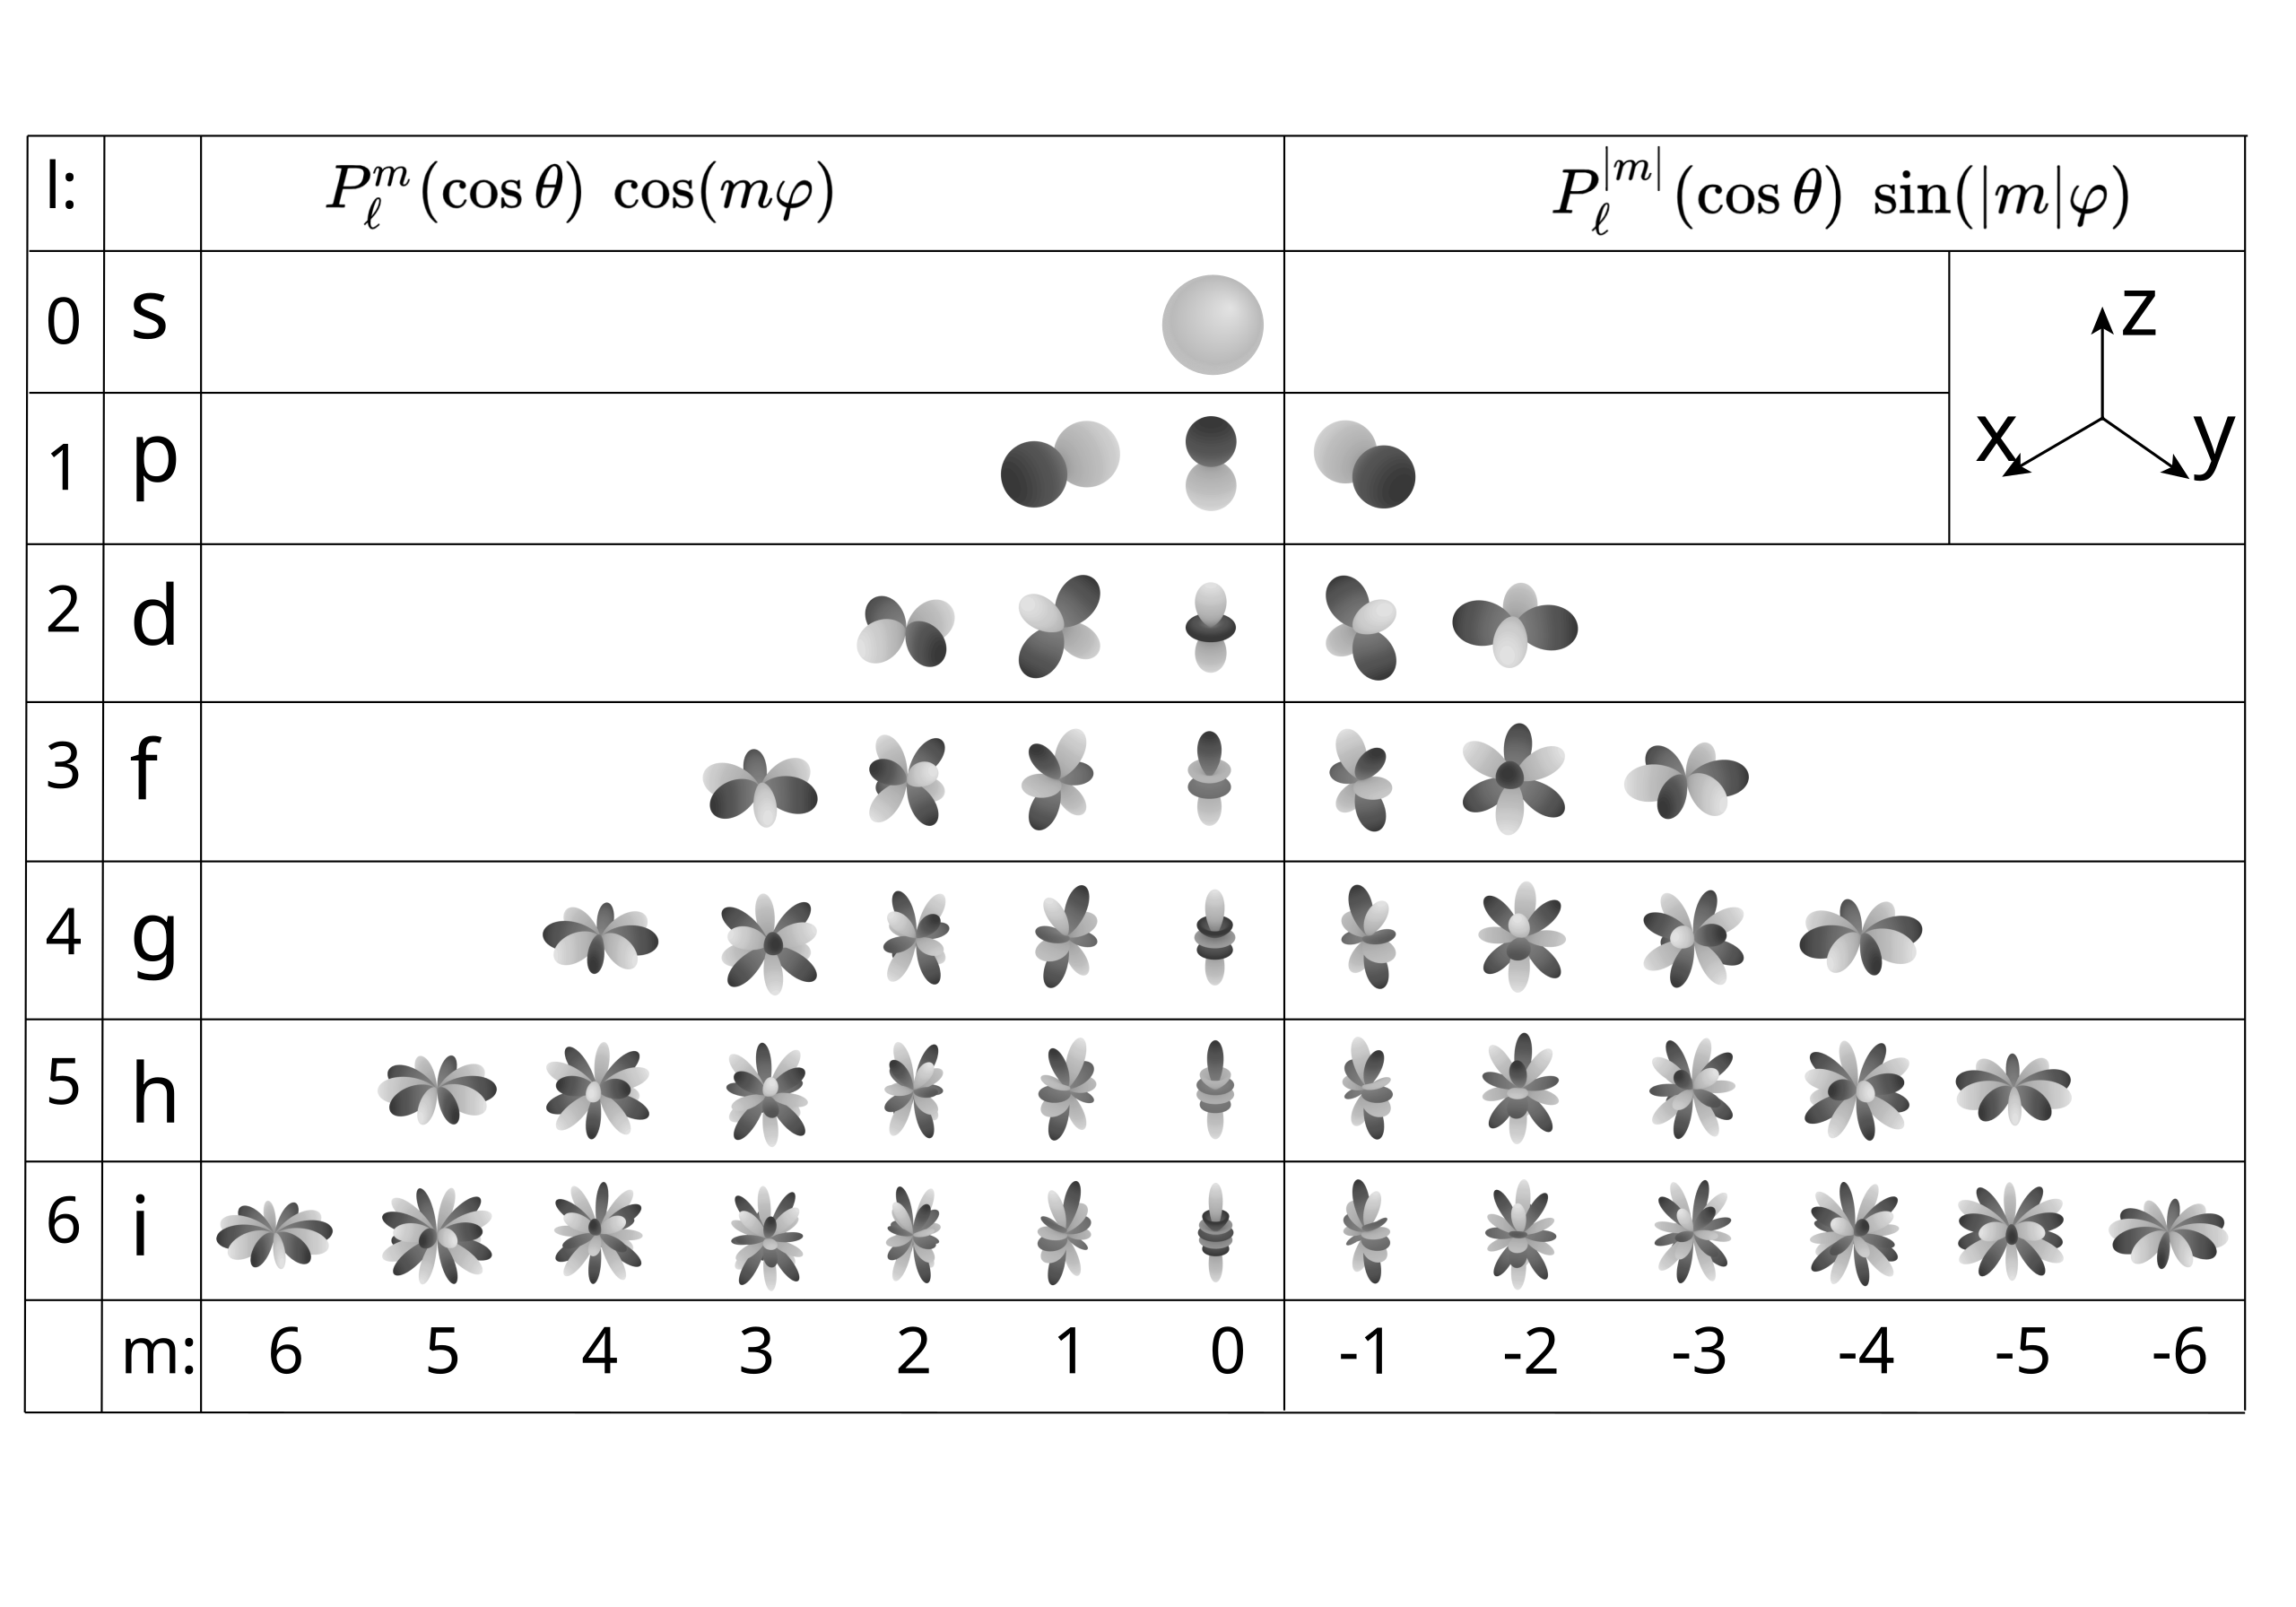
\includegraphics[height=7cm]{images/jgnn/harmonic/harmonics_ill.png}
  \caption{Illustration of the real part of the spherical harmonics}
  \label{fig:annex:jgnn:harmonic:ill}
\end{figure}

For the above decomposition, we will define the \textit{Power} of an harmonic as
\begin{equation}
  S_{ff}(l) = \frac{1}{2l + 1} \sum_{m=-l}^l |a_l^m|^2
\end{equation}
and the \textit{Relative Power} as:
\begin{equation}
  P^h_l = \frac{S_{ff}(l)}{\sum_l S_{ff}(l)}
\end{equation}

For this study we will use 10k positron events with $E_{kin} \in [0; 9]$ MeV uniformly distributed in the CD from the JUNO official simulation version J23.0.1-rc8.dc1 (released the 7th January 2024). All the event are \textit{calib} level, with simulation of the physics, electronics, digitizations and triggers. We first take a sub-set of 1k events and look at the power and relative power distribution depending on the radius and harmonic degree $l$. The results are shown in figure \ref{fig:annex:jgnn:harmonic:radius_dependent}. While don't see any pattern in absolute power, it is pretty clear that there is a correlation between the relative power of $l=0$ and the radius of the event.

\begin{figure}[ht]
  \centering
  \begin{subfigure}[t]{0.48\linewidth}
    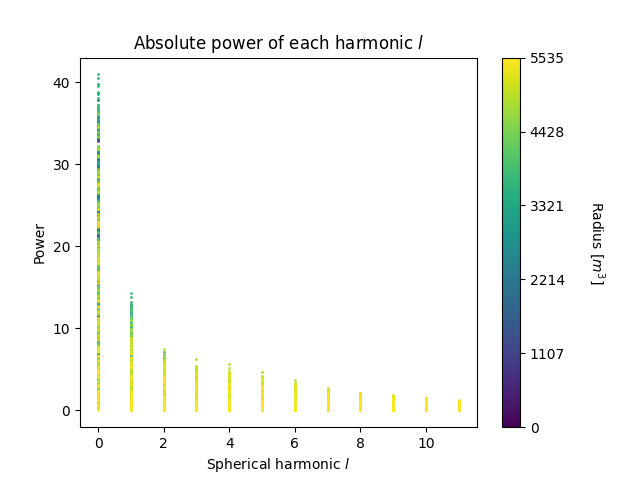
\includegraphics[width=\linewidth]{images/jgnn/harmonic/abs_power_radius_dependency.png}
  \end{subfigure}
  \hfill
  \begin{subfigure}[t]{0.48\linewidth}
    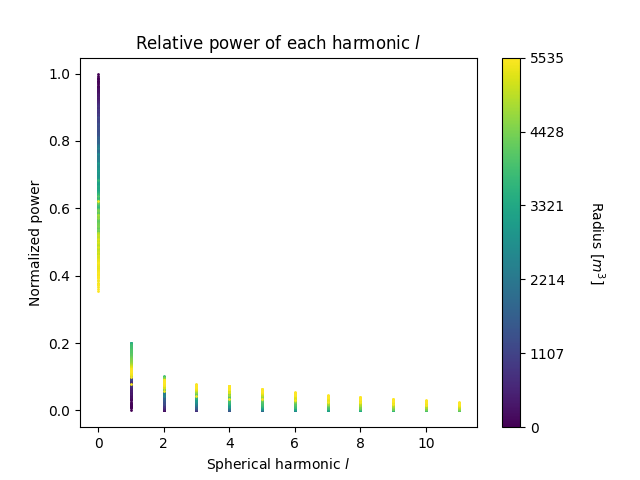
\includegraphics[width=\linewidth]{images/jgnn/harmonic/power_radius_dependency.png}
  \end{subfigure}
  \caption{Scatter plot of the absolute and relative power, respectively on the left and right plot, of each harmonic degree $l$. The color indicate the radius of the event.}
  \label{fig:annex:jgnn:harmonic:radius_dependent}
\end{figure}

When applying the same study but dependent on the energy, no clear correlation appear. The results for the $l=0$ harmonic are presented in the figure \ref{fig:annex:jgnn:harmonic:energy_dependent}. Thus, in this study we will focus on the radial dependency of the relative power of each harmonic.

In figures \ref{fig:annex:jgnn:harmonic:fit1} and \ref{fig:annex:jgnn:harmonic:fit2} are presented the distribution of the relative power of each harmonic for $l \in [0, 11]$. The relation between the radius and the relative power become even more clear, especially for the first harmonics $l \in [0, 4]$. After that for $l > 4$ their relative power is close to 0 for central event, thus loosing power. It also interesting to note the change of behavior in the TR area, clearly visible for $l = 1$ and $l = 2$.

As an erzats of reconstruction algorithm, we fit each of those distribution with a 9th degree polynomial which give us the relation
\begin{equation}
  F(R^3) \longmapsto P^h_l
\end{equation}
We do it this way because some of the distribution have multiple solution for a given relative power, for example $l = 1$, while each radius give only one power. We now \textit{just} need to find
\begin{equation}
  F^{-1}(P^h_l) \longmapsto R^3
\end{equation}
Inverting a 9th degree polynomial is hard, if not impossible. The presence of multiple roots for the same power complexify the task even more. To circumvent this problem, we reconstruct the radius by locating the minima of $(F(R^3) - \hat{P}^h_l)^2$ where $\hat{P}^h_l$ is the measured power fraction.

To distinguish between multiple possible minima, we use as a starting point the radius given by the procedure on $l = 0$ that, by looking at the fit in figure \ref{fig:annex:jgnn:harmonic:fit1}, should only present one minima. For $l > 0$ we also impose bound on the possible reconstructed $R^3$ as $R^3 \in [R^3_0 - 100, R^3_0 + 100]$ where $R^3_0$ is the reconstructed $R^3$ by the harmonic $l=0$.

The minimization algorithm used are the Bent algorithm for $l=0$ and the Bounded algorithm for $l > 0$ provided by the Scipy library \cite{virtanen_scipy_2020}. We then do the mean of the reconstructed radius from the different harmonics. The reconstruction results are shown in figure \ref{fig:annex:jgnn:harmonic:reco}. The performance seems correct but we see heavy fluctuation in the bias. To really be used as a reconstruction algorithm, the method needs to be refined as discussed in the next section.

\begin{figure}[ht]
  \centering
  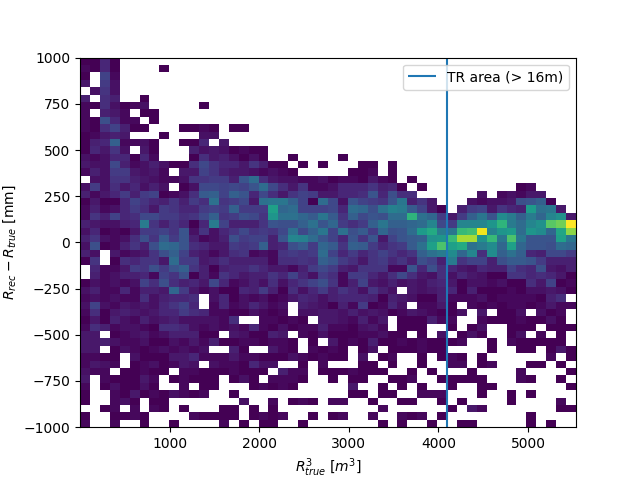
\includegraphics[height=6cm]{images/jgnn/harmonic/Radius_reco.png}
  \caption{Error on the reconstructed radius vs the true radius by the harmonic method}
  \label{fig:annex:jgnn:harmonic:reco}
\end{figure}

\section*{Conclusion}

We have clearly shown in this analysis the relevance the of relative harmonic power for radius reconstruction, and provided an erzats of a reconstruction algorithm. We will not delve further in this thesis but if we wanted to refine this algorithm multiple paths can be explored:
\begin{itemize}
  \item No energy signature in the harmonics: This is surprising that there is no correlation between the energy and the amplitude of the harmonics. We know that the energy is heavily correlated with the total number of photoelectrons collected, it would be unintuitive that we see no relation.
  \item Localization of the event: We shown here the relation between the relative power of the harmonic and the radius but don't get any information about the $\theta$ and $\phi$ spherical coordinates. This information is probably hidden in the individual power of each order $m$ of the degree $l$. This intuition comes from the figure \ref{fig:annex:jgnn:harmonic:ill} where in the higher degree $l$ we see that the order $m$ are oriented. Intuitively, the order should be able to indicate a direction where the signal is more powerful.
  \item Combination of the degree power: Here we combined the radius reconstructed by the different degree via a simple mean but we shown in section \ref{sec:jcnn:combination} and annex \ref{sec:annex:jcnn:alpha} that this is note the optimal way to combine estimator. A more refined algorithm probably exist to take into account the predicting power of each order.
\end{itemize}

\begin{figure}
  \centering
  \begin{subfigure}[t]{0.48\linewidth}
    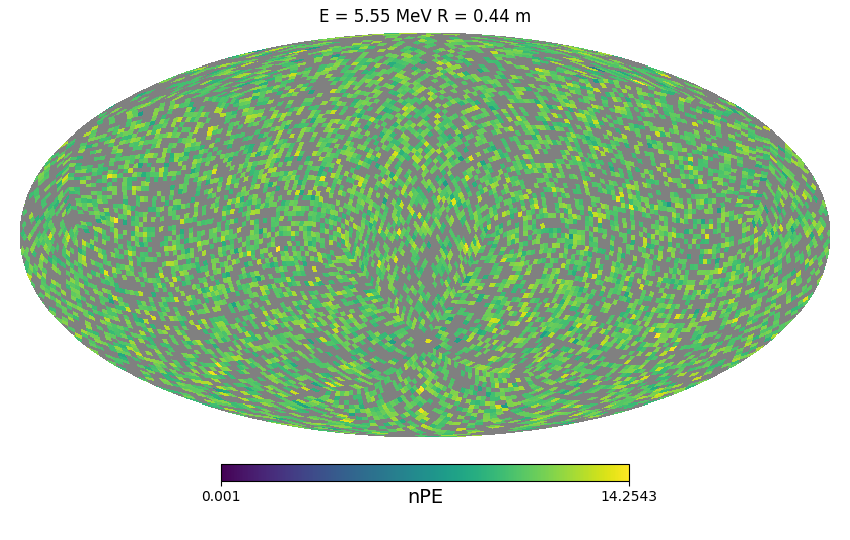
\includegraphics[width=\linewidth]{images/jgnn/harmonic/event_idx_0.png}
    \caption{}
  \end{subfigure}
  \hfill
  \begin{subfigure}[t]{0.48\linewidth}
    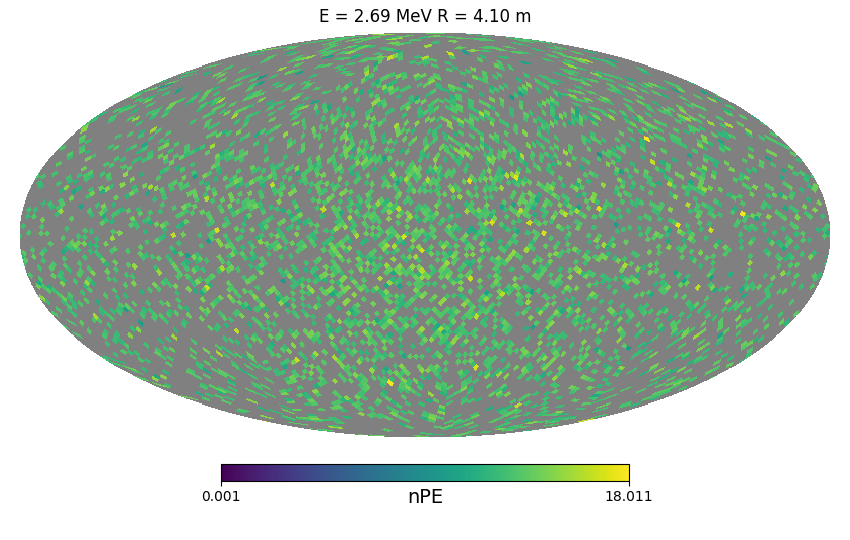
\includegraphics[width=\linewidth]{images/jgnn/harmonic/event_idx_10.png}
    \caption{}
  \end{subfigure}


  \begin{subfigure}[t]{0.48\linewidth}
    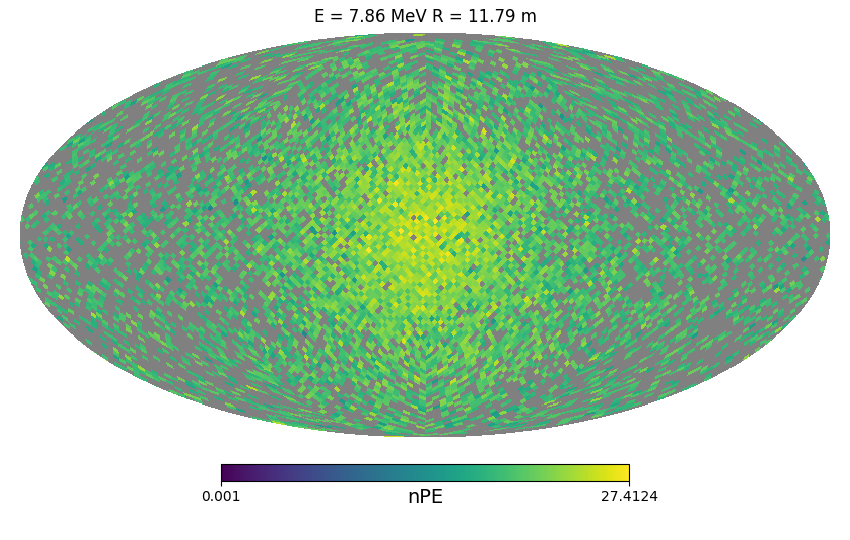
\includegraphics[width=\linewidth]{images/jgnn/harmonic/event_idx_300.png}
    \caption{}
  \end{subfigure}
  \hfill
  \begin{subfigure}[t]{0.48\linewidth}
    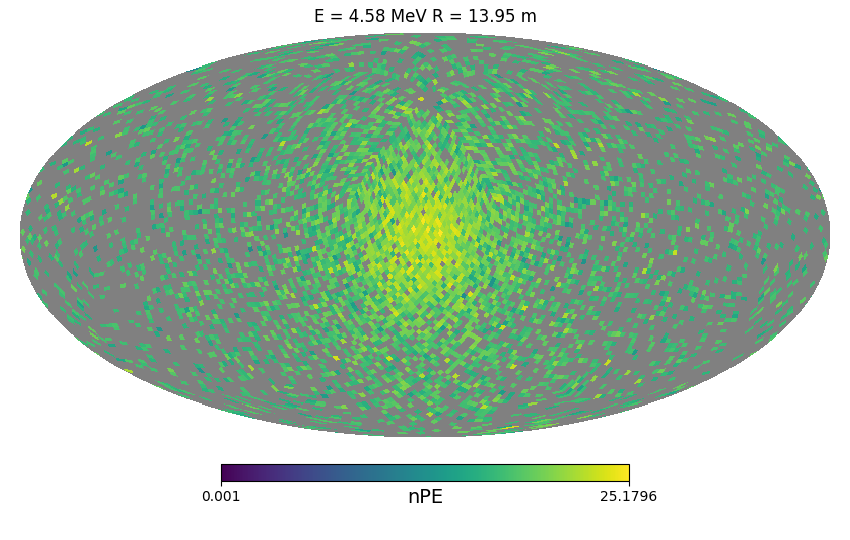
\includegraphics[width=\linewidth]{images/jgnn/harmonic/event_idx_500.png}
    \caption{}
  \end{subfigure}


  \begin{subfigure}[t]{0.48\linewidth}
    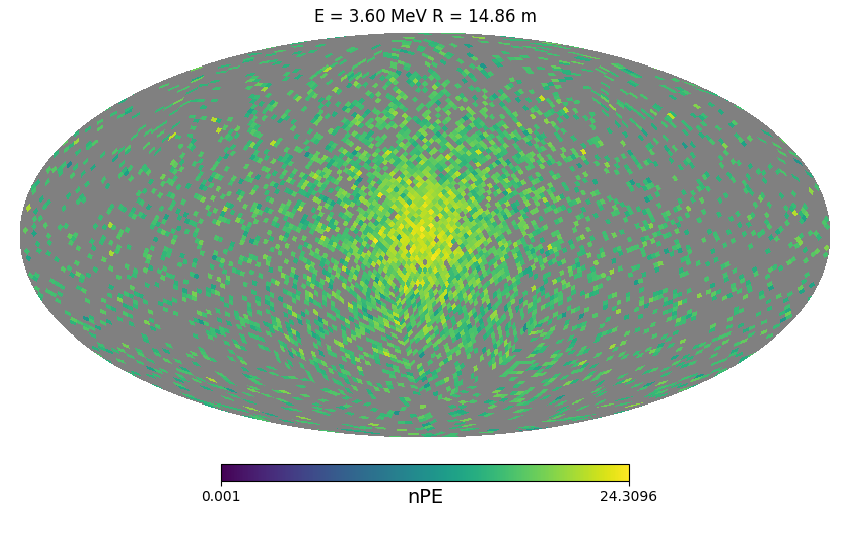
\includegraphics[width=\linewidth]{images/jgnn/harmonic/event_idx_600.png}
    \caption{}
  \end{subfigure}
  \hfill
  \begin{subfigure}[t]{0.48\linewidth}
    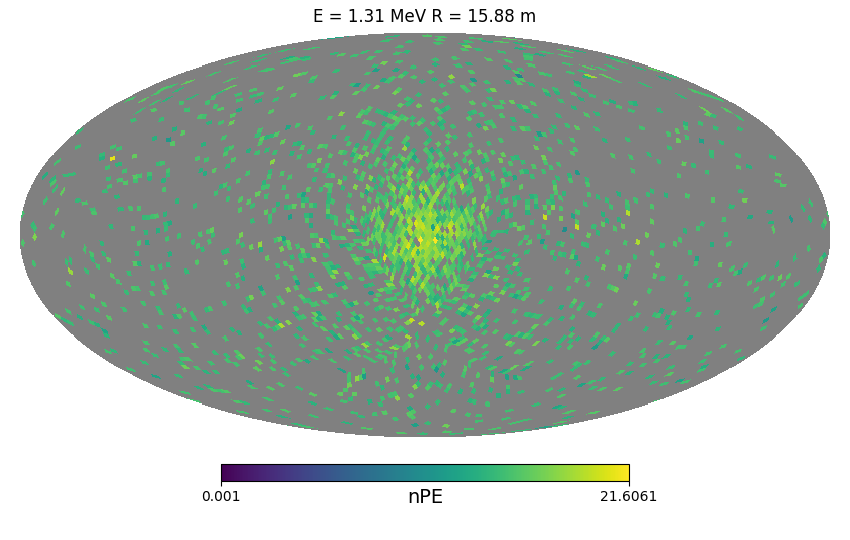
\includegraphics[width=\linewidth]{images/jgnn/harmonic/event_idx_700.png}
    \caption{}
  \end{subfigure}



  \begin{subfigure}[t]{0.48\linewidth}
    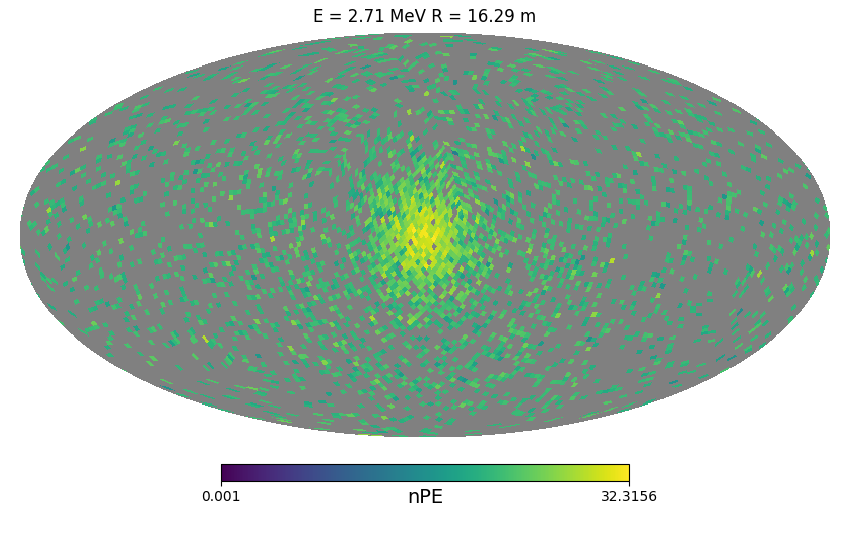
\includegraphics[width=\linewidth]{images/jgnn/harmonic/event_idx_750.png}
    \caption{}
  \end{subfigure}
  \hfill
  \begin{subfigure}[t]{0.48\linewidth}
    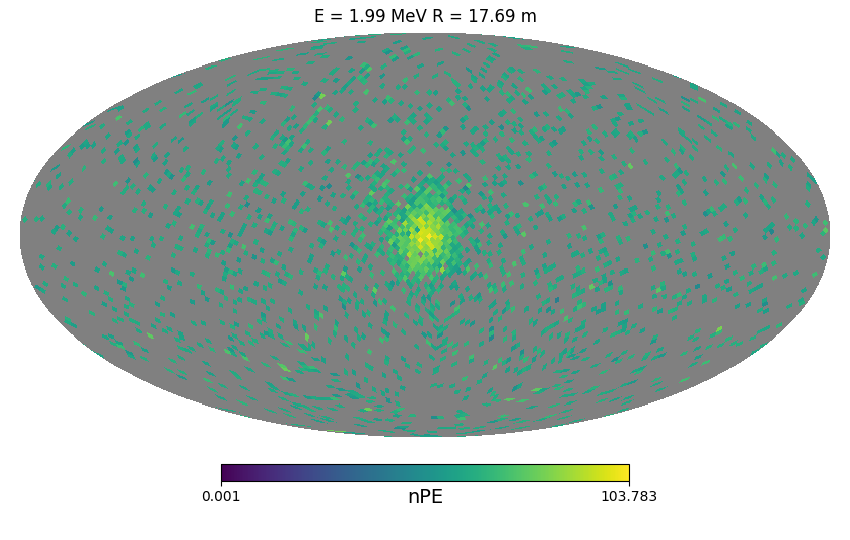
\includegraphics[width=\linewidth]{images/jgnn/harmonic/event_idx_999.png}
    \caption{}
  \end{subfigure}

  \caption{Charge repartition in JUNO as seen by the Healpix segmentation. Those are Healpix map of order 5 (i.e. 12288 pixels). The color represent the summed charge of the PMTs in each pixels. The color scale is logarithmic. The view have been centered to prevent event deformations.}
  \label{fig:annex:jgnn:harmonic:events}
\end{figure}

\begin{figure}[ht]
  \centering
  \begin{subfigure}[t]{0.48\linewidth}
    \includegraphics[width=\linewidth]{images/jgnn/harmonic/power_energy_dependency.png}
  \end{subfigure}
  \hfill
  \begin{subfigure}[t]{0.48\linewidth}
    \includegraphics[width=\linewidth]{images/jgnn/harmonic/rel_power_energy_dependency.png}
  \end{subfigure}
  \caption{Scatter plot of the absolute and relative power, respectively on the left and right plot, of the $l=0$ harmonic. The color indicate the radius of the event.}
  \label{fig:annex:jgnn:harmonic:energy_dependent}
\end{figure}

\begin{figure}[ht]
  \centering
  \includegraphics[width=\linewidth]{images/jgnn/harmonic/power_fit.png}
  \caption{Plot of the distribution of the relative power of each harmonic dependent on $R^3$ (on the left). The Total Reflection (TR) area is represented by the horizontal blue line. The distribution are fitted using a 9th degree polynomial (red curve). The relative power error between the distribution and the fit is represented on the left. \textbf{Part 1}}
  \label{fig:annex:jgnn:harmonic:fit1}
\end{figure}
\begin{figure}[ht]
  \centering
  \includegraphics[width=\linewidth]{images/jgnn/harmonic/power_fit_pt2.png}
  \caption{Plot of the distribution of the relative power of each harmonic dependent on $R^3$ (on the left). The Total Reflection (TR) area is represented by the horizontal blue line. The distribution are fitted using a 9th degree polynomial (red curve). The relative power error between the distribution and the fit is represented on the left. \textbf{Part 2}}
  \label{fig:annex:jgnn:harmonic:fit2}
\end{figure}

\end{document}



\listoftables \addcontentsline{toc}{chapter}{\listtablename}

\cleardoublepage

\listoffigures \addcontentsline{toc}{chapter}{\listfigurename}

\cleardoublepage

\addcontentsline{toc}{chapter}{\abbrevname}
% ============= ABRV ============

\begin{abbreviations}{ll} % Include a list of abbreviations (a table of two columns)

  \textbf{ACU} & \textbf{A}utomatic \textbf{C}alibration \textbf{U}nit \\
  \textbf{BDT} & \ \textbf{B}oosted \textbf{D}ecision \textbf{T}ree \\
  \textbf{CD} & \textbf{C}entral \textbf{D}etector \\
  \textbf{CLS} & \textbf{C}able \textbf{L}oop \textbf{S}ystem \\
  \textbf{CNN} & \textbf{C}onvolutional \textbf{NN} \\
  \textbf{DNN} & \textbf{D}eep \textbf{NN} \\
  \textbf{DN} & \textbf{D}ark \textbf{N}oise \\
  \textbf{FCDNN} & \textbf{F}ully \textbf{C}onnected \textbf{D}eep \textbf{NN} \\
  \textbf{GNN} & \textbf{G}raph \textbf{NN} \\
  \textbf{GT} & \textbf{G}uiding \textbf{T}ube \\
  \textbf{IBD} & \textbf{I}nverse \textbf{B}eta \textbf{D}ecay\\
  \textbf{IO} & \textbf{I}nverse \textbf{O}rdering\\
  \textbf{JUNO} & \textbf{J}iangmen \textbf{U}nderground \textbf{N}eutrino \textbf{O}bservatory \\
  \textbf{LPMT} & \textbf{L}arge \textbf{PMT} \\
  \textbf{LR} & \textbf{L}earning \textbf{R}ate \\
  \textbf{LS} & \textbf{L}iquid \textbf{S}cintillator \\
  \textbf{MC} & \textbf{M}onte \textbf{C}arlo simulation \\
  \textbf{ML} & \textbf{M}achine \textbf{L}earning \\
  \textbf{MSE} & \textbf{M}ean \textbf{S}quared \textbf{E}rror \\
  \textbf{NMO} & \textbf{N}eutrino \textbf{M}ass \textbf{O}rdering\\
  \textbf{NN} & \textbf{N}eural \textbf{N}etwork \\
  \textbf{NO} & \textbf{N}ormal \textbf{O}rdering\\
  \textbf{NPE} & \textbf{N}umber of \textbf{P}hoto \textbf{E}lectron \\
  \textbf{OSIRIS} & \textbf{O}nline \textbf{S}cintillator \textbf{I}nternal \textbf{R}adioactivity \textbf{I}nvestigation \textbf{S}ystem \\
  \textbf{PE} & \textbf{P}hoto \textbf{E}lectron \\
  \textbf{PMT} & \textbf{P}hoto-\textbf{M}ultipliers \textbf{T}ubes \\
  \textbf{PReLU} & \textbf{P}arametrized \textbf{Re}ctified \textbf{L}inear \textbf{U}nit \\
  \textbf{ROV} & \textbf{R}emotely \textbf{O}perated under-LS \textbf{V}ehicle \\
  \textbf{ReLU} & \textbf{Re}ctified \textbf{L}inear \textbf{U}nit \\
  \textbf{ResNet} & \textbf{Res}idual \textbf{Net}work \\
  \textbf{SGD} & \textbf{S}tochastic \textbf{G}radient \textbf{D}escent \\
  \textbf{SPMT} & \textbf{S}mall \textbf{PMT} \\
  \textbf{TAO} & \textbf{T}aishan \textbf{A}ntineutrino \textbf{O}servatory \\
  \textbf{TR Area} & \textbf{T}otal \textbf{R}eflexion \textbf{Area} \\
  \textbf{TTS} & \textbf{T}ime \textbf{T}ransit \textbf{S}pread \\
  \textbf{TT} & \textbf{T}op \textbf{T}racker \\
  \textbf{UWB} & \textbf{U}nder \textbf{W}ater \textbf{B}oxes \\
  \textbf{WCD} & \textbf{W}ater \textbf{C}herenkov \textbf{D}etector \\

\end{abbreviations}

\cleardoublepage

\printbibliography[heading=bibintoc]

\end{document}
